\documentclass{pxcsdoc}
\usepackage{praxfuzz}
\usepackage{parskip}
\usepackage{multicol}
\usepackage{enumerate}
\usepackage{proof}


\newcommand{\true}{\mathrel{\sf true}}
\newcommand{\false}{\mathrel{\sf false}}

\makeindex
\usepackage{trace}

\documentset{Tokeneer ID Station}

\reference{S.P1229.41.2}

\title{Formal Specification}

\synopsis{
This document is the formal specification of the core
Token ID Station (TIS), which forms part of Tokeneer. 
}

\contentsinside

\status{Definitive}

\issuenumber{1.4}

\date{14th August 2008}

\copiedto{%
\begin{minipage}[t]{100mm}%
\vspace{-\abovedisplayskip}%
\begin{multicols}{2}%
\raggedright%
{\bfseries NSA}\\
Randolph Johnson \\[1ex]
{\bfseries SPRE Inc.}\\
\newpage
{\bfseries Praxis High Integrity Systems}\\
Project Team \\[4ex]
~\\
\end{multicols}\end{minipage}
}
\frontsheet{%
Quality
}

\originators{%
Janet Barnes}

\approverA{Approver}{David Cooper}

\confidentiality{}

\begin{document}

\maketitle
%\include{renames}

%=========================================================================

\documentcontrol
Copyright \copyright (2003) United States Government, as represented by the
Director, National Security Agency. All rights reserved.
This material was originally developed by Praxis High Integrity
Systems Ltd. under contract to the National Security Agency.
\section*{Changes History}
\textit{All issues of this document have been type-checked with \fuzz~and have
  given no errors.}
\begin{description}
\item [Issue 0.1] 
(28th March 2003) First draft issued for comments within Praxis.
\item [Issue 0.2]
(5th April 2003) Draft incorporating comments from David Cooper.
\item [Issue 0.3]
(14th April 2003) Draft sent to Randolph Johnson (NSA).
\item [Issue 0.4]
(8th May 2003) Final Draft for formal review.
\item [Issue 1.0]
(9th May 2003) Provisional issue to client following internal review.
\item [Issue 1.1]
(27th June 2003) Definitive issue incorporating client feedback and
correction to faults S.P1229.6.1-5. 
\item [Issue 1.2]
(22nd July 2003) Definitive issue correcting faults 
\begin{itemize}
\item S.P1229.6.6 - Tearing a user token mid-entry should constitute a
failed entry and be logged as such within the statistics.
\item S.P1229.6.7 - Remove the ability to retry fingerprint validation
following a failure.
\item S.P1229.6.19 - Correct typographical error on page 51.
\end{itemize}
\item [Issue 1.3]
(22nd August 2003) Definitive issue correcting faults.
\begin{itemize}
\item S.P1229.6.32 - Improve poor text messages on screen.
\item S.P1229.6.33 - Make initial configuration realistic.
\item S.P1229.6.36 - Screen should show busy message when a user entry
is in progress.
\item S.P1229.6.38 - Operation failures not reported on screen.
\end{itemize}
\item [Issue 1.4]
(14th August 2008) Updated for public release.
\end{description}

\section*{Changes Forecast}

None. This document is now under change control.

\section*{References}
\begin{thebibliography}{99}
\bibitem{Spivey}
The Z Notation: A Reference Manual, J.M Spivey, Prentice Hall, Second Edition,
1992
\bibitem{SRS}
TIS Software Requirements Specification, Version 2.0, S.P1229.41.1.
\bibitem{PP}
TIS Kernel Protection Profile, SPRE Inc, Version 1.0, 5 February 2003.
\bibitem{ST}
TIS Security Target, S.P1229.40.1.
\end{thebibliography}

\section*{Abbreviations}
{\footnotesize\begin{tabular}{ll}
AA           & Attribute Authority \\
ATR          & Answer-to-Reset \\
CA           & Certification Authority \\
I\&A         & Identification and Authentication \\
RSA          & Rivest Shamir Adelman algorithm \\   
SPARK        & SPADE Ada Kernel (analysable Ada subset from Praxis) \\
SRS          & Software Requirements Specification \\
TIS          & Token ID Station \\
\end{tabular}}

%==========================================================================


\tableofcontents


%==========================================================================
\chapter{Introduction}
%==========================================================================
In order to demonstrate that developing highly secure systems to the
level of rigour required by the higher assurance levels of the Common
Criteria is possible, the NSA has asked Praxis High Integrity Systems to
undertake a research project to re-develop part of an existing secure
system (the Tokeneer System) in accordance with their high-integrity
development process. This re-development work will then be used to
show the security community that is is possible to develop secure
systems rigorously in a cost effective manner.

This document is the formal specification, written using the Z
notation. This document specifies the behaviour of the core of the Token
ID Station (TIS) that is being re-developed.
It documents the second step in the Praxis high
integrity systems development approach. The whole process consists of:

\begin{enumerate}
\item
Requirements Analysis (the REVEAL process)
\item
{\bf Formal Specification (using the formal notation Z)}
\item
Design (the INFORMED process)
\item
Implementation in SPARK Ada
\item
Verification (using the SPARK Examiner toolset).
\end{enumerate}

%--------------------------------------------------------------------------
\section{Structure of this Specification}
%--------------------------------------------------------------------------
This specification is a formal model of the TIS core function
presented using the Z notation. 
The specification models TIS as a number of state components and a number of
operations that change the state.  The operations presented in this
specification cover:
\begin{itemize}
\item
user authentication and entry into the enclave;
\item
enrolment of TIS;
\item
administrator logon/logoff;
\item
archiving the log;
\item
updating of configuration data;
\item
shutdown;
\item
overriding the enclave door.
\end{itemize}
This specification specifically does not model user exit from the
enclave; there could also be further administrative operations above
and beyond those presented in this specification but
these are not considered. It is intended that the structure of the
specification should not preclude the addition of further administrative
operations. 

The specification is structured by presenting type constructs useful in the
modelling of TIS in the remainder of this section. 

Section \ref{sec:TIS} introduces the state that defines the TIS.
 
Section \ref{sec:Interfaces} covers accepting data
from the real world and updating the real world. 

Section \ref{sec:Internal} presents a number of partial operations on parts of
the TIS state, these are later used in the construction of the TIS
system operations. 

Section \ref{sec:UserEntry} presents the multi-phase user authentication and
entry operation.

Section \ref{sec:Enclave} describes all the system operations that
take place within the enclave. These are administrative operations.

Section \ref{sec:Start} defines the initial system and the state of TIS at
start-up.

Section \ref{sec:Whole} describes how the whole TIS core
works. Here we pull together the operations described through the remainder
of the specification.

Appendix \ref{chap:readZ} gives a brief introduction to reading Z. 

Appendix \ref{sec:Summary} discusses a number of issues that were raised during the
production of this specification.

Appendix \ref{sec:Pre} gives an informal justification of the
precondition of the whole operation by considering the preconditions
of its constituent parts.

Appendix \ref{sec:SRSTrace} provides a commentary on the tracing of
this document to the SRS \cite{SRS}. It also lists those requirements
from the SRS that do not
trace to the body of this specification. These are categorised by the
reason for exclusion.

Appendix \ref{sec:STTrace} provides a commentary on the tracing of
this document to the Security Target \cite{ST}. 

%--------------------------------------------------------------------------
\section{Trace units}
%--------------------------------------------------------------------------
\label{sec:Traceunit}
Each section of the specification has been tagged with a named {\em
traceunit} which will be used as a reference from later design
documents. All trace units in this document have the prefix ``FS''
identifying them as originating in the Formal Specification.

Most traceunits contain a list of requirements that are relevent to
that part of the specification. These are taken from the SRS
\cite{SRS} and Security Target \cite{ST}. 

For example consider the traceunit on page \pageref{page:firstTraceunit}. Here
the section on tokens is identified by the name {\em FS.Types.Tokens}
and this section is relevant to the satisfaction of a number of
requirements from the Protection Profile \cite{PP} including {\it
FCO\_NRO.2.1}.  
%--------------------------------------------------------------------------
\section{Z basics}
%--------------------------------------------------------------------------
This formal specification is written using the Z formal notation. \cite{Spivey}

%..............................
\subsection{Z comments}
%.............................
The intention is that someone unfamiliar with Z should be able to read this
specification and gain a complete understanding of the functionality
of the TIS system specified within.

We have attempted to make the informal commentary as complete and
unambiuous as possible. We have also separated out the parts of the
commentary that are only relevant for understanding the formal model,
as below:
\begin{Zcomment}
\item
Readers who are not interested in the formal model can skip these
sections of the commentary.
\end{Zcomment}

%...............................
\subsection{Reading Z}
%..............................
Readers of this specification are encouraged to read the Z formal notation. 
Reading the Z in the context of the commentary should disambiguate the
English. 

In Appendix \ref{chap:readZ} we explain the basics of how to read Z. 
These basic ideas should be sufficient to aid reading this
specification. For a more detailed description of the Z notation refer
to \cite{Spivey}.

%....................................
\subsection{Defining Optional Items}
%....................................

In order to be able to define optional items we make the following definitions.

\def\Nil{nil}%
\def\Optional{\mathop{\rm optional}}
\def\The{the~}%

%%pregen \Optional
\begin{zed}
        \Optional X == \{ x : \finset X | \# x \leq 1\}
\\      \Nil[X] == \emptyset[X]
\\      \The[X] == \{~x : X @ \{ x \} \mapsto x \}
\end{zed}

%--------------------------------------------------------------------------
\section{TIS Basic Types}
%--------------------------------------------------------------------------

\begin{traceunit}{FS.Types.Time}
\end{traceunit}

Time and date is some universal clock,
which for our purposes can be modelled as just the naturals.
\begin{zed}
	TIME == \nat
\end{zed}

We define a constant $zeroTime$ used at system initialisation.

\begin{zed}
        zeroTime == 0
\end{zed}

\begin{traceunit}{FS.Types.Presence}
\end{traceunit}

Many entities such as tokens, fingers and floppy disks may be
presented to the system and removed by the user. We monitor the
presence of these entities.
\begin{zed}
	PRESENCE ::= present | absent
\end{zed}

\begin{traceunit}{FS.Types.Clearance}
\end{traceunit}


$CLASS$ is the ordered classifications on document, areas, and people.
\begin{syntax}
	CLASS ::= & unmarked | unclassified | restricted | confidential |
		secret | topsecret
\end{syntax}

There may be other aspects to classification but these are not
modelled here.

\begin{schema}{Clearance}
	class: CLASS
\end{schema}

There is an ordering on the type $Clearance$. The function
$minClearance$  gives the minimum of a
pair of elements of type $Clearance$. This will be the Clearance with
the lowest class. The ordering on class is formally defined within the
design, informally $unmarked$ is the lowest class and $topsecret$ is
the highest class. 

\begin{axdef}
        minClearance : Clearance \cross Clearance \fun Clearance
\end{axdef}

\begin{traceunit}{FS.Types.Privilege}
\end{traceunit}


$PRIVILEGE$ is the role held by the Token user. This will determine
the privileges that the Token user has when interacting with the ID
station.
\begin{syntax}
        PRIVILEGE ::= & userOnly | guard | securityOfficer | auditManager 
\end{syntax}

\begin{traceunit}{FS.Types.User}
\end{traceunit}


A $USER$ is a unique identification of a certificate owner. For the
purpose of this specification it is a given type. 
 
\begin{zed}
	[ USER ]
\end{zed}

\begin{traceunit}{FS.Types.Issuer}
\end{traceunit}


An $ISSUER$ is a unique identification of an issuing body. Issuers are
privileged users with the ability to issue certificates. 
 
\begin{axdef}
ISSUER : \power USER
\end{axdef}

\begin{traceunit}{FS.Types.Fingerprint}
\end{traceunit}


$FINGERPRINT$ will need to include sufficient control information to allow
us to compare with templates and decide a match or not.
\begin{zed}
	[ FINGERPRINT ]
\end{zed}

\begin{traceunit}{FS.Types.FingerprintTemplate}
\end{traceunit}


A $FINGERPRINTTEMPLATE$ contains abstracted information, derived from
a number of sample readings of a fingerprint.

\begin{zed}
	[ FINGERPRINTTEMPLATE ]
\end{zed}

The fingerprint template and will be accompanied by additional information,
such as the threshold level to be applied to any comparisons.
This is not currently modelled.
\begin{schema}{FingerprintTemplate}
	template: FINGERPRINTTEMPLATE
\end{schema}


%--------------------------------------------------------------------------
\section{Keys and Encryption}
%--------------------------------------------------------------------------

\begin{traceunit}{FS.KeyTypes.Keys}
\end{traceunit}

The signing and validation of certificates used in Tokeneer relies on
the use of
asymmetric keys, which comprise two parts, one which is public and
one which is private. 
\begin{zed}
        [ KEYPART ]
\end{zed}

Certificates are signed by an issuer using the private part, and can
be verified by anyone who holds the public part. 

Abstractly, only the public part is visible,
and it is the only part we need to model. In the design we will
introduce the private part too.

Knowing an issuer is equivalent to having a copy of the issuer's
public key part. While possessing an issuer's private key part means 
that you are that issuer.
%--------------------------------------------------------------------------
\section{Certificates, Tokens and Enrolment Data} 
%--------------------------------------------------------------------------
%..........................
\subsection{Certificates}
%.........................

\begin{traceunit}{FS.Types.Certificates}
\end{traceunit}

All certificates consist of data and a signature. A number of
attributes are encoded within the data. Some attributes are common to
all certificates. 

All certificates can be uniquely identified by their issuer and the
serial number supplied by the issuer when the certificate is created.
The only aspect of the certificate ID which is significant at this 
level is the issuer, so we will model the certificate ID as containing
an $ISSUER$ only.
\begin{schema}{CertificateId}
	issuer: ISSUER
\end{schema}

In addition to the unique certificate id all certificates contain a
validity period during which time they are valid. We will model this
validity period as a set of $TIME$s during which they are valid,
which is more general and easier to state. 

Each certificate is signed and can be verified using a key, typically the
public key of an issuer. We model this by associating with each
certificate the key required to validate the certificate. Note that
the key is optional since in the case that the signature or data is
corrupt, no key will validate the certificate.

\begin{schema}{Certificate}
        id: CertificateId
\\	validityPeriod: \power TIME
\\      isValidatedBy: \Optional KEYPART
\end{schema}

Each type of certificate potentially expands on these attributes.

\begin{figure}[htbp]
  \begin{center}
    \leavevmode
    \resizebox{\textwidth}{!}{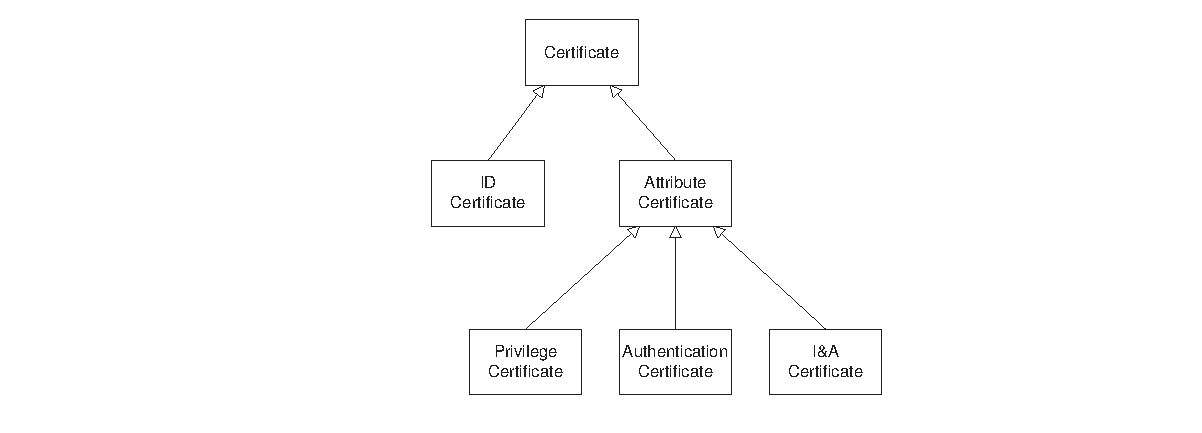
\includegraphics{41_2_certs.eps}}
    \caption{Hierarchy of certificate types}
    \label{fig:certificates}
  \end{center}
\end{figure}

The ID certificate is an X.509 certificate. ID certificates are used
during enrolment as well as being present on tokens.

The subject is the name of the entity being identified by the
certificate and the key is the entity's public key. 

We don't need to know about the key of the Token unless we implement 
the TOKENEER Authentication Protocol or some other secure
comminications protocol between TIS and the Token. Secure
communications with the Token are outside the current scope of this system.

\begin{schema}{IDCert}
	Certificate
\\      subject: USER
\\      subjectPubK: KEYPART
\end{schema}

In general an ID certificate is not validated by the keypart held on
the certificate. 

The ID Certificate of a CA (Certification Authority) is a root
certificate and is signed by itself. The chain of trust has
to start somewhere.

\begin{schema}{CAIdCert}
        IDCert
\where
        isValidatedBy = \{~ subjectPubK ~\} 
\end{schema}


The certificates containing attributes all share some common
attributes. 

All attribute certificates contain the ID of 
the Token and the identification of the ID certificate. Specific types
of attribute certificate build on this common structure.
\begin{schema}{AttCertificate}
        Certificate
\\      baseCertId: CertificateId      
\\      tokenID: TOKENID 
\end{schema}


A privilege certificate additionally contains a role and clearance.
\begin{schema}{PrivCert}
	AttCertificate
\\	role: PRIVILEGE
\\	clearance: Clearance
\end{schema}


An authorisation certificate has the same structure as a privilege certificate.
\begin{schema}{AuthCert}
	AttCertificate
\\	role: PRIVILEGE
\\	clearance: Clearance
\end{schema}

An I\&A (identification and authentication) certificate additionally contains
a fingerprint template. 
\begin{schema}{IandACert}
	AttCertificate
\\	template: FingerprintTemplate
\end{schema}

%..........................
\subsection{Tokens}
%.........................
\label{page:firstTraceunit}
\begin{traceunit}{FS.Types.Tokens}
\traceto{FCO\_NRO.2.1}
\traceto{FCO\_NRO.2.2}
\traceto{FCO\_NRO.2.3}
\traceto{FDP\_DAU.2.1}
\traceto{FDP\_DAU.2.2}
\traceto{FIA\_UAU.3.1}
\traceto{FAI\_UAU.3.2}
\end{traceunit}
\begin{Zcomment}
\item 
Refer to Section \ref{sec:Traceunit} for explanation of the
above tracing block.
\end{Zcomment}
Each Token has a unique ID, ensured unique by the smartcard supplier.
\begin{zed}
	[ TOKENID ]
\end{zed}

A $Token$ contains a number of certificates. The
authorisation certificate is optional while the others must be present.
\begin{schema}{Token}
	tokenID: TOKENID

\also	idCert: IDCert
\\	privCert: PrivCert
\\	iandACert: IandACert
\\	authCert: \Optional AuthCert
\end{schema}


A $Token$ is valid if all of the certificates on it are well-formed,
each certificate correctly cross-references to the ID Certificate,
and each certificate correctly cross-references to the $Token$ ID.

A token need not contain a valid Authorisation certificate to be considered valid.

\begin{schema}{ValidToken}
	Token
\where
	privCert.baseCertId = idCert.id
\\	iandACert.baseCertId = idCert.id

\also	privCert.tokenID = tokenID
\\	iandACert.tokenID = tokenID
\end{schema}

If the Authorisation certificate is present it will only be used if it
is valid, in that it correctly cross-references to the $Token$ ID and
the ID Certificate.

\begin{schema}{TokenWithValidAuth}
	Token
\where
        authCert \neq \Nil 
\\      \t1    \land  (\The authCert).tokenID = tokenID
\\	\t1    \land  (\The authCert).baseCertId = idCert.id
\end{schema}

A $Token$ is current if all of the Certificates are current,
or if only the Auth Cert is non-current.
Currency needs a time, which is included in the schema,
and will need to be tied to the relevent time when this schema is used.

\begin{schema}{CurrentToken}
	ValidToken
\\	now: TIME
\where
	now \in idCert.validityPeriod
\\ \t1		{} \cap privCert.validityPeriod
\\ \t1		{} \cap iandACert.validityPeriod
\end{schema}

%............................
\subsection{Enrolment Data}
%............................

\begin{traceunit}{FS.Types.Enrolment}
\traceto{FMT\_MSA.2.1}
\traceto{FMT\_MTD.3.1}
\end{traceunit}
Enrolment data is the information the ID station needs in order to
know how to authenticate tokens presented to it, and to produce its
own authentication certificates such that they can be authenticated by
workstations in the enclave.

Enrolment data consists of a number of ID certificates: 
\begin{itemize}
\item
this ID Station's ID Certificate, which will be signed by a CA.
\item
A number of other Issuers' ID Certificates. These will belong to 
        \begin{itemize}
        \item
        CAs, who authenticate AAs (Attribute Authorities) and ID Stations. These will be self signed.
        \item
        AAs, who authenticate privilege and I\&A certificates. 
        \end{itemize}
\end{itemize}

The ID Station's certificate is just one of the issuer certificates,
although we will want to be able to identify it as belonging to this
ID station. 

\begin{schema}{Enrol}
        idStationCert : IDCert
\\      issuerCerts : \power IDCert
\where
        idStationCert \in issuerCerts
\end{schema}

For the Enrolment data to be considered valid each certificate must be
signed correctly and the Issuer's certificate must be present for it
to be possible to check that the signatures are correct.
Note that CA ID
certificates are self signed but AA and IDStation certificates are
signed by an CA.

\begin{schema}{ValidEnrol}
        Enrol
\where
        issuerCerts \cap \{ CAIdCert \} \neq \emptyset
\also
\\      \forall cert : issuerCerts @ 
\\      \t1     cert.isValidatedBy \neq \Nil 
\\      \t1     \land (\exists issuerCert : issuerCerts @ 
        issuerCert \in CAIdCert 
\\      \t2     \land \The cert.isValidatedBy = issuerCert.subjectPubK
\\      \t2     \land cert.id.issuer = issuerCert.subject )   
\end{schema}
\begin{Zcomment}
\item
There must be an ID certificate for at least one CA.
\item
For each certificate the enrolment data must include the ID
certificate for the issuer of the certificate, the certificate must be
validated by the issuer's key and the issuer of the
certificate must be a CA.
\end{Zcomment}

%--------------------------------------------------------------------------
\section{World outside the ID Station}
%--------------------------------------------------------------------------
We choose to model the real world (or at least the real peripherals)
as being outside the ID Station.
When the user inserts a token, they are providing input to the ID Station.
It is up to the ID Station to then respond by reading the real world
input into its own, internal representation. The ID Station receives stimulus
from the real world and itself changes the real world. All real world
entities are modelled as components of the $RealWorld$.

We will distingush between real world entities that we use
 (eg. $finger$), we control (eg. $alarm$) 
 and we may change (eg. $userToken$ or $floppy$).


%..............................
\subsection{Real World types}
%..............................

\begin{traceunit}{FS.Types.RealWorld}
\end{traceunit}


There are several types associated with the real world. The door,
latch and alarm all have two possible states.
\begin{zed}
	DOOR ::= open | closed
\also
	LATCH ::= unlocked | locked
\also
	ALARM ::= silent | alarming
\end{zed}

Display messages are the short messages presented to the user on the
small display outside the enclave.
\begin{zed}
	DISPLAYMESSAGE ::= blank | welcome | insertFinger | openDoor |
                        wait | 
\\      \t3  removeToken | tokenUpdateFailed | doorUnlocked
\end{zed}

The messages that appear on the display are presented in table \ref{table:display}.

\begin{table}[h]
\begin{tabular}{|l|l|l|}
                & \multicolumn{2}{c|}{\bf Displayed text} \\ \cline{2-3}
{\bf Message}   & {\bf Top line}                & {\bf Bottom line}     \\
\hline
$blank$         & {\tt SYSTEM NOT OPERATIONAL}  & \\
$welcome$       & {\tt WELCOME TO TIS}          & {\tt ENTER TOKEN}  \\
$insertFinger$  & {\tt AUTHENTICATING USER}     & {\tt INSERT FINGER} \\ 
$wait$          & {\tt AUTHENTICATING USER}     & {\tt PLEASE WAIT} \\
$openDoor$      & {\tt }                        & {\tt REMOVE TOKEN AND ENTER} \\
$removeToken$   & {\tt ENTRY DENIED}            & {\tt REMOVE TOKEN} \\
$tokenUpdateFailed$ &                   & {\tt TOKEN UPDATE FAILED }
\\
$doorUnlocked$  &                       & {\tt ENTER ENCLAVE} \\
\hline
\end{tabular}
\caption{Display Messages}
\label{table:display}
\end{table}

Because it is possible to be trying to read a token that is not inserted,
or a fingerprint when no finger is inserted,
or an invalid token or fingerprint, 
we introduce free types to capture the absence or poor quality of these.

The values $badFP$ and $badT$ represent all possible error codes that
occur when trying to capture this data. The system will behave the
same way in all failure cases with only the audit log capturing the
different error codes that actually occur.
\begin{zed}
	FINGERPRINTTRY ::= noFP | badFP | goodFP \ldata FINGERPRINT \rdata
\also
	TOKENTRY ::= noT | badT | goodT \ldata Token \rdata
\end{zed}

When modelling data supplied on a floppy disk we model the posibility
of the disk not being present, being empty or being corrupt as well as
containing valid data.
We make the assumption that each floppy disk will only contain one
data file, either enrolment data, configuration data or audit data.

\begin{zed}
       FLOPPY ::=  noFloppy | emptyFloppy | badFloppy | 
       enrolmentFile \ldata ValidEnrol \rdata |
\\ \t3    auditFile \ldata \finset Audit \rdata |
          configFile \ldata Config \rdata
\end{zed}

Inputs may be supplied by an administrator at the keyboard. We model
input values representing no data, invalid data or a valid request to
perform an adminstrator operation.

\begin{zed}
        KEYBOARD ::= noKB | badKB | keyedOps \ldata ADMINOP \rdata 
\end{zed}

There are a number of messages that may appear on the TIS screen
within the enclave. Some of these are simple messages, the text of these
is supplied in Table \ref{tab:screen}. 
Others involve more complex presentation of data, such as
configuration data or system statistics, the details of this
presentation is left to design.

\begin{zed}
       SCREENTEXT ::= clear | welcomeAdmin | busy | removeAdminToken |
       closeDoor |
\\ \t3          requestAdminOp | doingOp | invalidRequest | invalidData |
\\ \t3          insertEnrolmentData | validatingEnrolmentData |
       enrolmentFailed |
\\ \t3          archiveFailed | insertBlankFloppy | insertConfigData |
\also 
        \t3  displayStats \ldata Stats \rdata | 
        displayConfigData \ldata Config \rdata
\end{zed}

In addition to the messages statistics and the current configuration
data may be displayed on the screen.

\begin{schema}{Screen}
        screenStats : SCREENTEXT
\\      screenMsg : SCREENTEXT
\\      screenConfig : SCREENTEXT 
\end{schema}

\begin{table}[h]
\begin{tabular}{|l|l|}
{\bf Message}   &  {\bf Displayed text}   \\
\hline
$clear$                 &                               \\
$welcomeAdmin$          & {\tt WELCOME TO TIS}          \\
$busy$                  & {\tt SYSTEM BUSY PLEASE WAIT} \\ 
$removeAdminToken$      & {\tt REMOVE TOKEN} \\
$closeDoor$             & {\tt CLOSE ENCLAVE DOOR} \\
$requestAdminOp$        & {\tt ENTER REQUIRED OPERATION} \\
$doingOp$               & {\tt PERFORMING OPERATION PLEASE WAIT} \\
$invalidRequest$        & {\tt INVALID REQUEST: PLEASE ENTER NEW
OPERATION} \\
$invalidData$           & {\tt INVALID DATA: PLEASE ENTER NEW
OPERATION} \\
$archiveFailed$         & {\tt ARCHIVE FAILED: PLEASE ENTER NEW
OPERATION} \\
$insertEnrolmentData$   & {\tt PLEASE INSERT ENROLMENT DATA FLOPPY} \\
$validatingEnrolmentData$ & {\tt VALIDATING ENROLMENT DATA PLEASE WAIT
} \\
$enrolmentFailed$       & {\tt INVALID ENROLMENT DATA} \\
$insertBlankFloppy$     & {\tt INSERT BLANK FLOPPY} \\
$insertConfigData$      & {\tt INSERT CONFIGURATION DATA FLOPPY} \\
\hline
\end{tabular}
\caption{Short Screen Messages}
\label{tab:screen}
\end{table}

%...............................
\subsection{The Real World}
%...............................

Within this section we consider the entities with which TIS will
interact at an abstract level. We do not consider protocol information
or any flows of information that are not visible to an external
observer. For instance typical fingerprint readers need to have stale
data cleared by TIS to ensure that TIS always reads fresh data. This is
not modelled in this specification but will be introduced during the design.

The real world entities that are controlled by TIS are as follows:
\begin{itemize}
\item the latch on the door into the enclave.
\item the audible alarm.
\item the display that resides outside the enclave.
\item the screen on the ID Station within the enclave with
which the administrator interacts.
\end{itemize}

\begin{schema}{TISControlledRealWorld}
        latch : LATCH
\\      alarm : ALARM
\\      display : DISPLAYMESSAGE
\\      screen : Screen
\end{schema}

The real world entities that are used by TIS are as follows:
\begin{itemize}
\item the real world has a concept of time. This is taken from an
external time source.
\item the door into the enclave that is monitored by the ID Station.
\item fingerprints are read, via the biometric reader, into
the ID Station for comparison with fingerprint templates.
\item a user, trying to enter the enclave will supply
their token to the ID station via the token reader that resides
outside the enclave. 
\item a user within the enclave who has administrator
privileges will supply their token to the ID station via the token
reader that resides inside the enclave.
\item  the ID Station accepts enrolment data and
configuration data on a floppy disk. The disk drive resides in the enclave.
\item  the ID Station has a keyboard within the enclave which the
administrator uses to control TIS. 
\end{itemize}

\begin{schema}{TISMonitoredRealWorld}
        now : TIME
\\      door : DOOR
\\      finger : FINGERPRINTTRY
\\      userToken, adminToken : TOKENTRY
\\      floppy : FLOPPY
\\      keyboard : KEYBOARD
\end{schema}

In addition TIS may change some of the entities that it uses from the
real world.   
\begin{itemize}
\item The ID station may need to update the $userToken$ token
(with an Authentication Certificate).
\item the ID Station archives the Audit Log to floppy disk so may
write to $floppy$.
\end{itemize}

The Whole real world is given by:
\begin{zed}
RealWorld \defs TISControlledRealWorld \land TISMonitoredRealWorld
\end{zed}


%==========================================================================
\chapter{The Token ID Station}
\label{sec:TIS}
%==========================================================================
TIS maintains various state components, these are described and
elaborated within this section. 

%----------------------------------------------------------------------
\section{Configuration Data}
%----------------------------------------------------------------------

\begin{traceunit}{FS.ConfigData.State}
\end{traceunit}


$Config$ will be a structure with all the configuration data. 
Configuration data can only be modified by an administrator.
This data includes:
\begin{itemize}
\item 
Durations for internal timeouts. These effect how long the
system waits before raising an audible alarm, how long the system
leaves the door unlocked for, and how long the system waits for a
successful token removal.
\item
The security classification of the enclave.
\item
The rules for allocating validity periods to authorisation
certificates. These rules will depend on the time at which the
certificate was issued, and may also depend on the role of the user,
for example some roles may not be given use of the workstations ``out
of hours''. 
\item
The rules for allowing entry to the enclave. These rules will depend
on the role and security classification of the user, for example some
roles may not be given
access to the enclave ``out of hours''. 
\item
The minimum size of the audit
log before truncation may occur, $minPreservedLogSize$, which is configured to be within available file
store capacity of the TIS. A slightly smaller value, $alarmThresholdSize$,
sets the size of the audit log at which an alarm is raised, 
with the intention that the
audit log will be archived and cleared before the truncation occurs.
We acknowledge that there will be a system limit which affects the
largest size of log that can be guaranteed to be preserved.
\end{itemize}

\begin{axdef}
        maxSupportedLogSize : \nat
\end{axdef}


\begin{schema}{Config}
	alarmSilentDuration, latchUnlockDuration : TIME
\\      tokenRemovalDuration : TIME
\\      enclaveClearance : Clearance
\\      authPeriod : PRIVILEGE \fun TIME \fun \power TIME
\\      entryPeriod : PRIVILEGE \fun CLASS \fun \power TIME
\\      minPreservedLogSize : \nat
\\      alarmThresholdSize : \nat
\where
        alarmThresholdSize < minPreservedLogSize 
\\      minPreservedLogSize \leq maxSupportedLogSize     
\end{schema}

In practice there will be constraints on the authorisation
periods and entry periods. These constraints will be considered during
the design. There will also be constraints on the maximum FAR
permitted by the biometic verification. This will be introduced in
the design.


%--------------------------------------------------------------------------
\section{Audit Log}
%--------------------------------------------------------------------------

\begin{traceunit}{FS.AuditLog.State}
\end{traceunit}

TIS maintains an audit log. This is a log of all auditable events and
actions performed or monitored by TIS. The audit log will be used to
analyse the interactions with the TIS.

$Audit$ will be a structure for each audit record, 
recording at least time of event, type of event, user if known.
We use title case because we know this is a type we will be elaborating later.
\begin{zed}
	[ Audit ]
\end{zed}

Each audit element has associated with it a size, which may vary
between audit elements. The size of an audit log can be determined
from the size of its elements.

\begin{axdef}
        sizeElement : Audit \fun \nat
\\      sizeLog : \finset Audit \fun \nat
\where
        sizeLog \emptyset = 0
\\      \forall log : \finset Audit; entry : Audit @
\\ \t1  entry \in log \implies sizeLog~ log = sizeLog~ (log
\setminus \{ entry \}) + sizeElement~ entry
\end{axdef}

The Audit log consists of a number of $Audit$ elements. 
An audit error alarm will be raised if the audit log becomes full and
needs to be archived and cleared.

\begin{schema}{AuditLog}
        auditLog :\finset Audit
\\      auditAlarm : ALARM
\end{schema}

All audit elements have associated with them a timestamp so it is
possible to determine the times of the newest and oldest entries in the
log.

\begin{axdef}
        oldestLogTime : \finset Audit \fun TIME 
\\      newestLogTime : \finset Audit \fun TIME
\where
        \forall A, B : \finset Audit @
\\  \t1 newestLogTime (A \cup B) \geq newestLogTime~ A
\\  \t1 \land oldestLogTime (A \cup B) \leq oldestLogTime~ A
\end{axdef}
\begin{Zcomment}
\item 
Both these functions are monotonic. In particular the $newestLogTime~
\emptyset$ is the earliest time and the 
$oldestLogTime~ \emptyset$ is the latest
possible time.
\end{Zcomment}

%----------------------------------------------------------------------
\section{Key Store}
%----------------------------------------------------------------------

\begin{traceunit}{FS.KeyStore.State}
\end{traceunit}


TIS maintains a key store which contains all Issuer keys relevant to
its function. This will include known CAs, AAs and its own key. 
Once enrolled, the key store also contains the ID station's name
and own key.

\begin{schema}{KeyStore}
        issuerKey : ISSUER \pfun KEYPART
\\      ownName : \Optional ISSUER
\where
        ownName \neq \Nil \implies \The ownName \in \dom issuerKey 
\end{schema}
\begin{Zcomment}
\item
An ID Station is issued with a name at enrolment. Prior to enrolment
it will not have a name.
\item
This ID Station, once named, will have its key held with the other 
issuers' keys.
\end{Zcomment}

%--------------------------------------------------------------------
\section{System Statistics}
%--------------------------------------------------------------------

\begin{traceunit}{FS.Stats.State}
\end{traceunit}


TIS keeps track of the number of times that a entry to the
enclave has been attempted (and denied) and the number of times it has succeeded. It
also records the number of times that a biometric comparison has been
made (and failed) and the number of times it succeeded.

By retaining these statistics it is possible for the performance of
the system to be monitored.

\begin{schema}{Stats} 
        successEntry : \nat
\\      failEntry : \nat
\\      successBio : \nat
\\      failBio : \nat
\end{schema}

%--------------------------------------------------------------------
\section{Administration}
%--------------------------------------------------------------------

\begin{traceunit}{FS.Admin.State}
\traceto{SFP\_DAC}
\traceto{FDP\_ACC.1.1}
\traceto{FDP\_ACF.1.1}
\traceto{FDP\_ACF.1.2}
\traceto{FDP\_ACF.1.3}
\traceto{FDP\_ACF.1.4}
\traceto{FMT\_MOF.1.1}
\traceto{FIA\_USB.1.1}
\traceto{FMT\_MSA.1.1}
\traceto{FMT\_MTD.1.1}
\traceto{FMT\_SMR.2.1}
\traceto{FMT\_SAE.1.1}
\end{traceunit}

In addition to its role of authorising entry to the enclave, TIS 
supports a number of administrative operations. 

\begin{itemize}
\item ArchiveLog - writes the archive log to floppy and truncates the
internally held archive log.
\item UpdateConfiguration - accepts new configuration data from a floppy. 
\item OverrideDoorLock - unlocks the enclave door. 
\item Shutdown - stops TIS, leaving the protected entry to the enclave secure.
\end{itemize}

\begin{syntax}
        ADMINOP ::=  archiveLog | updateConfigData |
        overrideLock | shutdownOp 
\end{syntax}

Other operations that could be supported are 
{\em DisplayLog}, 
{\em CancelAlarm}, 
{\em ClearStats}, 
{\em Decommission}, 
{\em AddIssuers}, 
{\em RemoveIssuers}.
These additional operations will be considered out of scope of this
re-development. 

Only users with administrator privileges can make use of the TIS to
perform administrative functions. There are a number of different
administrator privileges that may be held.

\begin{zed}
        ADMINPRIVILEGE == \{ guard, auditManager, securityOfficer \}
\end{zed}

The role held by the administrator will determine the operations
available to the administrator. An administrator
can only hold one role.

\begin{schema}{Admin}
        rolePresent : \Optional ADMINPRIVILEGE
\\      availableOps : \power ADMINOP
\\      currentAdminOp : \Optional ADMINOP
\where
        rolePresent = \Nil \implies availableOps = \emptyset 
\\      (rolePresent \neq \Nil \land \The rolePresent = guard) \implies availableOps = 
        \{ overrideLock \}
\\      (rolePresent \neq \Nil \land \The rolePresent = auditManager) \implies availableOps = 
        \{ archiveLog \}
\\      (rolePresent \neq \Nil \land \The rolePresent = securityOfficer) \implies availableOps = 
        \{ updateConfigData, shutdownOp \}
\\      currentAdminOp \neq \Nil \implies 
\\ \t1 (\The currentAdminOp \in availableOps \land rolePresent \neq \Nil )
\end{schema}
\begin{Zcomment}
\item
The $availableOps$ are completely determined by the roles present.
\end{Zcomment}

In order to perform an administrative operation an administrator must
be present. Presence will be determined by an appropriate token being
present in the administrator's card reader.

%-----------------------------------------------------------------------
\section{Real World Entities}
%-----------------------------------------------------------------------

\begin{traceunit}{FS.RealWorld.State}
\traceto{FAU\_ARP.1.1}
\traceto{FAU\_SAA.1.1}
\traceto{FAU\_SAA.1.2}
\traceto{FPT\_RVM.1.1}
\end{traceunit}


The latch is allowed to be in two states:
$locked$ and $unlocked$.
When the latch is unlocked,
$latchTimeout$ will be set to the time at which the lock must again be $locked$.


The alarm is similar to the latch, 
in that it has a $silent$, and $alarming$,
with an $alarmTimeout$.
Once the door and latch move into a potentially insecure state
(door $open$ and latch $locked$)
then the $alarmTimeout$ is set to the time at which the alarm will sound.


The state of $currentLatch$ is entirely derived from whether the $latchTimeout$
has fired or not.
The state of $doorAlarm$ is also entirely derived ---
if the state is potentially insecure and the $alarmTimeout$ has fired,
the alarm must be $alarming$.

\begin{schema}{DoorLatchAlarm}
	currentTime: TIME
\\	currentDoor: DOOR
\\	currentLatch: LATCH
\\	doorAlarm: ALARM
\\	latchTimeout: TIME
\\	alarmTimeout: TIME
\where
	currentLatch = locked \iff currentTime \geq latchTimeout
\\	doorAlarm = alarming \iff 
\\ \t1		(currentDoor = open
\\ \t2			\land currentLatch = locked
\\ \t2			\land currentTime \geq alarmTimeout
			)
\end{schema}


The ID Station holds internal representations of all of the Real World,
plus its own data.
It holds separate indications of the presence of input in the real world peripherals
of the User Token, Admin Token, Fingerprint reader, and Floppy disk.
This is so that once the input has been read,
and the card, finger or disk removed,
the ID Station can continue to know what the value was,
even if it later detects that the real world entity has been removed.

\begin{schema}{UserToken}
	currentUserToken: TOKENTRY
\\	userTokenPresence: PRESENCE
\end{schema}

\begin{schema}{AdminToken}
	currentAdminToken: TOKENTRY
\\	adminTokenPresence: PRESENCE
\end{schema}

\begin{schema}{Finger}
	currentFinger: FINGERPRINTTRY
\\	fingerPresence: PRESENCE
\end{schema}

We need to retain an internal view of the last data written to the
floppy as well as the current data on the floppy, this is because we
need to check that writing to floppy works when we archive the log.
\begin{schema}{Floppy}
	currentFloppy: FLOPPY
\\      writtenFloppy: FLOPPY
\\	floppyPresence: PRESENCE
\end{schema}

\begin{schema}{Keyboard}
        currentKeyedData: KEYBOARD
\\      keyedDataPresence : PRESENCE
\end{schema}  

%-----------------------------------------------------------------------
\section{Internal State}
%-----------------------------------------------------------------------

\begin{traceunit}{FS.Internal.State}
\traceto{FPT\_RVM.1.1}
\end{traceunit}


$STATUS$ and $ENCLAVESTATUS$ are purely internal records of the progress through 
processing. $STATUS$ tracks progress through user entry, while
$ENCLAVESTATUS$ tracks progress through all activities performed
within the enclave. 

\begin{zed}
	STATUS ::= quiescent | 
\also \t2          gotUserToken |  waitingFinger | gotFinger | waitingUpdateToken | waitingEntry |
\\ \t2          waitingRemoveTokenSuccess | waitingRemoveTokenFail 
\also
        ENCLAVESTATUS ::= notEnrolled | waitingEnrol | waitingEndEnrol |
\also \t2          enclaveQuiescent |
\also \t2          gotAdminToken | waitingRemoveAdminTokenFail |
waitingStartAdminOp | waitingFinishAdminOp |
\also \t2          shutdown 
\end{zed}

The states $quiescent$ and $enclaveQuiescent$ represent the enclave
interface and the user entry interface being quiescent.

The states $gotUserToken$, .. 
$waitingRemoveTokenFail$ are all associated with the process of user
authentication and entry. These are described futher in Section \ref{sec:userEntry}.

The states $notEnrolled$, .. $waitingEnrolEnd$ reflect
enrolment activity that must be performed before TIS can offer any of
its normal operations. Once the TIS is successfully enrolled it
becomes $quiescent$.

The states $gotAdminToken$, .. $waitingFinishAdminOp$ 
reflect activity at the TIS console relating to administrator use of TIS. 

The state $shutdown$ models the system when it is shutdown.

Internally the system maintains knowledge of the status of the user
entry operation and the enclave. It also holds a timeout which is only
relevant when the status is on $waitingRemoveTokenSuccess$.

\begin{schema}{Internal}
        status : STATUS
\\      enclaveStatus : ENCLAVESTATUS
\\      tokenRemovalTimeout : TIME
\end{schema}

%-----------------------------------------------------------------------
\section{The whole Token ID Station}
%-----------------------------------------------------------------------

\begin{traceunit}{FS.TIS.State}
\end{traceunit}


The whole Token ID Station is constructed from combining the described
state components. 

In addition there is a display outside the enclave and screen
within the enclave. The ID Station screen within the enclave may
display many pieces of 
information. The majority of this data will be determined by state invariants.

The alarm, door and latch conform to their consistency rules.
The relationships between available operations and roles present are
preserved. 

If the authentication protocol has moved on to requesting a fingerprint,
then the User Token will have passed its validation checks.

Similarly if the system considers there to be an administrator present
then the Admin Token will have passed its validation checks.

Once the ID station has been enrolled it has a name.

TIS is only ever in the two states $waitingStartAdminOp$ or
$waitingFinishAdminOp$ when then there is a current admin operation in
progress. For single phase operations the state
$waitingFinishAdminOp$ is not used.

TIS will only read the Admin Token to log on an administrator if there
is not an administrator role currently present.
 
\begin{schema}{IDStation}
	UserToken
\\	AdminToken
\\	Finger
\\	DoorLatchAlarm
\\      Floppy
\\      Keyboard
\\      Config
\\      Stats
\\      KeyStore
\\      Admin
\\      AuditLog
\\      Internal
\also
	currentDisplay: DISPLAYMESSAGE
\\      currentScreen: Screen
\where
	status \in \{~ gotFinger, waitingFinger, waitingUpdateToken, waitingEntry~\} \implies
\\ \t1		 (( \exists ValidToken @ 
			goodT(\theta ValidToken) = currentUserToken )
\\ \t2  \lor ( \exists TokenWithValidAuth @ 
			goodT(\theta TokenWithValidAuth) = currentUserToken))
\also
        rolePresent \neq \Nil \implies       
\\ \t1		 ( \exists TokenWithValidAuth @ 
			goodT(\theta TokenWithValidAuth) = currentAdminToken )
\also
        enclaveStatus \notin \{~notEnrolled, waitingEnrol, waitingEndEnrol ~\} \implies       
\\ \t1          ( ownName \neq \Nil )
\also
        enclaveStatus \in \{~ waitingStartAdminOp, waitingFinishAdminOp ~\} \iff currentAdminOp \neq \Nil
\also
       (currentAdminOp \neq \Nil \land \The currentAdminOp \in \{~
shutdownOp, overrideLock ~\}) 
\\ \t2          \implies enclaveStatus = waitingStartAdminOp
\also
        enclaveStatus = gotAdminToken \implies rolePresent = \Nil
\also   % invariants that define the screen
        currentScreen.screenStats = displayStats (\theta
        Stats)
\\      currentScreen.screenConfig = displayConfigData (\theta Config)
\end{schema}
\begin{Zcomment}
\item
Note that the token may not still be current since time will have
moved on since the checks were performed.
\item
Operations that can be performed in a single phase do not result in
TIS entering the state $waitingFinishAdminOp$ as they are finished
when they are started. 
\item
TIS only enters the state $gotAdminToken$ when there is no
administrator present.
\item
Invariants define many of the screen components.
\end{Zcomment}





%=========================================================================
\chapter{Operations interfacing to the ID Station}
\label{sec:Interfaces}
%=========================================================================

%-------------------------------------------------------------------------
\section{Real World Changes}
%-------------------------------------------------------------------------
\label{sec:ReadWorld}
The monitored components of the real world can change at any time.
The only assumption we make of the real world is that the time
supplied by the external time source increases. If the external time
source does not supply increasing times then our system is not
guaranteed to work.

\begin{schema}{RealWorldChanges}
        \Delta RealWorld
\where
        now' \geq now
\end{schema}

%-------------------------------------------------------------------------
\section{Obtaining inputs from the real world}
%-------------------------------------------------------------------------

In this model all data is polled from the real world on a periodic
basis. 

%.................................
\subsection{Polling the real world}
%.................................

\begin{traceunit}{FS.Interface.TISPoll}
\traceto{FPT\_STM.1.1}
\end{traceunit}

We poll all of the real world entities.

Changes to the time, may affect the state of the latch. 

\begin{schema}{PollTime}
	\Delta DoorLatchAlarm
\\       RealWorld

\where
	currentTime' = now
\end{schema}


When polling the door, we do not change the alarm timeout or latch
timeout. The internal representation of the latch or the alarm may
change as a result of changes to the attributes that influence their
values. 

\begin{schema}{PollDoor}
	\Delta DoorLatchAlarm
\\	RealWorld
\where
	currentDoor' = door
\\	latchTimeout' = latchTimeout
\\	alarmTimeout' = alarmTimeout
\end{schema}

The system polls the tokens, finger, floppy and keyboard and the last
present value is stored. This allows the 
peripheral to be removed before TIS has completed use of the data.

\begin{schema}{PollUserToken}
        \Delta UserToken
\\	RealWorld
\where
	userTokenPresence' = present \iff userToken \neq noT
\\	currentUserToken' =  \IF userToken \neq noT \THEN userToken \ELSE currentUserToken
\end{schema}

\begin{schema}{PollAdminToken}
	\Delta AdminToken
\\      RealWorld
\where
	adminTokenPresence' = present \iff adminToken \neq noT
\\	currentAdminToken' = \IF adminToken \neq noT \THEN
adminToken \ELSE currentAdminToken
\end{schema}

\begin{schema}{PollFinger}
	\Delta Finger
\\	RealWorld
\where
	fingerPresence' = present \iff finger \neq noFP
\\	currentFinger' = \IF finger \neq noFP \THEN finger \ELSE currentFinger
\end{schema}

\begin{schema}{PollFloppy}
        \Delta Floppy
\\      RealWorld
\where
	floppyPresence' = present \iff floppy \neq noFloppy
\\      currentFloppy' = \IF floppy \neq noFloppy \THEN floppy \ELSE currentFloppy
\\      writtenFloppy' = writtenFloppy
\end{schema}

\begin{schema}{PollKeyboard}
        \Delta Keyboard
\\      RealWorld
\where
        keyedDataPresence = present \iff keyboard \neq noKB
\\        currentKeyedData' = \IF keyboard \neq noKB \THEN keyboard
        \ELSE currentKeyedData
\end{schema}

As a result of polling the time and door the alarm may become raised
or cleared and the latch locked or unlocked. Both of these events
should be recorded in the audit.
The opening and shutting of the door is also audited (auditing is
defined later in the specification).

So the overall poll operation is obtained by combining all the
individual polling actions.

If the user is
currently being invited to enter the enclave on the display and the 
door becomes latched then the display will change to indicate that the
system is no longer offering entry.

We assume that while polling occurs the $RealWorld$ does not change. 

\begin{schema}{TISPoll}
	\Delta IDStation
\\      \Xi RealWorld
\also
	PollTime
\\      PollDoor
\\	PollUserToken
\\	PollAdminToken
\\	PollFinger
\\      PollFloppy
\\      PollKeyboard
\\      LogChange
\also
        \Xi Config
\\      \Xi KeyStore
\\      \Xi Admin
\\      \Xi Stats
\\      \Xi Internal
\where
        currentScreen' = currentScreen
\also
        currentDisplay = doorUnlocked \land
        currentLatch' = locked
\\ \t1 \land        (status \neq waitingRemoveTokenFail \land
        currentDisplay' = welcome
\\ \t2 \lor status = waitingRemoveTokenFail \land currentDisplay' =
removeToken)
\\      \lor
        \lnot (currentDisplay = doorUnlocked \land currentLatch' =
        locked)
\\ \t1  \land currentDisplay' = currentDisplay
\end{schema}

%-------------------------------------------------------------------------
\section{The ID Station changes the world}
%-------------------------------------------------------------------------

%..........................
\subsection{Periodic Updates}
%..........................

We consider the process of updating the real world with the current
internal 
representation, one variable at a time.

\begin{schema}{UpdateLatch}
	\Xi DoorLatchAlarm
\\	RealWorldChanges
\where
	latch' = currentLatch
\end{schema}

\begin{schema}{UpdateAlarm}
	\Xi DoorLatchAlarm
\\      AuditLog
\\	RealWorldChanges
\where
        alarm' = alarming \iff doorAlarm = alarming \lor auditAlarm = alarming 
\end{schema}

\begin{schema}{UpdateDisplay}
	\Delta IDStation
\\	RealWorldChanges
\where
	display' = currentDisplay
\\      currentDisplay' = currentDisplay
\end{schema}

Configuration Data is only displayed if the security officer is
present.  System statistics are only displayed if an administrator is present.

\begin{schema}{UpdateScreen}
        \Delta IDStation
\\      \Xi Admin
\\      RealWorldChanges
\where
           screen'.screenMsg = currentScreen.screenMsg
\\           screen'.screenConfig = \IF \The rolePresent =
securityOfficer \THEN currentScreen.screenConfig \ELSE clear 
\\            screen'.screenStats = \IF rolePresent \neq \Nil
\THEN currentScreen.screenStats \ELSE clear
\end{schema}

All these can be combined, along with no change in the remaining
real world variables,
to represent the regular updating of the world. 
 
When updates to the real world occur it is possible that interfacing
with external devices will result in a system fault that is
audited. Not other aspects of TIS will change during updates of the
real world.

\begin{traceunit}{FS.Interface.TISEarlyUpdate}
\traceto{ScGainInitial.Suc.Locked}
\traceto{ScGainRepeat.Suc.Locked}
\traceto{ScUnlock.Suc.Locked}
\traceto{FAU\_ARP.1.1}
\traceto{FAU\_SAA.1.1}
\end{traceunit}


The alarm and the door latch will need to be updated as soon as
possible after polling the real world, this ensures that the system is
kept secure.

\begin{zed}
        TISEarlyUpdate \defs UpdateLatch \land UpdateAlarm 
\\ \t3        \land [~ RealWorldChanges | screen' = screen \land
        display' = display ~]
\\ \t3   \land [\Delta IDStation | currentDisplay = currentDisplay' ]
\\ \t3 \land \Xi UserToken \land \Xi AdminToken \land \Xi Finger \land
\Xi Floppy \land 
\\ \t3  \Xi Keyboard \land \Xi Config \land
\Xi Stats  
\\ \t3 \land \Xi KeyStore \land \Xi Admin \land \Xi Internal
\\ \t3 \land ( AddElementsToLog \lor \Xi AuditLog ) 
\end{zed}

\begin{traceunit}{FS.Interface.TISUpdate}
\traceto{ScGainInitial.Suc.Locked}
\traceto{ScGainRepeat.Suc.Locked}
\traceto{ScUnlock.Suc.Locked}
\traceto{FAU\_ARP.1.1}
\traceto{FAU\_SAA.1.1}
\traceto{FAU\_SAA.1.2}
\traceto{SFP.DAC}
\traceto{FMT\_MSA.1.1}
\traceto{FMT\_SMR.2.2}
\traceto{FMT\_SAE.1.1}
\end{traceunit}



The alarm, door latch, display and TIS screen will be updated after performing any
calculations. 

\begin{zed}
        TISUpdate \defs UpdateLatch \land UpdateAlarm \land UpdateDisplay \land UpdateScreen
\\ \t3 \land \Xi UserToken \land \Xi AdminToken \land \Xi Finger \land
\Xi Floppy \land 
\\ \t3  \Xi Keyboard \land \Xi Config \land
\Xi Stats  
\\ \t3 \land \Xi KeyStore \land \Xi Admin \land \Xi Internal
\\ \t3 \land (AddElementsToLog \lor \Xi AuditLog) 
\end{zed}

%......................
\subsection{Updating the user Token}
%......................

\begin{traceunit}{FS.Interface.UpdateToken}
\end{traceunit}

We have a further operation, which writes to the User Token only.
We treat this separately because we expect to update the other devices
regularly and frequently,
but we will only be updating the User Token when we have something to
write. 

\begin{schema}{UpdateUserToken}
	\Xi IDStation
\\	RealWorldChanges
\also
        \Xi TISControlledRealWorld
\where
	userToken' = currentUserToken
\end{schema}

%......................
\subsection{Updating the Floppy}
%......................

\begin{traceunit}{FS.Interface.UpdateFloppy}
\end{traceunit}


We have an operation which writes to the Floppy only.
We will only be updating the Floppy disk when we have something to write.

\begin{schema}{UpdateFloppy}
        \Delta IDStation
\\      RealWorldChanges
\also
        \Xi UserToken
\\      \Xi AdminToken
\\      \Xi Finger
\\      \Xi DoorLatchAlarm
\\      \Xi Keyboard
\\      \Xi Config
\\      \Xi Stats
\\      \Xi KeyStore
\\      \Xi Admin      
\\      \Xi AuditLog
\\      \Xi Internal
\also
	\Xi TISControlledRealWorld
\where
	floppy' = writtenFloppy
\also
        currentFloppy' = badFloppy
\\      floppyPresence' = floppyPresence
\\      currentDisplay' = currentDisplay
\\      currentScreen' = currentScreen
\end{schema}
\begin{Zcomment}
\item
Having written the floppy we can assume nothing about the $currentFloppy$
until we next poll. We do not know what data is on the floppy as it
may have been corrupted during the write. This ensures that the
readback we do is forced to be effective. 
\end{Zcomment}



%=======================================================================
\chapter{Internal Operations}
\label{sec:Internal}
%=======================================================================
In this section we present a number of operations performed internally
by the TIS. These operations are combined to create the operations
available to the user.

%-------------------------------------------------------------------------
\section{Updating the Audit Log}
%-------------------------------------------------------------------------

%.....................................
\subsection{Adding elements to the Log}
%.....................................

\begin{traceunit}{FS.AuditLog.AddElementsToLog}
\traceto{ScGeneral.Fail.Audit}
\traceto{ScGainInitial.Fail.AuditPreserve}
\traceto{ScProhibitInitial.Fail.AuditPreserve}
\traceto{ScGainRepeat.Fail.AuditPreserve}
\traceto{ScStart.Fail.AuditPreserve}
\traceto{ScShutdown.Fail.AuditPreserve}
\traceto{ScConfig.Fail.AuditPreserve}
\traceto{ScUnlock.Fail.AuditPreserve}
\traceto{ScLogOn.Fail.AuditPreserve}
\traceto{ScLogOff.Fail.AuditPreserve}
\traceto{FAU\_ARP.1.1}
\traceto{FAU\_SAA.1.1}
\traceto{FAU\_SAA.1.2}
\traceto{FAU\_STG.2.3}
\traceto{FAU\_STG.4.1}
\end{traceunit}


When we add a set of entries to the log, either there is sufficient
room in the log for the new entries, in which case the new entries are
added to the log, or there is insufficient room in the log to add the
new entries and the oldest part of the log is truncated to make room
for the new log entries. 
We don't specify here how much of the log is truncated
although it is likely to be sufficient to continue adding some data
without further truncations.
If the log is truncated or is close to its maximum size, an alarm is raised 
to notify the administrator that the log is full. 

\begin{schema}{AddElementsToLog}
        Config
\\      \Delta AuditLog
\where
        \exists newElements : \finset_1 Audit @
\\ \t1        oldestLogTime~ newElements \geq newestLogTime~ auditLog
\also
\\ \t1 \land  (auditLog' = auditLog \cup newElements
\\ \t2  \land (sizeLog~ auditLog' < alarmThresholdSize \land
auditAlarm' = auditAlarm   
\\ \t3  \lor  sizeLog~ auditLog' \geq alarmThresholdSize \land
auditAlarm' = alarming)
\\ \t4  \lor
\\ \t1    sizeLog~ auditLog + sizeLog~ newElements > minPreservedLogSize 
\\ \t2  \land (\exists oldElements : \finset Audit  @ 
\\ \t3  oldElements \cup auditLog' = auditLog \cup newElements 
\\ \t3  \land oldestLogTime~ auditLog' \geq newestLogTime~ oldElements)
\\ \t3  \land sizeLog~ auditLog' \geq minPreservedLogSize
\\ \t3  \land auditAlarm' = alarming  )            
\end{schema}
\begin{Zcomment}
\item
We make an assuption that all data added to the log is no older than
the data already in the log. 
\item
This operation is non-deterministic when the addition of the set of
$newElements$ will make the log larger than the
$minPreservedLogSize$. At this point the log may, or may not be
truncated.
\item
If the configuration data changes it is possible that the $minPreservedLogSize$
becomes larger or smaller, any new value for this configurable item
will not take effect until configuration is complete.
\end{Zcomment}

%..............................
\subsection{Archiving the Log}
%..............................

\begin{traceunit}{FS.AuditLog.ArchiveLog}
\end{traceunit}

When we archive the log an audit element is added to the log and an
archive is generated which can be written to floppy. 

This activity does not clear the log since a check will be made to
ensure the archive was successful before clearing the log.

\begin{schema}{ArchiveLog}
        Config
\\      \Delta AuditLog
\\      archive : \finset Audit
\where
        \exists  notArchived,
        newElements : \finset Audit @
\\ \t1           archive \subseteq auditLog \cup newElements
\\ \t1          \land auditLog' \subseteq archive \cup notArchived
\\ \t1          \land newestLogTime~ archive \leq oldestLogTime~ notArchived 
\\ \t1          \land AddElementsToLog
\end{schema}
\begin{Zcomment}
\item
The explicit contraints on this schema define the component of the
audit log that will be the $archive$. The constraints ensure that the
$archive$ includes the oldest elements and has no gaps in it.
\item
This operation is used in the total operation that writes the archive
log to floppy. $archive$ is the audit log that is written to floppy.
\item
The $archive$ only contains some of the final log. The part of the log that is
not archived is represented by $notArchived$.
\end{Zcomment}

%..............................
\subsection{Clearing the Log}
%..............................

\begin{traceunit}{FS.AuditLog.ClearLog}
\traceto{FAU\_ARP.1.1}
\end{traceunit}

The log should only be cleared if it can be verified that an archive
has been created of the data that is about to be cleared.

When the log is cleared the component that has been archived is
eliminated from the log. There may still be some elements in the log,
these will have been added since the archive. Where the log has
overflowed since the time of the archive the archive may contain
entries older than those in the log.

If the log is cleared successfully then the $auditAlarm$ is cancelled
(provided that the size of the audit log is not larger than the alarm threshold size).

\begin{schema}{ClearLog}
        Config
\\      \Delta AuditLog
\\      archive : \finset Audit
\where
      (\exists sinceArchive,
        lostSinceArchive : \finset Audit @  
\\ \t1    archive \cup sinceArchive = lostSinceArchive \cup auditLog 
\\ \t1    \land oldestLogTime~ sinceArchive \geq newestLogTime~ archive
\\ \t1    \land newestLogTime~ lostSinceArchive \leq oldestLogTime~ auditLog
\\ \t1    \land auditLog' = sinceArchive )
\also
        (sizeLog~ auditLog' < alarmThresholdSize \land auditAlarm' = silent
\\ \t1  \lor sizeLog~ auditLog' \geq alarmThresholdSize \land auditAlarm' = alarming)

\end{schema}
\begin{Zcomment}
\item
This operation is not total, it will only be used to construct a total
operation that makes $archive$  the value read back successfully from
the floppy. Thus $archive$ will have been the whole audit log at some
point in the past.
\end{Zcomment}

%.....................................................
\subsection{Auditing Changes}
%.....................................................

\begin{traceunit}{FS.AuditLog.LogChange}
\traceto{ScGainInitial.Suc.Audit}
\traceto{ScProhibitInitial.Suc.Audit}
\traceto{ScGainRepeat.Suc.Audit}
\traceto{ScUnlock.Suc.Audit}
\traceto{FAU\_ARP.1.1}
\traceto{FAU\_SAA.1.1}
\traceto{FAU\_SAA.1.2}
\end{traceunit}


TIS adds audit entries whenever any of the following changes occurs:
\begin{itemize}
\item
The door is opened or closed.
\item
The door is latched or unlatched.
\item
The alarm  starts alarming or becomes silenced.
\item
The audit alarm  starts alarming or becomes silenced.
\item
The text displayed on the display changes.
\item
The text displayed on the screen changes.
\end{itemize}

\begin{schema}{AuditDoor}
        \Delta DoorLatchAlarm
\\        AddElementsToLog
\where
        currentDoor \neq currentDoor'
\end{schema}

\begin{schema}{AuditLatch}
        \Delta DoorLatchAlarm
\\        AddElementsToLog
\where
        currentLatch' \neq currentLatch 
\end{schema}

\begin{schema}{AuditAlarm}
        \Delta DoorLatchAlarm
\\      AddElementsToLog
\where
        doorAlarm \neq doorAlarm' 
\also
\end{schema}

\begin{schema}{AuditLogAlarm}
        AddElementsToLog
\where
        auditAlarm \neq auditAlarm'
\end{schema}

\begin{schema}{AuditDisplay}
        AddElementsToLog
\\      \Delta IDStation 
\where
        currentDisplay' \neq currentDisplay
\end{schema}

\begin{schema}{AuditScreen}
        \Delta IDStation 
\\      AddElementsToLog
\where
        currentScreen'.screenMsg \neq currentScreen.screenMsg 
\end{schema}

If none of these changes occur then the audit log may still be updated due
to the operation being executed; if no operation driven events
occur it will not change.

\begin{schema}{NoChange}
      \Delta IDStation
\where
        currentDoor = currentDoor'
\\      currentLatch' = currentLatch 
\\      doorAlarm = doorAlarm' 
\\      auditAlarm = auditAlarm'
\\      currentDisplay' = currentDisplay
\\      currentScreen'.screenMsg = currentScreen.screenMsg 
\also
        AddElementsToLog \lor \Xi AuditLog
\end{schema}
\begin{Zcomment}
\item
This is a very weak statement in the specification, because we are
postponing elaboration of $Audit$ elements until the design.
\end{Zcomment}


\begin{zed}
        LogChange \defs AuditAlarm \lor AuditLatch \lor AuditDoor
        \lor AuditLogAlarm \lor AuditScreen \lor AuditDisplay 
\\ \t3 \lor NoChange
\end{zed}
%-------------------------------------------------------------------------
\section{Updating System Statistics}
%-------------------------------------------------------------------------

\begin{traceunit}{FS.Stats.Update}
\end{traceunit}

System statistics are updated as actions that are being monitored for
the statistics occur.

We provide operations to increment the count of each of the events
being monitored.

\begin{schema}{AddSuccessfulEntryToStats}
        \Delta Stats
\where
        failEntry' = failEntry 
\\      successEntry' = successEntry + 1
\\      failBio' = failBio
\\      successBio' = successBio 
\end{schema}

\begin{schema}{AddFailedEntryToStats}
        \Delta Stats
\where
        failEntry' = failEntry + 1
\\      successEntry' = successEntry
\\      failBio' = failBio
\\      successBio' = successBio 
\end{schema}

\begin{schema}{AddSuccessfulBioCheckToStats}
        \Delta Stats
\where
        failEntry' = failEntry 
\\      successEntry' = successEntry
\\      failBio' = failBio
\\      successBio' = successBio + 1
\end{schema}

\begin{schema}{AddFailedBioCheckToStats}
        \Delta Stats
\where
        failEntry' = failEntry 
\\      successEntry' = successEntry
\\      failBio' = failBio + 1
\\      successBio' = successBio
\end{schema}


%------------------------------------------------------------------------
\section{Operating the Door}
%------------------------------------------------------------------------

\begin{traceunit}{FS.Door.UnlockDoor}
\end{traceunit}


The door is unlatched by updating the timeouts on the door
latch and alarm. 

\begin{schema}{UnlockDoor}
        \Delta DoorLatchAlarm
\\      Config
\where
        latchTimeout' = currentTime + latchUnlockDuration
\\      alarmTimeout' = currentTime + latchUnlockDuration + alarmSilentDuration
\\      currentTime' = currentTime
\\      currentDoor' = currentDoor
\end{schema}


\begin{traceunit}{FS.Door.LockDoor}
\end{traceunit}

The door is explicitly latched and timeouts on the door
latch and alarm are reset. 
Resetting the timeouts to the current time will ensure that the door
will be latched directly and the alarm sound if there is a breach of security.

\begin{schema}{LockDoor}
        \Delta DoorLatchAlarm
\where
        currentLatch' = locked
\\      latchTimeout' = currentTime
\\      alarmTimeout' = currentTime 
\\      currentTime' = currentTime
\\      currentDoor' = currentDoor
\end{schema}


%------------------------------------------------------------------------
\section{Certificate Operations}
%------------------------------------------------------------------------

%.....................................
\subsection{Validating Certificates}
%.....................................

\begin{traceunit}{FS.Certificate.CertificateOK}
\end{traceunit}

When a certificate is checked in the context of a key store it is
only acceptable if the certificate issuer is known to the key store
and the signature can be verified by the key store.

A certificate must have been issued by a known issuer.

\begin{schema}{CertIssuerKnown}
        KeyStore
\\      Certificate
\where
        id.issuer \in \dom issuerKey
\end{schema}

A certificate must have been signed by the issuer. 

\begin{schema}{CertOK}
        CertIssuerKnown
\where
        issuerKey(id.issuer) \in isValidatedBy
\end{schema}

%........................................

\begin{traceunit}{FS.Certificate.AuthCertificateOK}
\end{traceunit}


In addition the Authorisation certificate must have been issued by this ID
station; we make the assumption that a single ID station protects an enclave.

\begin{schema}{CertIssuerIsThisTIS}
        KeyStore
\\      Certificate
\where
        ownName \neq \Nil
\\      id.issuer = \The ownName
\end{schema}

\begin{zed}
        AuthCertOK \defs CertIssuerIsThisTIS \land CertOK
\end{zed}

%...............................................
\subsection{Generating Authorisation Certificates}
%...............................................

\begin{traceunit}{FS.Certificate.NewAuthCert}
\traceto{FDP\_UIT.1.1}
\traceto{FDP\_UIT.1.2}
\traceto{FIA\_UAU.3.2}
\end{traceunit}

An authorisation certificate can be constructed using information from
a valid token and the current configuration of TIS.
TIS can only generate the authorisation certificate if it has its own
key to perform the signing with; this is modelled as the TIS knowing
its own name.

\begin{schema}{NewAuthCert}
        ValidToken
\\      KeyStore
\\      Config
\\      newAuthCert : AuthCert
\\      currentTime : TIME
\where
        ownName \neq \Nil
\also
        newAuthCert.id.issuer = \The ownName
\\      newAuthCert.validityPeriod = authPeriod~ privCert.role~
currentTime
\\      newAuthCert.baseCertId = idCert.id
\\      newAuthCert.tokenID = tokenID
\\      newAuthCert.role = privCert.role
\\      newAuthCert.clearance = minClearance ( enclaveClearance ,
privCert.clearance)
\\      newAuthCert.isValidatedBy = \{~ issuerKey (\The ownName) ~\} 
\end{schema}



%..................................
\subsection{Adding Authorisation Certificates to User Token}
%..................................

\begin{traceunit}{FS.UserToken.AddAuthCertToUserToken}
\end{traceunit}


If a valid user token is present in the system then an authorisation
certificate can be added to it.


\begin{schema}{AddAuthCertToUserToken}
        \Delta UserToken
\\      KeyStore
\\      Config
\\      currentTime : TIME
\where
        userTokenPresence = present
\\      currentUserToken \in \ran goodT
\also
      \exists ValidToken; ValidToken' @ \theta ValidToken = (goodT \inv
currentUserToken) 
\\ \t1  \land \theta ValidToken' = (goodT \inv currentUserToken')
\\ \t1  \land (\exists newAuthCert : AuthCert @ \The authCert' = newAuthCert
        \land NewAuthCert)
\\ \t1  \land tokenID' = tokenID
\\ \t1  \land idCert' = idCert
\\ \t1  \land privCert' = privCert
\\ \t1  \land iandACert' = iandACert
\also
        userTokenPresence' = userTokenPresence
\end{schema}


%------------------------------------------------------------------------
\section{Updating the Key Store}
%------------------------------------------------------------------------

\begin{traceunit}{FS.KeyStore.UpdateKeyStore}
\end{traceunit}


The key store is updated using the supplied enrolment data 
to add issuers and their public keys.

\begin{schema}{UpdateKeyStore}
        \Delta KeyStore
\\      ValidEnrol
\where
        \The ownName' = idStationCert.subject
\\      issuerKey' = issuerKey \oplus\{ c : issuerCerts @ c.subject \mapsto c.subjectPubK
        \}
\\      \t1     \oplus ~\{ \The ownName \mapsto idStationCert.subjectPubK \} 
\end{schema}
\begin{Zcomment}
\item
This operation uses union and override so that it can be used to add
issuers as well as initial enrolment. 
\end{Zcomment}

The enrolment data will always be supplied on a floppy disk.

\begin{schema}{UpdateKeyStoreFromFloppy}
        \Delta KeyStore
\\      Floppy
\where
        currentFloppy \in \ran enrolmentFile
\\
        (\exists ValidEnrol @ \theta ValidEnrol = enrolmentFile \inv
currentFloppy
\\ \t1  \land UpdateKeyStore)   
\also
\end{schema}

%------------------------------------------------------------------------
\section{Administrator Changes}
%------------------------------------------------------------------------
An administrator may log on to the TIS console, logoff, or start an
operation.

%........................
\subsection{Logon Administrator}
%........................

\begin{traceunit}{FS.Admin.AdminLogon}
\end{traceunit}

An administrator can only log on if there is no-one currently logged on.

\begin{schema}{AdminLogon}
        \Delta Admin
\\      AdminToken
\where
        rolePresent = \Nil
\also
        \exists ValidToken @
\\ \t1  (goodT(\theta ValidToken )  = currentAdminToken
\\ \t1  \land \The rolePresent' = (\The authCert).role)
\also
        currentAdminOp' = \Nil
\end{schema}

%........................
\subsection{Logout Administrator}
%........................

\begin{traceunit}{FS.Admin.AdminLogout}
\end{traceunit}

An adminstrator, who is currently logged on can always log off.
This will terminate the current operation.

\begin{schema}{AdminLogout}
        \Delta Admin
\where
        rolePresent \neq \Nil
\also
        rolePresent' = \Nil
\\      currentAdminOp' = \Nil
\end{schema}

%........................
\subsection{Administrator Starts Operation}
%........................

\begin{traceunit}{FS.Admin.AdminStartOp}
\end{traceunit}

An adminstrator, who is currently logged on, can start any of the
operations that he is allowed to perform. An operation can only be
started if there is no operation currently in progress.

\begin{schema}{AdminStartOp}
        \Delta Admin
\\      Keyboard
\where
        rolePresent \neq \Nil
\\      currentAdminOp = \Nil
\\      currentKeyedData \in keyedOps \limg availableOps \rimg
\also
        rolePresent' = rolePresent
\\      \The currentAdminOp' = keyedOps \inv currentKeyedData
\end{schema}

%........................
\subsection{Administrator Finishes Operation}
%........................

\begin{traceunit}{FS.Admin.AdminFinishOp}
\end{traceunit}

An adminstrator, who is currently logged on, can finish an operation.

\begin{schema}{AdminFinishOp}
        \Delta Admin
\where
        rolePresent \neq \Nil
\\      currentAdminOp \neq \Nil
\also
        rolePresent' = rolePresent
\\      currentAdminOp' = \Nil 
\end{schema}






%===================================================
\chapter{The User Entry Operation}
\label{sec:UserEntry}
%===================================================

\label{sec:userEntry}
This operation is a multi-stage operation and will be presented as 
a number of operations with preconditions on the internal $status$.
The state transition diagram for user authentication and entry is
given in Figure \ref{fig:userEntry}. Before user authentication and
entry the system is in the $quiescent$ state, on completion of the
user authentication and entry the system will return the to
$quiescent$ state.

\begin{figure}[htbp]
  \begin{center}
    \leavevmode
    \resizebox{\textwidth}{!}{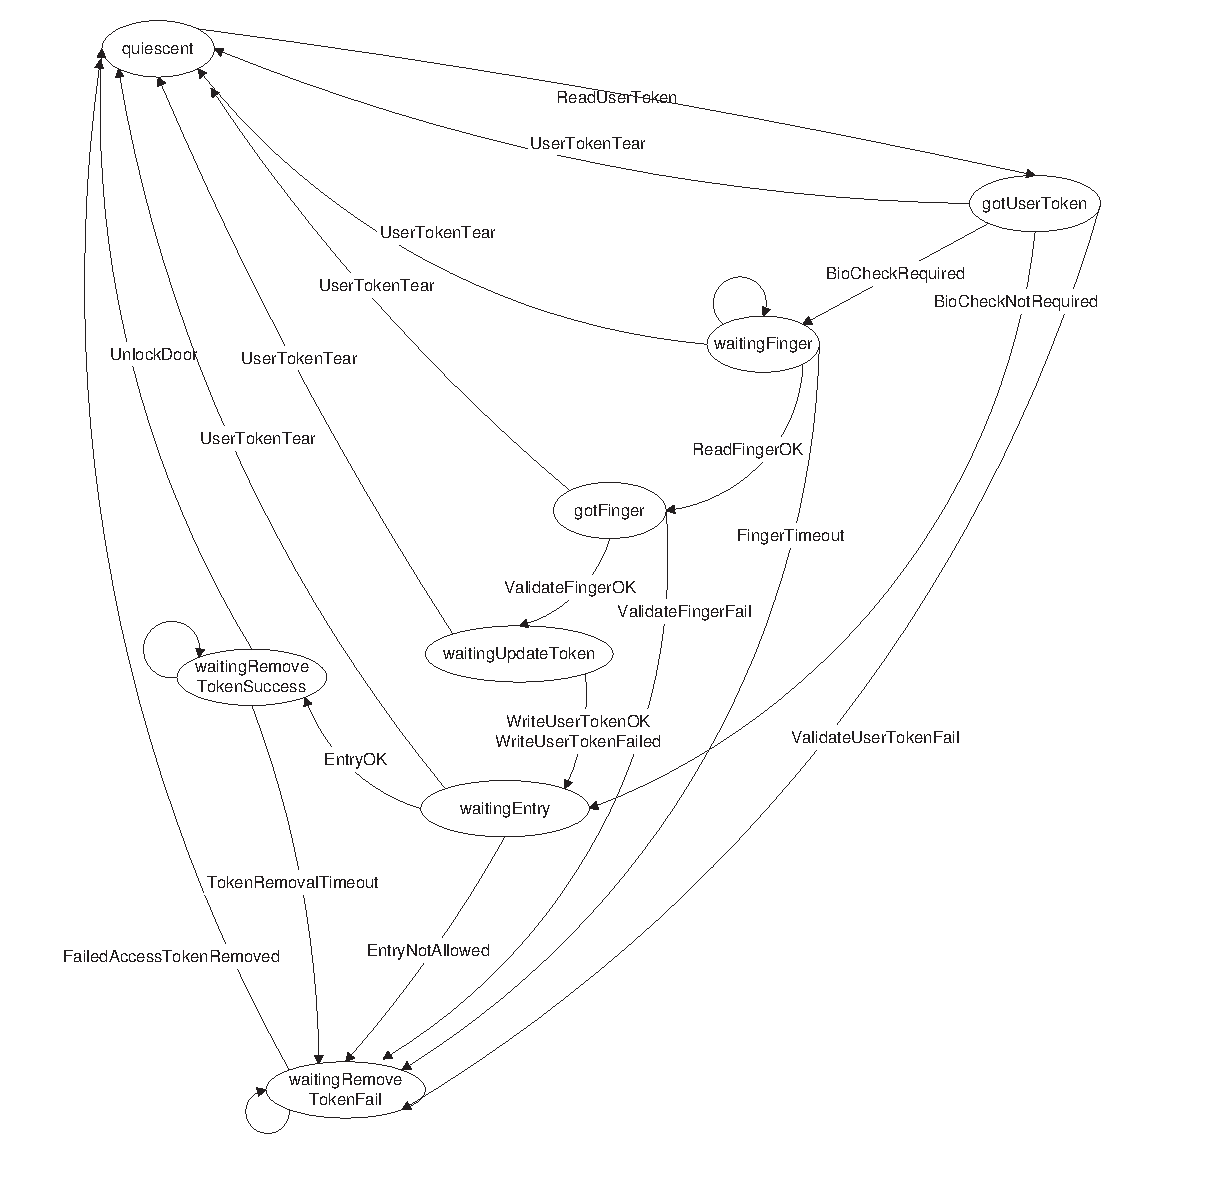
\includegraphics{41_2_entry.eps}}
    \caption{User Authentication and Entry state transitions}
    \label{fig:userEntry}
  \end{center}
\end{figure}

The process of user authentication and entry follows the following
stages:

\begin{itemize}
\item
Before any user attempts access, the system is $quiescent$.
\item
Once the token has been inserted and the information read off,
the status moves to $gotUserToken$, waiting for the system to validate
the token. 
\item
Once the token has been successfully validated the 
status moves to $waitingFinger$,
waiting for the user to give a fingerprint.
\item
Once the fingerprint has been read, the status moves to $gotFinger$,
waiting for the system to validate the fingerprint.
\item
Once a fingerprint has been successfully validated,
the status moves to $waitingUpdateToken$,
waiting to write the Auth Cert to the token.
\item
Once the Auth Cert has been written, the status moves to
$waitingEntry$, where it determines whether the role has
current entry privileges.
\item
If the role has current entry privileges the status moves to
$waitingTokenRemoveSuccess$, where the system waits for 
the token to be removed.
\item
Once the token has been removed
the latch will be unlocked if the role has current access privileges
to the enclave and the ID Station will return to $quiescent$.
\end{itemize}
In the case of a failure in the user validation process the status
moves to  $waitingRemoveTokenFail$, waiting until the token has been removed before returning to a
$quiescent$ state.

This specification separates opening the door from having a valid Auth
Certificate. It is possible for a role to be entitled to enter the
enclave but not use the workstations (for example such clearence might
be given to a buildings maintenance engineer). It is likely that TIS
configurations will ensure that having a valid Auth Certificate will
guarantee that entry to the enclave is permitted. 

\begin{traceunit}{FS.Enclave.ResetScreenMessage}
\end{traceunit}
The message displayed on the screen will indicate that the
system is busy while a user entry is in progress that blocks
administrator activity. Once the user entry activity becomes
non-blocking then an appropriate message is displayed on the screen.

\begin{schema}{ResetScreenMessage}
        \Delta Internal
\\      \Delta Admin
\\      currentScreen, currentScreen' : Screen
\where
        status' \notin \{ quiescent, waitingRemoveTokenFail \} 
\\ \t1 \land currentScreen'.screenMsg = busy
\\      \lor
\\      status' \in \{ quiescent, waitingRemoveTokenFail \}
\\ \t1 \land (enclaveStatus' = enclaveQuiescent \land rolePresent' = \Nil 
\\ \t3          \land currentScreen'.screenMsg = welcomeAdmin
\\ \t2 \lor enclaveStatus' = enclaveQuiescent \land rolePresent' \neq \Nil 
\\ \t3          \land currentScreen'.screenMsg = requestAdminOp
\\ \t2 \lor enclaveStatus' = waitingRemoveAdminTokenFail 
\\ \t3          \land currentScreen'.screenMsg = removeAdminToken
\\ \t2 \lor enclaveStatus' \notin 
        \{ enclaveQuiescent, waitingRemoveAdminTokenFail \} 
\\ \t3          \land currentScreen'.screenMsg = currentScreen.screenMsg)
\end{schema}

The user entry operation leaves much of the $IDStation$ state
unchanged. The context of this operation is summarised:

\begin{schema}{UserEntryContext}
        \Delta IDStation
\\      RealWorldChanges
\also
        \Xi Config
\\      \Xi AdminToken
\\      \Xi KeyStore
\\      \Xi Admin
\\      \Xi Keyboard
\\      \Xi Floppy
\\      \Xi Finger
\also
\\      \Xi TISControlledRealWorld
\also
\\      ResetScreenMessage
\where
        enclaveStatus' = enclaveStatus
\\      status \neq waitingEntry \implies tokenRemovalTimeout' = tokenRemovalTimeout
\end{schema} 

\begin{Zcomment}
\item
The following state components may change $UserToken$,
$DoorLatchAlarm$, $Stats$, $Internal$ and $AuditLog$.
\item
The components of the real world controlled by TIS remain unchanged.
\item
The $tokenRemovalTimeout$ is only updated if the current status is
$waitingEntry$.
\end{Zcomment}

Each of the following sub-operations is performed within the above context.

%----------------------------------------------------------------------
\section{User Token Tears}
%----------------------------------------------------------------------

\begin{traceunit}{FS.UserEntry.UserTokenTorn}
\traceto{ScGainInitial.Suc.Audit}
\traceto{ScGainInitial.Fail.ReadCard}
\traceto{ScProhibitInitial.Suc.Audit}
\traceto{ScProhibitInitial.Fail.ReadCard}
\traceto{ScGainRepeat.Suc.Audit}
\end{traceunit}


During the operation the user may tear his token from the reader
prematurely. There are a number of internal states during which token
removal is deamed erroneous.

If the user tears the Token out before the operation is complete then
the operation is terminated unsuccessfully.

\begin{schema}{UserTokenTorn}
        UserEntryContext
\also
	\Xi UserToken
\\      \Xi DoorLatchAlarm
\\      AddFailedEntryToStats
\also
        AddElementsToLog     
\where
        status \in \{ gotUserToken, waitingUpdateToken,
waitingFinger, gotFinger, waitingEntry \}
\\      userTokenPresence = absent
\also
        currentDisplay' = welcome
\\      status' = quiescent 
\end{schema}

%-------------------------------------------------------------------
\section{Reading the User Token}
%-------------------------------------------------------------------

\begin{traceunit}{FS.UserEntry.TISReadUserToken}
\traceto{ScGainInitial.Ass.Quiescent}
\traceto{ScGainInitial.Suc.Audit}
\traceto{ScGainInitial.Con.NoInterleave}
\traceto{ScProhibitInitial.Ass.Quiescent}
\traceto{ScProhibitInitial.Con.NoInterleave}
\traceto{ScProhibitInitial.Suc.Audit}
\traceto{ScGainRepeat.Ass.Quiescent}
\traceto{ScGainRepeat.Suc.Audit}
\traceto{ScGainRepeat.Con.NoInterleave}
\traceto{FIA\_UID.2.1}
\end{traceunit}

The User Entry operation is initiated when TIS is in a $quiescent$ state
and detects the presence of
a token in the user token reader (which resides outside the enclave). 

A user entry operation may start while the $enclaveStatus$ is
quiescent ($enclaveQuiescent$) or the enclave is waiting for a failed
admin token to be removed.

When the user token is first detected as present, its presence is
audited and the internal status changes. 
No other aspects of the system are modified.

\begin{schema}{ReadUserToken}
        UserEntryContext
\also
        \Xi UserToken
\\	\Xi DoorLatchAlarm
\\      \Xi Stats
\also
        AddElementsToLog
\where
        enclaveStatus \in \{ enclaveQuiescent,
        waitingRemoveAdminTokenFail \}
\also
	status = quiescent
\\	userTokenPresence = present
\also
	currentDisplay' = wait
\\	status' = gotUserToken
\end{schema}

The operation to read the user token is as follows:

\begin{zed}
        TISReadUserToken \defs  ReadUserToken
\end{zed}


%--------------------------------------------------------------------
\section{Validating the User Token}
%--------------------------------------------------------------------
Once TIS has read a user token it must validate the contents of that
token.

A user token is valid for entry into the enclave, without the need for
Biometric checks if the token contains an Authorisation certificate that
cross-checks correctly with the Token ID and the ID certificate, is
current and  both the Authorisation certificate and ID certificate can be
validated using the keys held in the TIS $KeyStore$. 

\begin{schema}{UserTokenWithOKAuthCert}
        KeyStore
\\      UserToken
\\      currentTime : TIME
\where
        currentUserToken \in \ran goodT
\\	\exists TokenWithValidAuth @ 
\\ \t1		(
		goodT(\theta TokenWithValidAuth) = currentUserToken
\\ \t1		\land currentTime \in (\The authCert).validityPeriod
\\ \t1          \land (\exists IDCert @ \theta IDCert = idCert \land CertOK )
\\ \t1          \land (\exists AuthCert @ \theta AuthCert = \The
authCert \land AuthCertOK )  
		)
\end{schema}



A user token is valid for entry into the enclave if the token is
consistent, current and the ID
certificate, Privilege certificate and I\&A certificate can be validated. This is regardless of the
presence or state of the Authorisation certificate. However in this
circumstance biometric checks will be required.

\begin{schema}{UserTokenOK}
        KeyStore
\\      UserToken
\\      currentTime : TIME
\where
 	currentUserToken \in \ran goodT
\\	\exists CurrentToken @ 
\\ \t1		(
		goodT(\theta ValidToken) = currentUserToken
\\ \t1		\land now = currentTime
\\ \t1          \land (\exists IDCert @ \theta IDCert = idCert \land CertOK )
\\ \t1          \land (\exists PrivCert @ \theta PrivCert = privCert
\land CertOK )
\\ \t1          \land (\exists IandACert @ \theta IandACert =
iandACert \land CertOK )  
                )
\end{schema}

\begin{traceunit}{FS.UserEntry.BioCheckNotRequired}
\traceto{ScGainInitial.Ass.GoodAC}
\traceto{ScGainRepeat.Suc.Audit}
\traceto{FCO\_NRO.2.1}
\traceto{FCO\_NRO.2.1}
\traceto{FCO\_NRO.2.3}
\traceto{FDP\_DAU.2.1}
\traceto{FDP\_DAU.2.2}
\end{traceunit}

In the case where there is a
valid Authorisation certificate the biometric checks are bypassed.

\begin{schema}{BioCheckNotRequired}
        UserEntryContext
\also
        \Xi UserToken
\\      \Xi DoorLatchAlarm        
\\      \Xi Stats
\also
        AddElementsToLog
\where
        status = gotUserToken
\\      userTokenPresence = present
\also
        UserTokenWithOKAuthCert
\also
        status' = waitingEntry
\\      currentDisplay' = wait
\end{schema}
\begin{Zcomment}
\item
The $userTokenValidElement$ is the audit entry recording that the
token has been succesfully validated.
\item 
The $authCertValidElement$ is the audit entry recording that the
token has a valid authorisation certificate.
\end{Zcomment}


\begin{traceunit}{FS.UserEntry.BioCheckRequired}
\traceto{ScGainInitial.Ass.ValidUser}
\traceto{ScGainInitial.Ass.PoorAC}
\traceto{ScGainInitial.Suc.Audit}
\traceto{FCO\_NRO.2.1}
\traceto{FCO\_NRO.2.1}
\traceto{FCO\_NRO.2.3}
\traceto{FDP\_DAU.2.1}
\traceto{FDP\_DAU.2.2}
\end{traceunit}


The biometric checks are only required if the Authorisation
Certificate is not present or not valid. In this case the remaining
certificates on the card must be checked.



\begin{schema}{BioCheckRequired}
        UserEntryContext
\also
        \Xi UserToken
\\      \Xi DoorLatchAlarm        
\\      \Xi Stats
\also
        AddElementsToLog
\where
        status = gotUserToken
\\      userTokenPresence = present
\also
        \lnot UserTokenWithOKAuthCert \land UserTokenOK
\also
	currentDisplay' = insertFinger
\\	status' = waitingFinger
\end{schema}


\begin{zed}
ValidateUserTokenOK \defs BioCheckRequired \lor BioCheckNotRequired
\end{zed}

\begin{traceunit}{FS.UserEntry.ValidateUserTokenFail}
\traceto{ScGainInitial.Fail.ReadCard}
\traceto{ScProhibitInitial.Ass.FalseUser}
\traceto{ScProhibitInitial.Ass.PoorAC}
\traceto{ScProhibitInitial.Suc.Audit}
\traceto{ScProhibitInitial.Fail.ReadCard}
\traceto{ScGainRepeat.Fail.ReadCard}
\end{traceunit}



There are lots of things that may go wrong with validation of the user
token. In each case the system will terminate the operation unsuccessfully.

\begin{schema}{ValidateUserTokenFail}
        UserEntryContext
\also
        \Xi UserToken
\\      \Xi DoorLatchAlarm
\\      \Xi Stats       
\also
        AddElementsToLog
\where
        status = gotUserToken
\\      userTokenPresence = present
\also
        \lnot UserTokenWithOKAuthCert \land \lnot UserTokenOK 
\also
        currentDisplay' = removeToken
\\      status' = waitingRemoveTokenFail
\end{schema}

\begin{zed}
        TISValidateUserToken \defs ValidateUserTokenOK \lor
        ValidateUserTokenFail 
\\ \t4 \lor
        [~UserTokenTorn | status = gotUserToken ]
\end{zed}

%-----------------------------------------------------------------
\section{Reading a fingerprint}
%----------------------------------------------------------------

\begin{traceunit}{FS.UserEntry.ReadFingerOK}
\traceto{ScGainInitial.Suc.Audit}
\traceto{ScProhibitInitial.Suc.Audit}
\end{traceunit}

A finger will be read if the system is currently waiting for it and
the user Token is in place.

\begin{schema}{ReadFingerOK}
        UserEntryContext
\also
        \Xi DoorLatchAlarm
\\	\Xi UserToken
\\      \Xi Stats
\also
        AddElementsToLog
\where
	status = waitingFinger
\\	fingerPresence = present
\\      userTokenPresence = present
\also
\\	currentDisplay' = wait
\\	status' = gotFinger
\end{schema}

\begin{traceunit}{FS.UserEntry.NoFinger}
\end{traceunit}


If there is no finger present then either nothing happens, since we
have not allowed sufficient attempts to get and validate a finger...

\begin{schema}{NoFinger}
        \Xi IDStation
\\      RealWorldChanges
\also
        \Xi TISControlledRealWorld
\where
        status = waitingFinger
\\      fingerPresence = absent
\\      userTokenPresence = present
\end{schema}


\begin{traceunit}{FS.UserEntry.FingerTimeout}
\traceto{ScGainInitial.Fail.Fingerprint}
\traceto{ScProhibitInitial.Suc.Audit}
\traceto{ScProhibitInitial.Fail.Fingerprint}
\end{traceunit}

...or TIS may have tried to obtain a valid finger for too
long, in which case the user is requested to remove the token and 
the operation is terminated unsuccessfully. Abstractly this  decision
is made non-deterministically.

\begin{schema}{FingerTimeout}
        UserEntryContext
\also
        \Xi UserToken
\\      \Xi DoorLatchAlarm
\\      \Xi Stats       
\also
        AddElementsToLog
\where
        status = waitingFinger
\\      userTokenPresence = present
\also
        currentDisplay' = removeToken
\\      status' = waitingRemoveTokenFail
\end{schema}

\begin{zed}
        TISReadFinger \defs ReadFingerOK \lor
        FingerTimeout \lor NoFinger 
\\ \t4  \lor [~ UserTokenTorn | status = waitingFinger ~]
\end{zed}

%-------------------------------------------------------------
\section{Validating a fingerprint}
%-------------------------------------------------------------

\begin{traceunit}{FS.UserEntry.ValidateFingerOK}
\traceto{ScGainInitial.Ass.ValidUser}
\traceto{ScGainInitial.Suc.Audit}
\end{traceunit}


A finger must match the template information extracted from the
userToken for it to be considered acceptable. The match criterion is
not modelled formally here athough it is necessary for the 
fingerprint to at least be good.

\begin{schema}{FingerOK}
        Finger
\\      UserToken
\where
        currentFinger \in \ran goodFP
\end{schema}

Within this specification the fingerprint will non-deterministically
match or not, assuming it is good.

The fingerprint being successfully validated is a prerequisite for
generating an authorisation certificate and adding it to the user token.
Validating the fingerprint is performed first.

\begin{schema}{ValidateFingerOK}
	UserEntryContext
\also
	\Xi DoorLatchAlarm
\\      \Xi UserToken
\also
        AddSuccessfulBioCheckToStats
\\      AddElementsToLog
\where
	status = gotFinger
\\      userTokenPresence = present
\also
        FingerOK
\also
	status' = waitingUpdateToken
\\	currentDisplay' = wait
\end{schema}


\begin{traceunit}{FS.UserEntry.ValidateFingerFail}
\traceto{ScGainInitial.Fail.Fingerprint}
\traceto{ScProhibitInitial.Ass.FalseUser}
\traceto{ScProhibitInitial.Suc.Audit}
\end{traceunit}


If the fingerprint is not successfully validated the user is asked to
remove their token and the entry attempt is terminated. 
The biometric check failure is recorded.

\begin{schema}{ValidateFingerFail}
        UserEntryContext
\also
	\Xi UserToken
\\      \Xi DoorLatchAlarm
\also      
        AddFailedBioCheckToStats
\\      AddElementsToLog
\where
        status = gotFinger
\\      userTokenPresence = present
\also
        currentDisplay' = removeToken
\\      status' = waitingRemoveTokenFail
\end{schema}

\begin{zed}
        TISValidateFinger \defs ValidateFingerOK \lor ValidateFingerFail
\\ \t4  \lor [~ UserTokenTorn | status = gotFinger ~]
\end{zed}

%---------------------------------------------------------------------
\section{Writing the User Token}
%----------------------------------------------------------------------


\begin{traceunit}{FS.UserEntry.WriteUserTokenOK}
\traceto{ScGainInitial.Suc.GoodAC}
\traceto{ScGainInitial.Suc.PersistCerts}
\traceto{ScGainInitial.Suc.Audit}
\end{traceunit}

An attempt is made to write this certificate to the token. The write of
the authorisation certificate may be successful...

\begin{schema}{WriteUserTokenOK}
	UserEntryContext
\also
	\Xi DoorLatchAlarm
\\      \Xi Stats
\also
        AddElementsToLog
\\      AddAuthCertToUserToken
\where
	status = waitingUpdateToken
\\      userTokenPresence = present
\also
        status' = waitingEntry
\\      currentDisplay' = wait
\end{schema}


\begin{traceunit}{FS.UserEntry.WriteUserTokenFail}
\traceto{ScGainInitial.Fail.WriteCard}
\end{traceunit}

... or may fail. The failure case models circumstances where the TIS
can detect the failure, through a write failure for instance. 
As there is no read back of the authorisation certificate we cannot
guarantee that the audit log indicating a successful write means that
the token contains the authorisation certificate. The user will still
subsequently be admitted to the enclave if the conditions are correct. 

\begin{schema}{WriteUserTokenFail}
	UserEntryContext
\also
	\Xi DoorLatchAlarm
\\      \Xi Stats
\also
        AddElementsToLog
\\      AddAuthCertToUserToken
\where
	status = waitingUpdateToken
\\      userTokenPresence = present
\also
        status' = waitingEntry
\\      currentDisplay' = tokenUpdateFailed
\end{schema}


Abstractly, whether the authorisation certificate is successfully
written or not is non-deterministic.   

The failure will actually happen during the physical write to the
token, during $UpdateUserToken$. However, as the
operations $WriteUserToken$ and $UpdateUserToken$ are both used to
build the atomic operation $TISWriteUserToken$, the non-deterministic 
failure still happens sometime within this atomic operation.

\begin{zed}
WriteUserToken \defs WriteUserTokenOK \lor WriteUserTokenFail
\end{zed}

\begin{zed}
        TISWriteUserToken \defs (
        WriteUserToken \semi UpdateUserToken )
\\ \t4          \lor [~ UserTokenTorn | status = waitingUpdateToken ~] 
\end{zed}



%------------------------------------------------------------
\section{Validating Entry}
%------------------------------------------------------------

The door will only be unlocked if the current TIS configuration allows
the user to enter the enclave at this time. It is likely that TIS
configurations will ensure that having a valid Auth Certificate will
guarantee that entry to the enclave is permitted, but such a
constraint is not specified here. 

TIS checks to ensure that the current configuration allows the user to
enter the enclave:


\begin{schema}{UserAllowedEntry}
        UserToken
\\      Config
\\      currentTime: TIME
\where
        (\exists ValidToken @ 
\\ \t1  goodT (\theta ValidToken) = currentUserToken
\\ \t1  \land currentTime \in entryPeriod~ privCert.role~
privCert.clearance.class )
\\ \lor
        (\exists TokenWithValidAuth @ 
\\ \t1 goodT(\theta TokenWithValidAuth) = currentUserToken 
\\ \t1 \land currentTime \in entryPeriod~
        (\The authCert).role~ (\The authCert).clearance.class)
\end{schema}


\begin{traceunit}{FS.UserEntry.EntryOK}
\end{traceunit}


Only if entry is permitted at the current time will the user be
admitted to the enclave.

\begin{schema}{EntryOK}
        UserEntryContext
\also
        \Xi DoorLatchAlarm
\\      \Xi UserToken
\\      \Xi Stats
\also
        AddElementsToLog
\where
        status = waitingEntry
\\      userTokenPresence = present
\also
        UserAllowedEntry
\also
        currentDisplay' = openDoor
\\      status' = waitingRemoveTokenSuccess
\\      tokenRemovalTimeout' = currentTime + tokenRemovalDuration
\end{schema}

\begin{traceunit}{FS.UserEntry.EntryNotAllowed}
\end{traceunit}

If the user is not allowed entry at this time they will be
requested to remove their token.

\begin{schema}{EntryNotAllowed}
        UserEntryContext
\also
        \Xi DoorLatchAlarm
\\      \Xi UserToken
\\      \Xi Stats       
\also
        AddElementsToLog
\where
        status = waitingEntry
\\      userTokenPresence = present
\also
        \lnot UserAllowedEntry
\also
        currentDisplay' = removeToken
\\      status' = waitingRemoveTokenFail
\\      tokenRemovalTimeout' = tokenRemovalTimeout
\end{schema}

\begin{zed}
        TISValidateEntry \defs EntryOK
\\ \t4          \lor EntryNotAllowed
\\ \t4          \lor [~ UserTokenTorn | status = waitingEntry ~] 
\end{zed}


%------------------------------------------------------------
\section{Unlocking the Door}
%------------------------------------------------------------

\begin{traceunit}{FS.UserEntry.UnlockDoorOK}
\traceto{ScGainInitial.Suc.UserCard}
\traceto{ScGainInitial.Suc.UserIn}
\traceto{ScGainInitial.Suc.Audit}
\traceto{ScGainRepeat.Suc.UserCard}
\traceto{ScGainRepeat.Suc.UserIn}
\traceto{ScGainRepeat.Suc.Audit}
\end{traceunit}


The door will only be unlocked once the user has removed their token.
This helps remind the user to take their token with them.

\begin{schema}{UnlockDoorOK}
        UserEntryContext
\also
      \Xi UserToken
\also
        UnlockDoor
\\      AddSuccessfulEntryToStats
\\      AddElementsToLog
\where
        status = waitingRemoveTokenSuccess
\\      userTokenPresence = absent
\also
        currentDisplay' = doorUnlocked
\\      status' = quiescent
\end{schema}

\begin{traceunit}{FS.UserEntry.WaitingTokenRemoval}
\end{traceunit}

The system will wait indefinitely for a token to be removed, however
the system will deny entry to a user who takes too long to extract
their token.

\begin{schema}{WaitingTokenRemoval}
        \Xi IDStation
\\      RealWorldChanges
\also
        \Xi TISControlledRealWorld
\where
        status \in \{ waitingRemoveTokenSuccess, 
waitingRemoveTokenFail \}
\\      status = waitingRemoveTokenSuccess \implies currentTime \leq tokenRemovalTimeout 
\\      userTokenPresence = present
\end{schema}

\begin{traceunit}{FS.UserEntry.TokenRemovalTimeout}
\end{traceunit}

If the user waits too long to remove their token then this is logged
and the system continues to wait for the token to be removed but will
no longer allow access to the enclave.

\begin{schema}{TokenRemovalTimeout}
        UserEntryContext
\also
        \Xi DoorLatchAlarm
\\      \Xi UserToken
\\      \Xi Stats       
\also
        AddElementsToLog
\where
        status = waitingRemoveTokenSuccess
\\      currentTime > tokenRemovalTimeout 
\\      userTokenPresence = present
\also
        status' = waitingRemoveTokenFail
\\      currentDisplay' = removeToken
\end{schema}


\begin{zed}
        TISUnlockDoor \defs UnlockDoorOK 
\\      \t2 \lor [ WaitingTokenRemoval |status =
waitingRemoveTokenSuccess ]
\\      \t2 \lor TokenRemovalTimeout
\end{zed}
 
%------------------------------------------
\section{Terminating a failed access}
%------------------------------------------

\begin{traceunit}{FS.UserEntry.FailedAccessTokenRemoved}
\traceto{ScGainInitial.Suc.Audit}
\traceto{ScProhibitInitial.Suc.UserCard}
\traceto{ScProhibitInitial.Suc.Audit}
\end{traceunit}

If an access attempt has failed the system waits for the token to be
removed before a new user entry operation can commence. Once the token has been
removed a new user entry may start.

The operations in the enclave are not blocked on the presence of a
failed user token in the token reader. 

\begin{schema}{FailedAccessTokenRemoved}
        UserEntryContext
\also
	\Xi UserToken
\\      \Xi DoorLatchAlarm
\also
        AddFailedEntryToStats
\\      AddElementsToLog
\where
        status = waitingRemoveTokenFail
\\      userTokenPresence = absent
\also
        currentDisplay' = welcome
\\      status' = quiescent
\end{schema}

\begin{zed}
        TISCompleteFailedAccess \defs FailedAccessTokenRemoved 
\\      \t2     \lor [ WaitingTokenRemoval | status = waitingRemoveTokenFail ] 
\end{zed}

%..........................................
\section{The Complete User Entry}
%..........................................

\begin{traceunit}{FS.UserEntry.TISUserEntryOp}
\traceto{FIA\_UAU.7.1}
\end{traceunit}

The complete authentication process, triggered by TIS reading a User
Token, involves validating the user Token, reading and validating the
fingerprint, 
writing an authorisation certificate to the user token, waiting for
the user to remove the token, opening the door to the enclave and
in the case of a failure waiting for the system to
be in a state where it can admit another user.

\begin{zed}
        TISUserEntryOp \defs TISReadUserToken \lor TISValidateUserToken \lor TISReadFinger \lor
                TISValidateFinger 
\\ \t4          \lor TISWriteUserToken \lor  TISValidateEntry \lor TISUnlockDoor \lor
                TISCompleteFailedAccess 
\end{zed}





%====================================================================
\chapter{Operations Within the Enclave}
\label{sec:Enclave}
%====================================================================

A number of interactions with TIS may occur within the
Enclave.
These interactions leave some of the $IDStation$ state unchanged.

\begin{schema}{EnclaveContext}
        \Delta IDStation
\\      RealWorldChanges
\also
        \Xi TISControlledRealWorld
\also
        \Xi UserToken
\\      \Xi AdminToken
\\      \Xi Finger
\\      \Xi Stats
\where
        tokenRemovalTimeout' = tokenRemovalTimeout
\end{schema}
\begin{Zcomment}
\item
The following state components may change $KeyStore$, 
$Floppy$, $Config$, $Admin$, $Keyboard$,
$DoorLatchAlarm$, $Internal$ and $AuditLog$. 
\item
The components of the real world controlled by TIS remain unchanged.
\end{Zcomment}

The operations that may occur within the enclave include
administrator operations and the ID station enrolment. These are
described in this section.

%-------------------------------------------------------------------------
\section{Enrolment of an ID Station}
%-------------------------------------------------------------------------

\begin{traceunit}{FS.Enclave.TISEnrolOp}
\end{traceunit}

Before TIS can be used it must be enrolled.

We assume
that the initial enrolment is the only possible enrolment activity.

Enrolment is a multi-phase activity, the state transistions for an
enrolment are given in Figure \ref{fig:enrol}. Before enrolment the
system is in state $notEnrolled$ and, on successful completion, it
enters the $quiescent$ state.

\begin{figure}[htbp]
  \begin{center}
    \leavevmode
    \resizebox{\textwidth}{!}{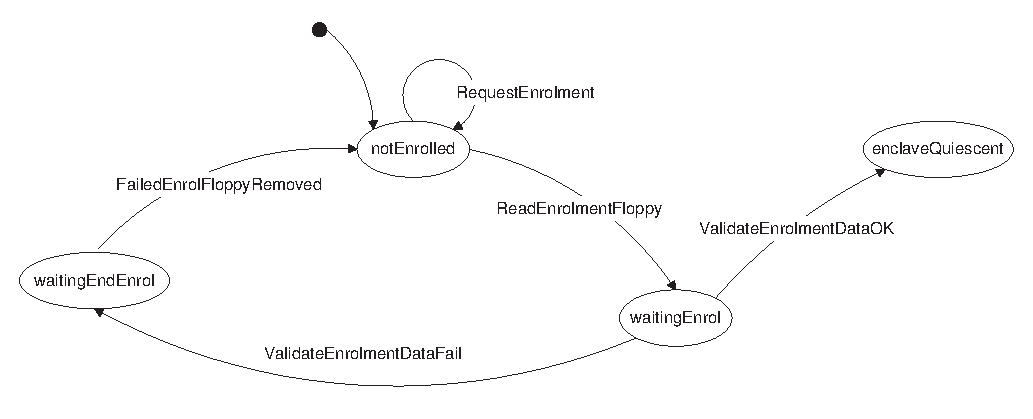
\includegraphics{41_2_enrol.eps}}
    \caption{Enrolment state transitions}
    \label{fig:enrol}
  \end{center}
\end{figure}

The context for all enrolment operations is given below.

\begin{schema}{EnrolContext}
        EnclaveContext
\also
        \Xi Keyboard
\\      \Xi Admin
\\      \Xi DoorLatchAlarm
\\      \Xi Config
\\      \Xi Floppy
\end{schema}

\begin{Zcomment}
\item
The following state components may change
$KeyStore$, $Internal$ and $AuditLog$. 
\end{Zcomment}


%...................................
\subsection{Requesting Enrolment}
%...................................

\begin{traceunit}{FS.Enclave.RequestEnrolment}
\end{traceunit}


The ID station will request enrolment while there is no Floppy
present. This will occur until a successful enrolment is achieved.

\begin{schema}{RequestEnrolment}
        EnrolContext
\also
        \Xi KeyStore
\\      \Xi AuditLog
\\      \Xi Internal
\where
        enclaveStatus = notEnrolled
\\      floppyPresence = absent
\also
        currentScreen'.screenMsg = insertEnrolmentData
\also
        currentDisplay' = blank
\end{schema}

\begin{traceunit}{FS.Enclave.ReadEnrolmentFloppy}
\traceto{ScStart.Ass.Data}
\traceto{ScStart.Con.NoInterleave}
\end{traceunit}

If a floppy is present then TIS goes on to validate the
contents. Nothing is written to the log at this stage as log entries
will be made on successful or failed enrolment.

\begin{schema}{ReadEnrolmentFloppy}
        EnrolContext
\also
        \Xi KeyStore
\where
        enclaveStatus = notEnrolled
\\      floppyPresence = present
\also
        currentScreen'.screenMsg = validatingEnrolmentData 
\also
        enclaveStatus' = waitingEnrol     
\\      status' = status
\\      currentDisplay' = blank                         
\end{schema}

\begin{zed}
        ReadEnrolmentData \defs ReadEnrolmentFloppy \lor RequestEnrolment
\end{zed}

%.........................................
\subsection{Validating Enrolment data from Floppy}
%.........................................

For the enrolment data to be acceptable the data on the floppy must be
valid enrolment data with the ID Station certificate containing this
ID station's public key. 

\begin{schema}{EnrolmentDataOK}
        Floppy
\\      KeyStore
\where
        currentFloppy \in \ran enrolmentFile
\\      (\exists ValidEnrol @ \theta ValidEnrol = enrolmentFile \inv
currentFloppy)
\end{schema}

\begin{traceunit}{FS.Enclave.ValidateEnrolmentDataOK}
\traceto{ScStart.Suc.Running}
\traceto{ScStart.Suc.Audit}
\traceto{FMT\_MSA.2.1}
\traceto{FMT\_MTD.3.1}
\end{traceunit}


If the data on the floppy is acceptable to be used for enrolment then
the Key store is updated. From this point the system is available for
use both by users entering the enclave and by administrators.

\begin{schema}{ValidateEnrolmentDataOK}
        EnrolContext
\also
        UpdateKeyStoreFromFloppy
\\      AddElementsToLog
\where
        enclaveStatus = waitingEnrol
\also
        EnrolmentDataOK
\also
        currentScreen'.screenMsg = welcomeAdmin
\also
        enclaveStatus' = enclaveQuiescent 
\\      status' = quiescent
\\      currentDisplay' = welcome
\end{schema}

\begin{traceunit}{FS.Enclave.ValidateEnrolmentDataFail}
\traceto{ScStart.Fail.ReadFloppy}
\end{traceunit}

If the enrolment fails then TIS waits for the floppy to be removed
before prompting for new enrolment data. 

\begin{schema}{ValidateEnrolmentDataFail}
        EnrolContext
\also
        \Xi KeyStore
\also
        AddElementsToLog
\where
        enclaveStatus = waitingEnrol
\also
        \lnot EnrolmentDataOK
\also
        currentScreen'.screenMsg = enrolmentFailed
\also
        enclaveStatus' = waitingEndEnrol
\\      status' = status
\\      currentDisplay' = blank
\end{schema}

\begin{zed}
        ValidateEnrolmentData \defs ValidateEnrolmentDataOK \lor
          ValidateEnrolmentDataFail
\end{zed}

%.........................................
\subsection{Completing a failed Enrolment}
%.........................................

A failed enrolment will only terminate once the floppy has been
removed, otherwise the system would repeatedly try to validate the
same floppy.

\begin{traceunit}{FS.Enclave.FailedEnrolFloppyRemoved}
\end{traceunit}


Once the floppy has been removed the administrator is prompted for
enrolment data again. We do not log the removal of the floppy in the
audit log.

\begin{schema}{FailedEnrolFloppyRemoved}
        EnrolContext
\also
        \Xi KeyStore
\where
        enclaveStatus = waitingEndEnrol
\\      floppyPresence = absent
\also
        currentScreen'.screenMsg = insertEnrolmentData
\also
        enclaveStatus' = notEnrolled
\\      status' = status
\\      currentDisplay' = blank
\end{schema}

\begin{traceunit}{FS.Enclave.WaitingFloppyRemoval}
\end{traceunit}

TIS will wait indefinately for the floppy to be removed after an
unsuccessful enrolment, this is because enrolment is triggered by the
presence of the floppy alone.

\begin{schema}{WaitingFloppyRemoval}
        EnclaveContext
\also
        \Xi IDStation
\where
        enclaveStatus = waitingEndEnrol
\\      floppyPresence = present
\end{schema}

\begin{zed}
        CompleteFailedEnrolment \defs FailedEnrolFloppyRemoved  
         \lor WaitingFloppyRemoval
\end{zed}

%..........................................
\subsection{The Complete Enrolment}
%..........................................

The complete enrolment process involves reading the enrolment data,
validating it and, in the case of a failure waiting for the system to
be in a state where it can try another enrolment.

\begin{zed}
        TISEnrolOp \defs ReadEnrolmentData \lor
ValidateEnrolmentData 
\\      \t4 \lor CompleteFailedEnrolment
\end{zed}

%-----------------------------------------------------------------------
\section{Administrator Token Tear}
%-----------------------------------------------------------------------

The action of removing the administrator Token will result in the
administrator being logged out of the system.

This may happen at any point once a token has been inserted into the
reader. As soon as the adminitrator's token is torn this action will
be logged. The screen message will be reset if the system is not busy
with processing a user entry.

\begin{schema}{AdminTokenTear}
         EnclaveContext
\also
        \Xi Config
\\      \Xi Floppy
\\      \Xi Keyboard
\\      \Xi DoorLatchAlarm
\\      \Xi KeyStore
\\      ResetScreenMessage
\where
        adminTokenPresence = absent
\also   
        status' = status
\\      currentDisplay' = currentDisplay
\also
        enclaveStatus' = enclaveQuiescent
\end{schema}

If the admin token is torn while the system is processing an activity
within the enclave then the activity will be stopped.

\begin{schema}{BadAdminTokenTear} 
        AdminTokenTear
\also
        AddElementsToLog
\where
        enclaveStatus \in \{gotAdminToken, waitingStartAdminOp, waitingFinishAdminOp \}
\end{schema}

\begin{traceunit}{FS.Enclave.BadAdminLogout}
\traceto{ScLogOff.Ass.LoggedOn}
\traceto{ScLogOff.Suc.LoggedOff}
\traceto{ScLogOff.Suc.Audit}
\end{traceunit}

If the administrator is performing an operation when the token is torn
then the administrator will be logged off.

\begin{schema}{BadAdminLogout}
        BadAdminTokenTear
\\      AdminLogout
\where
        enclaveStatus \in \{ waitingStartAdminOp, waitingFinishAdminOp
        \}
\end{schema}


\begin{traceunit}{FS.Enclave.LoginAborted}
\end{traceunit}

If the token is torn during the log on validation process then there
is no need to log off the administrator.

\begin{schema}{LoginAborted}
        BadAdminTokenTear
\\      \Xi Admin
\where
        enclaveStatus = gotAdminToken
\end{schema}


%----------------------------------------------------------------------
\section{Administrator Login}
%----------------------------------------------------------------------


An Administrator logs into TIS by inserting a valid token
into the $adminToken$ reader. The authorisation certificate is
verified and the user is logged in with the privileges indicated on
the card.

Once the administrator is successfully logged into TIS, the system
records that there is a role present. The process of logging on is
given by the state transition diagram in Figure \ref{fig:logon}

\begin{figure}[htbp]
  \begin{center}
    \leavevmode
    \resizebox{\textwidth}{!}{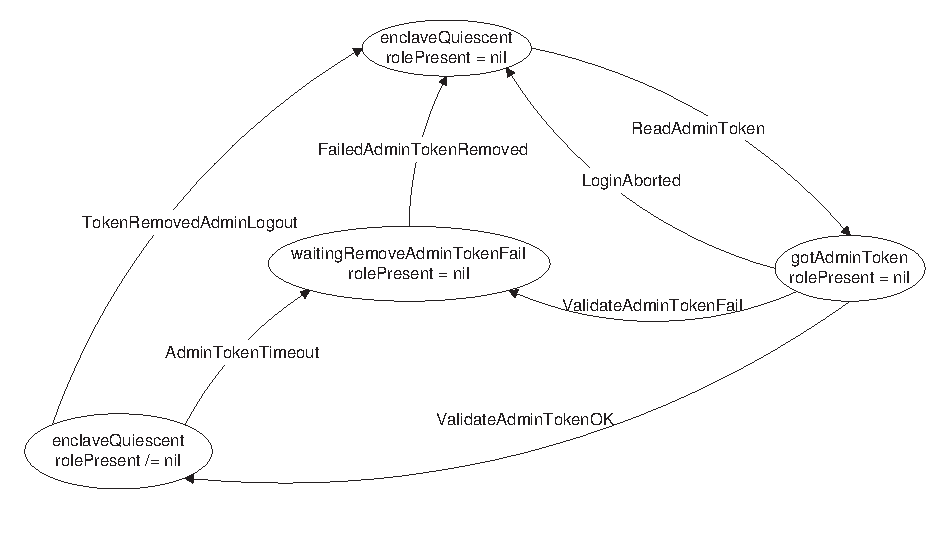
\includegraphics{41_2_admin.eps}}
    \caption{Administrator logon/logoff state transitions}
    \label{fig:logon}
  \end{center}
\end{figure}

The context for administrator login is given below.

\begin{schema}{LoginContext}
        EnclaveContext
\also
        \Xi Keyboard
\\      \Xi KeyStore
\\      \Xi DoorLatchAlarm
\\      \Xi Config
\\      \Xi Floppy
\where
        status' = status
\\      currentDisplay' = currentDisplay
\end{schema}

\begin{Zcomment}
\item
The following state components may change
$Admin$, $Internal$ and $AuditLog$. 
\end{Zcomment}

%..........................................
\subsection{Read Administrator Token}
%..........................................

\begin{traceunit}{FS.Enclave.ReadAdminToken}
\traceto{ScLogOn.Ass.Quiescent}
\traceto{ScLogOn.Suc.Audit}
\traceto{ScLogOn.Con.NoInterleave}
\traceto{FIA\_UID.2.1}
\traceto{FMT\_SMR.3.1}
\end{traceunit}

When the admin token is read the action is audited and the internal
status changes. No other aspects of the system are modified.

An administrator can only log on when there is no user entry activity
in progress or TIS is waiting for a failed user token to be removed
from the token reader outside of the enclave.

\begin{schema}{ReadAdminToken}
         LoginContext
\also
        \Xi Admin
\also
        AddElementsToLog
\where
        status \in \{~ quiescent, waitingRemoveTokenFail ~\}
\also
        enclaveStatus = enclaveQuiescent
\\      rolePresent = \Nil
\\	adminTokenPresence = present
\also
	enclaveStatus' = gotAdminToken
\\      currentScreen' = currentScreen
\end{schema}

The operation to read the token is as follows:

\begin{zed}
        TISReadAdminToken \defs 
                ReadAdminToken   
\end{zed}

%..........................................
\subsection{Validate Administrator Token}
%..........................................

An administrator's token is considered valid if it cotains a current
authorisation certificate that correctly cross references to the token
ID and the ID certificate and both these certificates can be validated
using the keys held in the $KeyStore$. Additionally the
privileges assigned to the user within the authorisation certificate
must indicate that the user is actually an administrator.

\begin{schema}{AdminTokenOK}
        AdminToken
\\      KeyStore
\\      currentTime : TIME        
\where
        currentAdminToken \in \ran goodT
\also
        \exists TokenWithValidAuth @
\\ \t1  (goodT(\theta TokenWithValidAuth )  = currentAdminToken
\\ \t1  \land (\exists IDCert @ \theta IDCert = idCert \land CertOK )
\\ \t1  \land (\exists AuthCert @ \theta AuthCert = \The authCert \land
AuthCertOK )
\\ \t1  \land (\The authCert).role \in ADMINPRIVILEGE 
\\ \t1  \land currentTime \in (\The authCert).validityPeriod)
\end{schema}
\begin{Zcomment}
\item
Only the $AuthCert$  and $IDCert$ are checked at this point. The remaining
certificates were checked on entry to the enclave.
\item
The Token must indicate that the user has an administrator privilege.
\end{Zcomment}

\begin{traceunit}{FS.Enclave.ValidateAdminTokenOK}
\traceto{ScLogOn.Ass.ValidAdmin}
\traceto{ScLogOn.Suc.LogOn}
\traceto{ScLogOn.Suc.Audit}
\traceto{SFP.DAC}
\traceto{FCO\_NRO.2.1}
\traceto{FCO\_NRO.2.2}
\traceto{FCO\_NRO.2.3}
\traceto{FDP\_ACC.1.1}
\traceto{FDP\_ACF.1.1}
\traceto{FDP\_ACF.1.2}
\traceto{FDP\_ACF.1.3}
\traceto{FDP\_ACF.1.4}
\traceto{FIA\_USB.1.1}
\traceto{FMT\_MSA.1.1}
\traceto{FMT\_MTD.1.1}
\traceto{FMT\_SAE.1.1}
\traceto{FMT\_SMR.2.1}
\traceto{FMT\_SMR.2.2}
\end{traceunit}


If the token can be validated then the administrator is logged onto
TIS.

\begin{schema}{ValidateAdminTokenOK}
        LoginContext
\also
        AdminLogon
\also
        AddElementsToLog
\where
        enclaveStatus = gotAdminToken
\\      adminTokenPresence = present
\also
        AdminTokenOK
\also   
        currentScreen'.screenMsg = requestAdminOp 
\also
        enclaveStatus' = enclaveQuiescent
\end{schema}

\begin{traceunit}{FS.Enclave.ValidateAdminTokenFail}
\traceto{ScLogOn.Fail.ReadCard}
\end{traceunit}

If the token can not be validated then TIS waits for it to be removed.

\begin{schema}{ValidateAdminTokenFail}
        LoginContext
\also
        \Xi Admin
\also
        AddElementsToLog
\where
        enclaveStatus = gotAdminToken
\\      adminTokenPresence = present
\also
        \lnot AdminTokenOK
\also
        currentScreen'.screenMsg = removeAdminToken
\also
        enclaveStatus' = waitingRemoveAdminTokenFail
\end{schema}

\begin{zed}
        TISValidateAdminToken \defs ValidateAdminTokenOK \lor
        ValidateAdminTokenFail 
\\ \t4  \lor
        LoginAborted
\end{zed}

\subsection{Complete Failed Administrator Logon}

If an administrator token has failed to be accepted by TIS 
then no further actions can take place in the enclave until it has 
been removed.

\begin{traceunit}{FS.Enclave.FailedAdminTokenRemoved}
\end{traceunit}


The administrator token may be removed at any point during a user
entry, hence the context for this
activity does not place restrictions on the value of $status$.

When the admin token is removed TIS returns to a state ready
to accept another administrator logon.
\begin{schema}{FailedAdminTokenRemoved}
        LoginContext
\also
        \Xi Admin
\also 
        AddElementsToLog
\where
        enclaveStatus = waitingRemoveAdminTokenFail
\\      adminTokenPresence = absent
\also
        currentScreen'.screenMsg = welcomeAdmin
\also
        enclaveStatus' = enclaveQuiescent
\also
        currentDisplay' = currentDisplay
\end{schema}

\begin{traceunit}{FS.Enclave.WaitingAdminTokenRemoval}
\end{traceunit}


TIS will wait indefinitely for the Admin Token to be removed after a
failed attempt to logon.

\begin{schema}{WaitingAdminTokenRemoval}
        EnclaveContext
\also
        \Xi IDStation
\where
        enclaveStatus = waitingRemoveAdminTokenFail
\\      adminTokenPresence = present     
\end{schema}

\begin{zed}
        TISCompleteFailedAdminLogon \defs FailedAdminTokenRemoved 
\lor WaitingAdminTokenRemoval
\end{zed}

\subsection{The Complete Administrator Logon}

\begin{traceunit}{FS.Enclave.TISAdminLogin}
\end{traceunit}

The complete administrator logon process, from the point that the
system has detected the presence of a token in the administrator
reader, involves 
validating the administrator token and, in the case of a failure 
waiting for the system to be in a state where it can try another logon.

\begin{zed}
        TISAdminLogon \defs TISReadAdminToken \lor TISValidateAdminToken \lor TISCompleteFailedAdminLogon
\end{zed}

%-----------------------------------------------------------------
\section{Administrator Logout}
%-----------------------------------------------------------------

Administrator logout can be achieved in two ways, either the
administrator removes their token from TIS, or the Authorisation
certificate on the token expires, causing the system to automatically
log off the administrator.

\begin{traceunit}{FS.Enclave.AdminLogout}
\traceto{ScLogOff.Ass.LoggedOn}
\traceto{ScLogOff.Suc.LoggedOff}
\traceto{ScLogOff.Suc.Audit}
\end{traceunit}

If TIS is not performing an administrator operation then the
token may be removed to log out the administrator.

\begin{schema}{TokenRemovedAdminLogout}
        AdminTokenTear
\\      AdminLogout
\also
        AddElementsToLog
\where
        enclaveStatus = enclaveQuiescent 
\\      rolePresent \neq \Nil
\end{schema}

\begin{traceunit}{FS.Enclave.AdminTokenTimeout}
\end{traceunit}


The TIS will automatically logout an administrator whose token
expires. This occurs if the validity period on the Authorisation
certificate expires.

\begin{schema}{AdminTokenTimeout}
        LoginContext
\also
        AdminLogout
\\      AddElementsToLog
\\      ResetScreenMessage
\where
        enclaveStatus = enclaveQuiescent 
\\      adminTokenPresence = present
\\      rolePresent \neq \Nil
\also
        \lnot AdminTokenOK
\also
        enclaveStatus' = waitingRemoveAdminTokenFail
\end{schema}

\begin{traceunit}{FS.Enclave.TISCompleteTimeoutAdminLogout}
\end{traceunit}

If the administrator's token expires then it must be removed before
further activities can take place at the TIS console. This behaviour
is identical to the behaviour when the system waits for a the
administrator to remove their token following a failed logon.

\begin{zed}
TISCompleteTimeoutAdminLogout \defs TISCompleteFailedAdminLogon
\end{zed}

%...........................
\subsection{Complete Administrator Logout}
%............................

\begin{traceunit}{FS.Enclave.TISAdminLogout}
\end{traceunit}

THe complete administrator logout process, from the point that it
decides to log out an administrator to the point that it is in a state
where it can try another logon is givien below.

\begin{zed}
TISAdminLogout \defs  TokenRemovedAdminLogout \lor AdminTokenTimeout \lor TISCompleteTimeoutAdminLogout 
\end{zed}

%-----------------------------------------------------------------
\section{Administrator Operations}
%-----------------------------------------------------------------
An administrator operation can take place as long as an administrator
is present. The operation is started by receiving a valid request to
perform an operation from the keyboard. TIS will ensure that the
requested operation is one compatible with the current role present.

Once the operation is started the behaviour depends on the type of
operation. Operations are either short, and can be implemented in one
phase or they are multi-phase operations. 

$shutdown$ and $overrideLock$ are short operations, while $archiveLog$
and $updateCofigData$ are multi phase operations.

The state transition diagram for administrator operations is given in
Figure \ref{fig:adminOp}

\begin{figure}[htbp]
  \begin{center}
    \leavevmode
    \resizebox{\textwidth}{!}{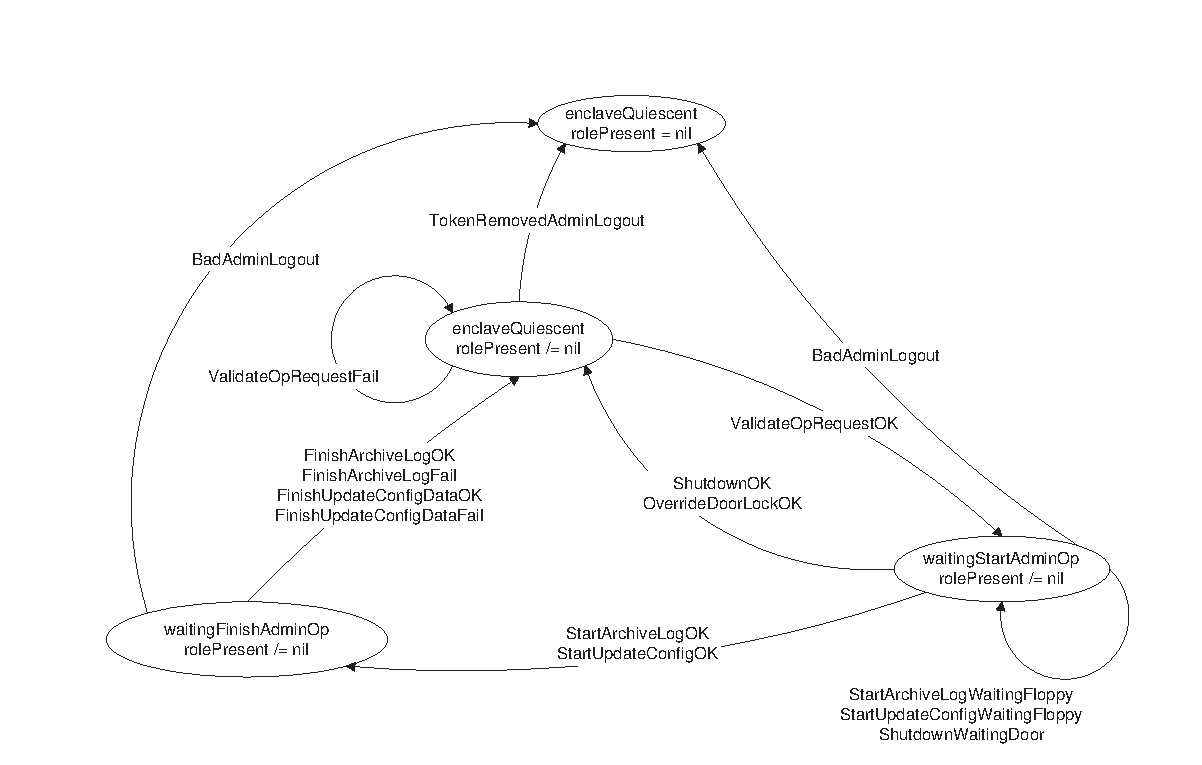
\includegraphics{41_2_adminOp.eps}}
    \caption{Administrator operation state transitions}
    \label{fig:adminOp}
  \end{center}
\end{figure}

All administrator operations have a common context, in which the
$AdminToken$ does not change.
An administrator can only perform an operation when there is no user 
entry activity
in progress or TIS is waiting for a failed user token to be removed
from the token reader outside of the enclave.


\begin{schema}{AdminOpContext}
        EnclaveContext
\also
        \Xi Keyboard
\\      \Xi KeyStore
\end{schema}
\begin{Zcomment}
\item
The following state components may change   
$Floppy$, $Config$, $Admin$, $DoorLatchAlarm$, $Internal$ and $AuditLog$. 
\end{Zcomment}

Once an operation has been started its context is given by:

\begin{schema}{AdminOpStartedContext}
        AdminOpContext
\where
        enclaveStatus = waitingStartAdminOp
\\      adminTokenPresence = present
\also
        status' = status
\end{schema}
\begin{Zcomment}
\item
The $adminToken$ will be present, its removal is erroneous.
\item
The system has a record of the name of the current operation.
\end{Zcomment}

Some operations are multi-phase, the context for completing a
multi-phase operation is given by: 

\begin{schema}{AdminOpFinishContext}
        AdminOpContext
\also
        AdminFinishOp
\where
        enclaveStatus = waitingFinishAdminOp
\\      adminTokenPresence = present
\also
        status' = status
\\      currentDisplay' = currentDisplay
\also
        enclaveStatus' = enclaveQuiescent
\end{schema}
\begin{Zcomment}
\item
The $adminToken$ will be present, its removal is erroneous.
\item
The enclaveStatus value implies that TIS has a record of the name of the
current operation from the $IDStation$ invariant.
\end{Zcomment}


%-----------------------------------------------------------------
\section{Starting Operations}
%-----------------------------------------------------------------



All administrator operations are initiated in the same way. This
involves validating the latest keyboard input and determining whether
it is a valid operation request.

TIS only attempts to start an operation if there is an administrator
present and there is no current activity in the enclave.
An administrator can only start an operation when there is no user
entry activity in progress or TIS is waiting for a failed user token 
to be removed from the token reader outside of the enclave.

\begin{schema}{StartOpContext}
        EnclaveContext
\also
        \Xi DoorLatchAlarm
\\      \Xi Keyboard
\\      \Xi Config
\\      \Xi Floppy
\\      \Xi KeyStore
\where
        enclaveStatus = enclaveQuiescent
\\      adminTokenPresence = present
\\      rolePresent \neq \Nil
\\      status \in \{~ quiescent, waitingRemoveTokenFail ~\}
\also
        status' = status
\\      currentDisplay' = currentDisplay
\end{schema}
\begin{Zcomment}
\item
The following state components may change   
$Admin$, $Internal$ and $AuditLog$. 
\end{Zcomment}

%..........................................
\subsection{Validating an Operation Request}
%..........................................
\begin{traceunit}{FS.Enclave.ValidateOpRequestOK}
\traceto{ScShutdown.Suc.Audit}
\traceto{ScConfig.Suc.Audit}
\traceto{ScUnlock.Suc.Audit}
\traceto{SFP.DAC}
\traceto{FDP\_ACC.1.1}
\traceto{FDP\_ACF.1.1}
\traceto{FDP\_ACF.1.2}
\traceto{FDP\_ACF.1.3}
\traceto{FDP\_ACF.1.4}
\traceto{FIA\_USB.1.1}
\traceto{FMT\_MOF.1.1}
\traceto{FMT\_MSA.1.1}
\traceto{FMT\_MTD.1.1}
\traceto{FMT\_SMR.2.1}
\traceto{FMT\_SAE.1.1}
\end{traceunit}


Once the data from the keyboard has been read this must be validated
to ensure it corresponds to a valid operation.


\begin{schema}{ValidateOpRequestOK}
        StartOpContext
\also
        AdminStartOp
\also
        AddElementsToLog
\where
        keyedDataPresence = present
\\      currentKeyedData  \in keyedOps \limg availableOps \rimg
\also
        currentScreen'.screenMsg = doingOp
\also
        enclaveStatus' = waitingStartAdminOp
\end{schema}

\begin{traceunit}{FS.Enclave.ValidateOpRequestFail}
\end{traceunit}

If the data from the keyboard doesn't correspond to an operation that
can be performed at present then the operation is not started and the
attempt to start an illegal operation is logged.

\begin{schema}{ValidateOpRequestFail}
        StartOpContext
\also
        \Xi Admin
\also
        AddElementsToLog
\where
        keyedDataPresence = present
\\      currentKeyedData  \notin keyedOps \limg availableOps \rimg
\also
        currentScreen'.screenMsg = invalidRequest
\also
        enclaveStatus' = enclaveStatus
\end{schema}


\begin{traceunit}{FS.Enclave.NoOpRequest}
\end{traceunit}


If there is no data at the keyboard then TIS waits for user interaction.

\begin{schema}{NoOpRequest}
        StartOpContext
\also
        \Xi IDStation
\where
        keyedDataPresence = absent
\end{schema}

\begin{zed}
        ValidateOpRequest \defs ValidateOpRequestOK \lor
        ValidateOpRequestFail \lor NoOpRequest
\end{zed}

\subsection{Complete Operation Start}


\begin{traceunit}{FS.Enclave.TISStartAdminOp}
\end{traceunit}

The process of starting an administrator operation involves exactly the validation of an
operation request.

\begin{zed}
        TISStartAdminOp \defs ValidateOpRequest
\end{zed}


%-------------------------------------------------------------------
\section{Archiving the Log}
%-------------------------------------------------------------------


When the log is archived it is copied to floppy and the internally
held log is truncated.

The internally held log can only be truncated if the write to floppy
succeeds.  

To check that the archive succeeded the floppy is read back and the
data compared with that held by the system.

This is a two phase operation, during the first phase the log is
written to floppy, during the second phase the data on the floppy is
validated. 


%............................
\subsection{Writing the archive Log}
%............................

\begin{traceunit}{FS.Enclave.StartArchiveLogOK}
\traceto{ScAudit.Ass.LoggedOn}
\traceto{ScAudit.Con.NoInterleave}
\end{traceunit}


The first phase of this operation is to write the archive log to
floppy.

\begin{schema}{StartArchiveLogOK}
        AdminOpStartedContext
\also   
        \Xi Config
\\      \Xi Admin 
\\      \Xi DoorLatchAlarm    
\where
        \The currentAdminOp = archiveLog
\\      floppyPresence = present
\also
        floppyPresence' = floppyPresence
\\      currentFloppy' = currentFloppy
\also
        currentScreen'.screenMsg = doingOp
\\      currentDisplay' = currentDisplay
\also
        enclaveStatus' = waitingFinishAdminOp
\\      (\exists archive : \finset Audit @ ArchiveLog \land
writtenFloppy' = auditFile~ archive )
\end{schema}

\begin{traceunit}{FS.Enclave.StartArchiveLogWaitingFloppy}
\end{traceunit}


We wait indefinitely for a floppy to be present.

\begin{schema}{StartArchiveLogWaitingFloppy}
        AdminOpStartedContext
\also   
        \Xi Config
\\      \Xi Admin 
\\      \Xi DoorLatchAlarm    
\\      \Xi Floppy
\where
        \The currentAdminOp = archiveLog
\\      floppyPresence = absent
\also
        currentScreen'.screenMsg = insertBlankFloppy
\\      currentDisplay' = currentDisplay
\also
        enclaveStatus' = enclaveStatus
\end{schema}

\begin{zed}
        StartArchiveLog \defs (StartArchiveLogOK \semi UpdateFloppy) 
\\ \t4                  \lor StartArchiveLogWaitingFloppy
\\ \t4  \lor
        [~ BadAdminLogout | enclaveStatus = waitingStartAdminOp 
\\ \t6                          \land \The currentAdminOp = archiveLog 
                                ~]
\end{zed}


%............................
\subsection{Clearing the archive Log}
%............................

\begin{traceunit}{FS.Enclave.FinishArchiveLogOK}
\traceto{ScAudit.Suc.Clear}
\traceto{ScAudit.Suc.Written}
\end{traceunit}

The audit log is only truncated after a check has been made to ensure
that the actual floppy data matches what the system believes is on the
floppy. 

Having cleared the log an entry will be made in the log indicating
that the archive was successful.

\begin{zed}
        ClearLogThenAddElements \defs ClearLog \semi AddElementsToLog
\end{zed}

\begin{schema}{FinishArchiveLogOK}
        AdminOpFinishContext
\also
        \Xi Config
\\      \Xi Floppy
\\      \Xi DoorLatchAlarm
\where
        \The currentAdminOp = archiveLog
\\      floppyPresence = present
\also
        writtenFloppy = currentFloppy
\also
        (\exists archive : \finset Audit @ ClearLogThenAddElements
         \land
        writtenFloppy = auditFile~ archive )
\also
        currentScreen'.screenMsg = requestAdminOp
\end{schema}


\begin{traceunit}{FS.Enclave.FinishArchiveLogNoFloppy}
\traceto{ScAudit.Fail.Write}
\end{traceunit}

If the administrator is impatient and removes the floppy early then
the archive fails as the system cannot check that the archive was taken.

\begin{schema}{FinishArchiveLogNoFloppy}
        AdminOpFinishContext
\also
        \Xi Config
\\      \Xi Floppy
\\      \Xi DoorLatchAlarm
\also
        AddElementsToLog
\where
       \The currentAdminOp = archiveLog
\\      floppyPresence = absent
\also
\\      currentScreen'.screenMsg = archiveFailed
\end{schema}


\begin{traceunit}{FS.Enclave.FinishArchiveLogBadMatch}
\traceto{ScAudit.Fail.Write}
\end{traceunit}


If the data read back from the floppy does not match what the ID
station believes should be on the floppy then the archive fails.

\begin{schema}{FinishArchiveLogBadMatch}
        AdminOpFinishContext
\also
        \Xi Config
\\      \Xi Floppy
\\      \Xi DoorLatchAlarm
\also
        AddElementsToLog
\where
        \The currentAdminOp = archiveLog
\\      floppyPresence = present
\also
        writtenFloppy \neq currentFloppy
\also
        currentScreen'.screenMsg = archiveFailed
\end{schema}

\begin{zed}
        FinishArchiveLogFail \defs FinishArchiveLogBadMatch \lor
        FinishArchiveLogNoFloppy
\also
        FinishArchiveLog \defs FinishArchiveLogOK \lor FinishArchiveLogFail
\\ \t4  \lor
        [~ BadAdminLogout | enclaveStatus = waitingFinishAdminOp
\\ \t6  \land \The currentAdminOp = archiveLog      ~]
\end{zed}

%............................
\subsection{The complete archive Log operation}
%............................

\begin{traceunit}{FS.Enclave.TISArchiveLogOp}
\end{traceunit}


Combining the start and finish phase of this operation gives the
complete operation.
\begin{zed}
        TISArchiveLogOp \defs StartArchiveLog \lor FinishArchiveLog
\end{zed}


%-------------------------------------------------------------------
\section{Updating Configuration Data}
%-------------------------------------------------------------------

The operation to update the configuration data is a two phase
operation. During the first phase the configuration data is read from
floppy. During the second phase the configuration data provided on the
floppy is checked (currently the check is purely that the data is
configuration data) and the TIS configuration data is replaced by the
new data.


%..........................................
\subsection{Reading Configuration Data}
%..........................................

\begin{traceunit}{FS.Enclave.StartUpdateConfigDataOK}
\traceto{ScConfig.Ass.LoggedOn}
\traceto{ScConfig.Con.NoInterleave}
\traceto{FMT\_MSA.2.1}
\traceto{FMT\_MTD.3.1}
\end{traceunit}

In order to update configuration data the administrator must supply
replacement configuration data on a floppy disk.


\begin{schema}{StartUpdateConfigOK}
        AdminOpStartedContext
\also   
        \Xi Floppy
\\      \Xi Config
\\      \Xi Admin     
\\      \Xi DoorLatchAlarm
\where
       \The currentAdminOp = updateConfigData
\\      floppyPresence = present
\also
        currentScreen'.screenMsg = doingOp
\\      currentDisplay' = currentDisplay
\also
        enclaveStatus' = waitingFinishAdminOp
\end{schema}

\begin{traceunit}{FS.Enclave.StartUpdateConfigWaitingFloppy}
\end{traceunit}


We wait indefinitely for a floppy to be present.

\begin{schema}{StartUpdateConfigWaitingFloppy}
        AdminOpStartedContext
\also   
        \Xi Config
\\      \Xi Admin 
\\      \Xi Floppy    
\\      \Xi DoorLatchAlarm
\where
        \The currentAdminOp = updateConfigData
\\      floppyPresence = absent
\also
        currentScreen'.screenMsg = insertConfigData
\\      currentDisplay' = currentDisplay
\also
        enclaveStatus' = enclaveStatus
\end{schema}

\begin{zed}
        StartUpdateConfigData\defs StartUpdateConfigOK  
         \lor StartUpdateConfigWaitingFloppy
\\ \t4  \lor
        [~ BadAdminLogout | enclaveStatus = waitingStartAdminOp 
\\ \t6  \land \The currentAdminOp = updateConfigData      ~]
\end{zed}

%..........................................
\subsection{Storing Configuration Data}
%..........................................

\begin{traceunit}{FS.Enclave.FinishUpdateConfigDataOK}
\traceto{ScConfig.Suc.Config}
\traceto{ScConfig.Suc.Audit}
\end{traceunit}


The supplied data will be used to replace the current configuration data
if it is valid configuration data.

\begin{schema}{FinishUpdateConfigDataOK}
        AdminOpFinishContext
\also
        \Xi Floppy
\\      \Xi DoorLatchAlarm
\also
        AddElementsToLog
\where
        \The currentAdminOp = updateConfigData
\also        
        currentFloppy \in \ran configFile
\also
        \theta Config' = configFile \inv currentFloppy
\also
        currentScreen'.screenMsg = requestAdminOp
\end{schema}

\begin{traceunit}{FS.Enclave.FinishUpdateConfigDataFail}
\traceto{ScConfig.Fail.Read}
\end{traceunit}


If the supplied data is not valid configuration data the operation
terminates without changing the TIS configuration data.

\begin{schema}{FinishUpdateConfigDataFail}
        AdminOpFinishContext
\also
        \Xi Config
\\      \Xi Floppy
\\      \Xi DoorLatchAlarm
\also
        AddElementsToLog
\where
        \The currentAdminOp = updateConfigData
\also        
        currentFloppy \notin \ran configFile
\also
        currentScreen'.screenMsg = invalidData
\end{schema}

\begin{zed}
        FinishUpdateConfigData \defs FinishUpdateConfigDataOK \lor
        FinishUpdateConfigDataFail
\\ \t4  \lor
        [~ BadAdminLogout | enclaveStatus = waitingFinishAdminOp 
\\ \t6  \land \The currentAdminOp = updateConfigData      ~]
\end{zed}

%............................
\subsection{The complete update configuration data operation}
%............................

\begin{traceunit}{FS.Enclave.TISUpdateConfigDataOp}
\end{traceunit}

Combining the start and finish phase of this operation gives the
complete operation.

\begin{zed}
        TISUpdateConfigDataOp \defs StartUpdateConfigData \lor FinishUpdateConfigData
\end{zed}


%---------------------------------------------------------------------
\section{Shutting Down the ID Station}
%---------------------------------------------------------------------

Shutting down the ID Station is a single phase operation.

When the ID Station is shutdown the door is automatically locked so
the system is in a secure state. The ID Station cannot be shutdown if
the door is currently open, this prevents the enclave being left in an
insecure state once TIS is shutdown.

\begin{traceunit}{FS.Enclave.ShutdownOK}
\traceto{ScShutdown.Ass.LoggedOn}
\traceto{ScShutdown.Suc.Shutdown}
\traceto{ScShutdown.Suc.Secure}
\traceto{ScShutdown.Suc.Audit}
\traceto{ScShutdown.Con.NonInterleave}
\end{traceunit}


\begin{schema}{ShutdownOK}
        AdminOpContext
\also   
        \Xi Config
\\      \Xi Floppy
\also
        AddElementsToLog
\\      LockDoor
\\      AdminLogout
\where
        enclaveStatus = waitingStartAdminOp
\\      \The currentAdminOp = shutdownOp
\\      currentDoor = closed
\also
        currentScreen'.screenMsg = clear
\also
        enclaveStatus' = shutdown
\\      currentDisplay' = blank
\end{schema}


\begin{traceunit}{FS.Enclave.ShutdownWaitingDoor}
\end{traceunit}

TIS waits indefinitely for the door to be closed before completing the
shutdown. 

\begin{schema}{ShutdownWaitingDoor}
        AdminOpContext
\also   
        \Xi Config
\\      \Xi Floppy
\\      \Xi DoorLatchAlarm
\\      \Xi Admin
\where
        enclaveStatus = waitingStartAdminOp
\\      \The currentAdminOp = shutdownOp
\\      currentDoor = open
\also
        currentScreen'.screenMsg = closeDoor
\also
        enclaveStatus' = enclaveStatus
\\      currentDisplay' = currentDisplay
\end{schema}

\begin{traceunit}{FS.Enclave.TISShutdownOp}
\end{traceunit}

There is nothing that can go wrong with the shutdown operation. This
is the only operation that is not prevented by tearing the admin
token, as soon as the door is closed TIS will shut down.

\begin{zed}
        TISShutdownOp \defs ShutdownOK \lor ShutdownWaitingDoor
\end{zed}

%-----------------------------------------------------------------------
\section{Unlocking the Enclave Door}
%-----------------------------------------------------------------------

Unlocking the enclave door is a single phase operation.

\begin{traceunit}{FS.Enclave.OverrideDoorLockOK}
\traceto{ScUnlock.Ass.LoggedOn}
\traceto{ScUnlock.Ass.Quiescent}
\traceto{ScUnlock.Suc.UserIn}
\traceto{ScUnlock.Suc.Audit}
\traceto{ScUnlock.Con.NoInterleave}
\end{traceunit}

A guard may need to open the enclave door to admit someone who cannot
be admitted by the system.

\begin{schema}{OverrideDoorLockOK}
        AdminOpStartedContext
\also   
        \Xi Floppy
\\      \Xi Config
\also
        AddElementsToLog
\\      AdminFinishOp
\\      UnlockDoor
\where
        \The currentAdminOp = overrideLock
\also
        currentScreen'.screenMsg = requestAdminOp
\\      currentDisplay' = doorUnlocked
\also
        enclaveStatus' = enclaveQuiescent
\end{schema}

\begin{traceunit}{FS.Enclave.TISUnlockDoorOp}
\end{traceunit}

This operation has no failures other
than the administrator tearing their token before the operation completes.

\begin{zed}
        TISOverrideDoorLockOp \defs OverrideDoorLockOK
\\ \t4  \lor
        [~ BadAdminLogout | enclaveStatus = waitingStartAdminOp 
\\ \t6  \land \The currentAdminOp = overrideLock     ~]
\end{zed}




%=========================================================================
\chapter{The Initial System and Startup}
\label{sec:Start}
%=========================================================================
\section{The Initial System}
%----------------------------------

\begin{traceunit}{FS.TIS.InitIDStation}
\traceto{FMT\_MSA.3.1}
\end{traceunit}

After initial installation the system has the following properties
\begin{itemize}
\item
an empty key store, which means it is unable to authorise entry to anyone;
\item
default configuration data, which does not permit entry to anyone;
\item
the door latched;
\item
an empty audit log;
\item
the internal times all set to zero (a time before the current time).
\end{itemize}

The door is assumed closed at initialisation, this ensures that the alarm
will not sound before the first time that data is polled.

\begin{schema}{InitDoorLatchAlarm}
        DoorLatchAlarm
\where
	currentTime = zeroTime
\\	currentDoor = closed
\\	latchTimeout = zeroTime
\\	alarmTimeout = zeroTime
\end{schema}

There are no keys held by the system and the TIS does not know its
name, this is supplied as part of enrolment.

\begin{schema}{InitKeyStore}
        KeyStore
\where
        issuerKey = \emptyset
\\      ownName = \Nil
\end{schema}

This default configuration assumes the lowest classification possible
for the enclave. This ensures that it does not give inadvertently
high clearance to the authorisation certificate. The $authPeriod$
and $entryPeriod$ functions are set to enable a $securityOfficer$ to
enter the enclave and re-configure the TIS. This configuration will
allow Auth Certificates to be generated with a validity of 2 hours
fron the point of issue (assuming that the unit of time is 1/10 sec).
\begin{schema}{InitConfig}
        Config
\where
	alarmSilentDuration = 10
\\      latchUnlockDuration = 150
\\      tokenRemovalDuration = 100
\\      enclaveClearance.class = unmarked
\\      authPeriod = PRIVILEGE \cross \{ \{ t: TIME @ t \mapsto t \upto t
+ 72000 \} \}
\\      entryPeriod = PRIVILEGE \cross \{ CLASS \cross \{ TIME \} \}
\end{schema}

Initially no administrator is logged on and no administator operations
are taking place.
\begin{schema}{InitAdmin}
        Admin
\where
        rolePresent = \Nil
\\      currentAdminOp = \Nil
\end{schema}

Initially the statistics are set to zero, indicating no use of the
system to date.
\begin{schema}{InitStats}
        Stats
\where
        successEntry = 0
\\      failEntry = 0
\\      successBio = 0
\\      failBio = 0
\end{schema}        

The initial audit Log is empty and there is no audit alarm.

\begin{schema}{InitAuditLog}
        AuditLog
\where
        auditLog = \emptyset
\\      auditAlarm = silent
\end{schema}        

Entities that model the real world and are polled and have no security
implications are not set 
at initialisation, these will be updated at the first poll of the real
world entities.

Initially the screen and the display are clear and the internal state
is $notEnrolled$.

\begin{schema}{InitIDStation}
        IDStation
\also
	InitDoorLatchAlarm
\\	InitConfig
\\      InitKeyStore
\\      InitStats
\\      InitAuditLog
\\      InitAdmin
\where
        currentScreen.screenMsg = clear
\also
	currentDisplay = blank
\\	enclaveStatus = notEnrolled
\\      status = quiescent
\end{schema}

%-------------------------------------------------------------------------
\section{Starting the ID Station}
%-------------------------------------------------------------------------
\begin{traceunit}{FS.TIS.TISStartup}
\traceto{FPT\_FLS.1.1}
\end{traceunit}


We assume that some of the state within TIS is persistent through
shutdown and some is not. 
The persistent items are $Config$, $KeyStore$ and $AuditLog$ all other state
components are set at startup. Those values that are polled can take
any valid value, we assume for simplicity that they remain unchanged.

\begin{schema}{StartContext}
        \Delta IDStation
\\      RealWorldChanges
\also
\\      \Xi Config
\\      \Xi KeyStore
\also
	InitDoorLatchAlarm'
\\      InitStats'
\\      InitAdmin'
\also
        \Xi UserToken  
\\      \Xi AdminToken 
\\      \Xi Finger 
\\      \Xi Floppy 
\\      \Xi Keyboard 
\end{schema}

In the case that TIS does not have an allocated name the ID station is
assumed to require enrolment.

\begin{schema}{StartNonEnrolledStation}
        StartContext
\where 
        ownName = \Nil
\also
        currentScreen'.screenMsg = insertEnrolmentData
\also
	currentDisplay' = blank
\\	enclaveStatus' = notEnrolled
\\      status' = quiescent
\also
        (\exists newElements : \finset Audit;
        startUnenrolledTISElement : Audit @ AddElementsToLog 
\\ \t1  \land startUnenrolledTISElement \in newElements )
\end{schema}
\begin{Zcomment}
\item
The $startUnenrolledTISElement$ is the audit entry recording that the
TIS has been started and requires enrolment. 
\end{Zcomment}

In the case that TIS does have an allocated name the ID station is
assumed to have been previously enrolled.

\begin{schema}{StartEnrolledStation}
        StartContext
\where 
        ownName \neq \Nil
\also
        currentScreen'.screenMsg = welcomeAdmin
\also
	currentDisplay' = welcome
\\	enclaveStatus' = enclaveQuiescent
\\      status' = quiescent
\also
        (\exists newElements : \finset Audit;
        startEnrolledTISElement : Audit @ AddElementsToLog 
\\ \t1  \land startEnrolledTISElement \in newElements )
\end{schema}
\begin{Zcomment}
\item
The $startEnrolledTISElement$ is the audit entry recording that an enrolled
TIS has been started. 
\end{Zcomment}

The complete startup operation is given by:

\begin{zed}
        TISStartup \defs StartEnrolledStation \lor
        StartNonEnrolledStation
\end{zed}










%==========================================================================
\chapter{The whole ID Station}
\label{sec:Whole}
%==========================================================================

\section{Startup}


When the TIS is powered up it needs to establish whether it is
enrolled or not. This is formally described by
\[
        TISStartUp
\]

\section{The main loop}


\begin{traceunit}{FS.TIS.TISMainLoop}
\end{traceunit}



The TIS achieves its function by repeatedly performing a number of 
activities within a main loop.

The main loop is broken down into several phases:

\begin{itemize}
\item   
{\em Poll} - Polling reads the simple real world entities
(door, time)
and the reads the complex entities
(user token reader, admin token reader, fingerprint reader, floppy).
\item
{\em Early Updates} - Critical updates of the door latch and alarm are
performed as soon as new polled data is available.
\item
{\em TIS processing} - TIS processing is the activity performed by
TIS, this is influenced by the current $status$ of TIS and the
recently read inputs.
\item
{\em Updates} - Critical updates of the door latch and alarm are
repeated once the processing is complete to ensure any internal state
changes result in the latch and alarm being set correctly. Less critical updates of the screen and display
are also performed once the processing is complete.
\end{itemize}

%...........................
\subsection{Polling}
%...........................

The polling activity is captured by the schema:
\[
TISPoll
\]
%...........................
\subsection{Early Updates}
%...........................
The early updates, which only update security critical outputs, are
described by:
\[
TISEarlyUpdate
\]
%...........................
\subsection{Processing}
%...........................

The the TIS processing depends on the current internal $status$ and $enclaveStatus$. 

Initially the only activity that can be performed is enrolment,
formally captured as
$TISEnrol$.

When it is in a $quiescent$ state it can start a number of activities. These
are started by either reading a user token, an adminstrator token or
keyboard data. In addition an administrator may logoff.

Formally the quiecent activities are:

\[
        TISReadUserToken \lor TISReadAdminToken \lor TISStartAdminOp
\lor TISAdminLogout
\]
\begin{Zcomment}
\item
$TISReadUserToken$ and $TISReadAdminToken$ are the first stages of
$TISUserEntry$ and $TISAdminLogon$.
\end{Zcomment}
Alternatively there is no token present, and no-one logged on, in this
case TIS is idle.

\begin{schema}{TISIdle}
        \Xi IDStation
\\      \Xi TISControlledRealWorld
\where
        status = quiescent
\\      enclaveStatus = enclaveQuiescent
\\      userTokenPresence = absent
\\      adminTokenPresence = absent
\\      rolePresent = \Nil
\end{schema}

Once a user token has been presented to TIS the only activities
that can be performed are stages in the multi-phase user entry
authentication operation, formally captured as $TISUserEntry$. Since
the user entry process is long lived it is necessary to check whether
the admin token has been removed during each stage of this operation
and act accordingly.

Once an administrator token has been presented to TIS the
administrator is logged onto the ID Station, formally captured as
$TISAdminLogon$. Having logged the administrator on TIS returns to a
$quiescent$ state waiting for the administrator to perform an
operation, without preventing user entry.

Once an operation request has been made by a logged on administrator
TIS performs the, potentially multi-phase, administrator operation,
formally captured as $TISAdminOp$ captured below:

\begin{zed}
        TISAdminOp \defs TISOverrideDoorLockOp  \lor TISShutdownOp 
\\      \t4     \lor TISUpdateConfigDataOp \lor TISArchiveLogOp
\end{zed}

The overall processing activity is described by:

\begin{zed}
        TISProcessing \defs (TISEnrolOp
\\ \t4  \lor TISUserEntryOp
\\ \t4  \lor TISAdminLogon 
\\ \t4  \lor TISStartAdminOp
\\ \t4  \lor TISAdminOp 
\\ \t4  \lor TISAdminLogout
\\ \t4  \lor TISIdle ) \land LogChange
\end{zed}

%...........................
\subsection{Final Updates}
%...........................
The updates performed following processing are described by:
\[
        TISUpdate
\]




\appendix

%==========================================================================
\chapter{Reading Z, a small introduction}
\label{chap:readZ}
%==========================================================================
In this section we explain the basics of how to read Z. 

The main building block in Z is a {\em schema}. 
A Z schema takes the form of a number of state components and,
optionally, constraints on the state.

%%unchecked
\begin{schema}{SchemaName}
        declarations
\where
        constraints
\end{schema} 

For example we might declare a counter with an upper bound. The
counter variable $x$ is declared and it is constrained
to be less than 100.

%%unchecked
\begin{schema}{Counter}
x : \nat
\where
x < 100
\end{schema} 

Within the declarative part of a schema we can include schema
names. The effect of this inclusion is to bring into scope all the
variables and constraints of the schemas that have been included.
So in the following $NewCounter$ is a counter with a lower bound as
well as the upper bound inherited from $Counter$.

%%unchecked
\begin{schema}{NewCounter}
        Counter
\where
        40 < x
\end{schema}

Schemas are used to describe behaviour under change. Using a
convention of decorating state with a $'$ after change we can describe an
effect of an operation by describing the new values of the state in
terms of its relationship to
the old value of the state.  

We can describe a simple increment
of our counter by the following schema in which the new value of $x$
is the old value of $x$ incremented by 1. Note that the underlying
constraints on the variables from the $Counter$ schema still apply, so
$x' < 100$ is still true.
%%unchecked
\begin{schema}{IncrementCounter}
        Counter
\\      Counter'
\where
x' = x + 1
\end{schema}

In general, instead of writing $Counter, Counter'$ in our schema declaration we
make use of the definition
%%unchecked
\begin{schema}{\Delta Counter}
        Counter
\\      Counter'
\end{schema}

the $\Delta$ indicating a change to the variables in the schema $Counter$.

Another useful definition is $\Xi Counter$ which is describes the case
where the state of the schema is unchanged
%%unchecked
\begin{schema}{\Xi Counter}
        \Delta Counter
\where
        \theta Counter = \theta Counter'
\end{schema} 
\begin{Zcomment}
\item
The $\theta$ here is read as ``the state of ''.
\end{Zcomment}

In addition to schemas, Z allows us to define basic types which give
the types of the basic components of our schemas. We might want to
introduce the concept of a ``string'' as a basic type in our system,
this will appear as:

%%unchecked
\begin{zed}
        [ STRING ]
\end{zed}

We can define constants and functions. Here we define a constant
$clearString$ and print function that
turns natural numbers into strings.

%%unchecked
\begin{axdef}
        clearString : STRING
\\      printNat : \nat \inj STRING
\end{axdef}

Where we know all the possible entities of a basic type we can
declare it as a free type. $NEWSTRING$ is a free type with a named
value element $clearNewString$ and a function, $newPrintNat$ returning 
elements of type $NEWSTRING$.

%%unchecked
\begin{zed}
        NEWSTRING ::= clearNewString | newPrintNat \ldata \nat \rdata
\end{zed} 
A key property of the free type is that all elements of the free type
are distinct.

These ideas, along with a basic appreciation of predicate logic, should be sufficient to aid reading this
specification. For a more detailed description of the Z notation refer
to \cite{Spivey}.



%============================================================================
\chapter{Commentary on this Specification}
\label{sec:Summary}
%============================================================================

This specification is intended to give a representative formal
specification of a realistic system. Budgetary restricitions have
meant that the number of administrative operations have been kept to a
minimum, although we intend that sufficient have been provided to make
the specification representative.

%--------------------------------------------------------------------------
\section{The structure of the Z}
%--------------------------------------------------------------------------
Throughout the specification care has been taken to ensure that each
schema is relatively simple. This is an important characteristic in
ensuring that a reader can understand the purpose of each
schema. Excessive complexity risks making the specification obscure. 
Schema composition has been used to build up complex
operations from simple schemas.

This Z specification is larger than was originally anticipated. We
have considered the reason for this and conclude that it is because
\begin{itemize}
\item
the functionality is larger than originally expected (especially at
the administrative interface).
\item
The core TIS has a fairly large number of interfaces to its
environment, two card readers, biometric verifier, door, latch, alarm,
internal and external display, floppy disk and keyboard. Each of these
has been modelled and the formal notation requires us to explicitly
describe what happens to each of these during every operation.
\item
The entry process contains more steps than originally expected - each
interaction with an interface requires a new step.
\end{itemize}

The relatively large number of interfaces and the desire to compose
the system from a number of relatively 
simple schemas has resulted in the size of specification presented here.

%--------------------------------------------------------------------------
\section{Issues}
%--------------------------------------------------------------------------
A few issues arose while writing this specification; this is expected
when formalizing requirements that are stated in any natural language.

We present the more interesting observations here:

\subsection{The choice of Real World Model}
The way in which the real world was modelled is interesting. We would
conventionally  use Z $inputs?$ and $outputs!$, however, these are
global through schema composition, which means that one cannot compose
two schemas with common inputs or outputs without constraining these
entities to be the same. 

Within our main loop we want to be able to update the alarm and latch
twice; once directly after polling and once after the main
processing.
Avoiding $inputs?$ and $outputs!$ allows us to reason about the main loop as
a composition of polling, calculations and updates.

This has resulted in us defining the real world using a state schema
$RealWorld$ and modelling the possible changes to this state. This
gives a model that is easier to reason about formally. In particular
we can sensibly consider the effect of composing several iterations
around the main loop.

We are also able to state and reason about security properties
involving real world entities.

\subsection{Denial of service}
When this specification was written the assumption was taken that
only one operation could be performed at a time, so once a user had
started to attempt authentication and entry in to the enclave, no
administrive functions could be supported within the enclave. This
assumption was first introduced in the SRS \cite{SRS}. With this
assumption it seemed natural that there only need be one internal
state component tracking what the system was doing. 

The model does not cover the details of how a token interacts with the
card reader, in particular there is no modelling of the
Answer-to-Reset (ATR), which is
transmitted when a token is first presented to a reader. This was a
deliberate abstraction. Within the model we capture the presence of a
token and the values held on the token. For operations that are
triggered by the presence of a token we allow the operation to start
if the system is quiescent and the token is present. One such
operation is the user authentication and entry operation. We
also require that the token is removed in order for the user
authentication and entry process to be considered complete. 
Otherwise, the system would countinually reprocess 
a token with bad data until the point that it is removed. 
The result of this modelling assumption was that we needed an
internal state where the system was waiting for a token to be removed
following a failure. 

The result of having only one internal state component was that
placing an invalid token in the reader outside the enclave and leaving
it there would block any adminstrator use of the system. Similarly
leaving an invalid token in the reader inside the enclave and leaving
it there would block any attempt by a user to enter the enclave. This
was an unacceptable denial of service. A malicious user could lockup the
system. To overcome this problem the internal state was divided in
two. One part, $status$, manages the multi-phase user authentication and
entry process, the other part, $enclaveStatus$, manages all the
activities which involve interaction with TIS from within the enclave.
The result of this change was that we were able to eliminate the
denial of service attack resulting from a token being left in a
reader. A token left in a reader now only blocks other activities that
would make use of that reader.

There are other points in the model where the system will wait
indefinitely, these have been left as they all arise during operations
that can only be performed by an authenticated administrator. We make
the assumption that an administrator with privileges to perform these
operations will not maliciously leave the system waiting for a floppy
disk in order to deny user entry. 

\subsection{The Audit Log}
The audit log was the most complex component of the system to
model. We wanted the model of the log to be abstract within this
specification and we wanted to postpone details of the exact elements
that would be placed in the log until the formal design. However we did
want to capture some of the key points such as the effect of log
overflow and the fact that entries were made to the audit log when key
events occurred.

We had to take care that the specification was not too tight, for
example we need to allow both the specification and the design to add 
several entries to the log during the course of an operation and the
design may introduce more log entries than are captured in the
specification. If the model had been too prescriptive in this area
then 
there would be no viable refinement relation allowing additional 
log entries in the design over those introduced in the specificaiton.
To achieve this within this model we allow a number of entries to be
added to the log at a time. 

This specification only details when the audit log
must be updated, it places no restriction on further entries being
added than are detailed in this specification. Once all audit entries
have been defined in the design we can place further restrictions on
when values may or may not be added to the log.

\subsection{Malicious attack on the audit log}
The Protection Profile \cite{PP} requires that old entries in the
audit log should be overwritten in the event of the audit log becoming
full. This has been modelled in this specification. However this
functionality raises
the possibility of data being erased from the audit log by performing
events that are audited. For example a user could replace the audit
log with events corresponding to repeated attempts to log on as an
administrator. We did consider preventing all operations, other than
archiving the log once the $auditAlarm$ has been raised, but since
this requires the $AuditManager$ to be logged on to the system we
cannot exclude the administrator logon activity. 

The only other obvious solution would be to shutdown TIS once there
was a risk of the audit log becoming full. This assumes that there is
a mechanism outside of the TIS function for archiving the log. 
We have therefore left the functionality allowing unlimited
overwriting on the grounds that the alarm is sufficient protection.

\subsection{Relating enclave entry and Auth Cert generation}

The final specification presented here uses indepentent configuration
information to determine the authorisation period applied to
authorisation certificates and the times at which entry to the enclave
should be allowed. 

Originally we only allowed entry if the current time was within the
authorisation period on the certificate. This seemed to confuse the
distinct activities of issuing an Authorisation Certificate and
allowing user entry. The original restriction can still be achieved by
constraints on the configuration data.

We have also decided not to write an authorisation certificate if its
authorisation period is empty. This is a requirements issue that was
raised during the production of the specification.

\subsection{Detail postponed until the design}

There are a number of points of detail which are not required to
express the system functionality at the abstract level presented
within this specification. 

One example of this is the deliberate omission of the serial number
from the formal model of the certificate Id. It was found that for the
purpose of describing the functionality of the TIS the serial number
of a certificate was irrelevant. This is because there is no need to
demonstrate uniqueness of certificate ids. All that is important
within this model is that we can deduce who issued a certificate; this
enables us to validate the certificate. The serial number will be
introduced in the design where it appears in the detailed information
that is audited. 

\subsection{Assumptions on Real World behaviour}
In order for the specified TIS to function correctly we need to make a
number of assumptions on the behaviour of the modelled real world and
its interactions with TIS.

The first assumption is made explicitly in Section
\ref{sec:ReadWorld} and is a requirement that the 
time source can be trusted to provide us with time that increases.

The second assumption is more subtle and was uncovered while
performing the precondition proof for $TISPoll$ (see page
\pageref{sec:PollPre}). The second assumption
is that TIS polls the real world sufficiently frequently that it will
always observe the absence of a token before it observes the presence
of the next token. This assumption ensures that the Tokens in the
reader cannot be swapped without TIS noticing. TIS is capable of
noticing token tears, the case where a token is removed mid-processing.
However the system as specified will not notice a change in the token
contents if it can be swapped without TIS detecting the absence of the
first token. This assumption ensures that TIS only makes use of a
token that it has previously validated and guarantees that errors such
as writing an Authorisation certificate to the wrong token do not occur.

It is necessary to validate both these assumptions to ensure that the 
system implemented from this specification is indeed secure. 
If, for example, analysis of the second assumption indicates that 
it is unreasonable then 
it would be necessary to reconsider the mechanism by which we monitor 
the token readers. For instance, it might be necessary to introduce an 
interrupt triggered by the removal of a token.


%============================================================================
\chapter{Justification of Preconditions}
\label{sec:Pre}
%============================================================================

%---------------------------------------------------------------------------
\section{Properties}
%---------------------------------------------------------------------------
We claim the following important properties of the whole system:

There is an initial state:

\begin{Zpobtrace}{FS.TIS.State.InitPOB}
\begin{theorem}
\thrm \exists InitIDStation @ true
\end{theorem}
\end{Zpobtrace}

If there is no state that satisfies the system state invariants then
other proof obligations become vacously trivial. It is therefore
important to demonstrate that an initial state exists.

The start-up operation is total.

\begin{Zpobtrace}{FS.TIS.StartUp.PreTotal}
\begin{theorem}
IDStation \thrm \pre TISStartUp
\end{theorem}
\end{Zpobtrace}

The processing operation is available whenever the system is not in a
$shutdown$ state.

\begin{Zpobtrace}{FS.TIS.Processing.PreExp}
The processing is not total, however we can show that it's precondition
is no weaker than $enclaveStatus \neq shutdown$. The internal state
$shutdown$ represents the system once it is not running so we would
expect no processing to occur under this circumstance. 

\begin{theorem}
        IDStation; RealWorld | 
\\ \t1 \lnot (enclaveStatus = shutdown \land status = quiescent) \thrm \pre TISProcessing
\end{theorem}
\end{Zpobtrace}

The polling operation is available on the assumption that the tokens
are not changed in the reader so fast that TIS misses observing the
absence of the first token before detecting the presence of the 
second token.
\label{sec:PollPre}

We need to know that while TIS is making use of a validated token the
token does not change without TIS noticing it has been removed. This
can be expressed formally as follows:

\begin{schema}{WorldChangesSlowly}
RealWorld
\\ IDStation
\where
status \in \{ gotFinger, waitingFinger, waitingUpdateToken,
waitingEntry \} \implies
\\ \t1
(userToken = 
currentUserToken 
\lor userToken = noT)
\also
rolePresent \neq \Nil \implies
(adminToken = 
currentAdminToken 
\lor adminToken = noT)
\end{schema}

\begin{Zpobtrace}{FS.TIS.Poll.PreExp}
Polling is not total, it relies on changes to the tokens in the token
reader occurring sufficiently slowly that the absence of a token is
observered before the presence of a second token is observed.
\begin{theorem}
WorldChangesSlowly \thrm \pre TISPoll
\end{theorem}
\end{Zpobtrace}

The update and early update operations are total.

\begin{Zpobtrace}{FS.TIS.EarlyUpdate.PreTotal}
\begin{theorem}
IDStation; RealWorld \thrm \pre TISEarlyUpdate
\end{theorem}
\end{Zpobtrace}

\begin{Zpobtrace}{FS.TIS.Update.PreTotal}
\begin{theorem}
IDStation; RealWorld \thrm \pre TISUpdate
\end{theorem}
\end{Zpobtrace}


%---------------------------------------------------------------------------
\section{Justifications}
%---------------------------------------------------------------------------

%.....................................................
\subsection{Justification of FS.TIS.State.InitPOB}
%.....................................................

\begin{Zpobtrace}{FS.TIS.State.InitPOB}
\begin{theorem}
\thrm \exists InitIDStation @ true
\end{theorem}
\end{Zpobtrace}

To demonstrate this it is sufficient to show that the state invariants
hold with the constraints on the initial values. We also need to
ensure that each value is in type, however by simple inspection we can
deduce this to be the case.

For all state components that are left free by the initial state
schema it is sufficient to ensure that the types are non-empty. This
is the case in all places.

We need to consider the invariants on each of the schemas that are
used to build $IDStation$ as well as the invariants on the overall
$IDStation$.

The invariants on $DoorLatchAlarm$ completely define $currentLatch$
and $currentAlarm$, the values given in $InitDoorLatchAlarm$ result in
$currentLatch = locked$ and $currentAlarm = silenced$.

The invariants on $Admin$ completely define $availableOps$, the values
given in $InitAdmin$ result in $availableOps = \emptyset$. The
remaining constraint is only applicable when $currentAdminOp \neq
\Nil$ so is true by false implication.

The invariants on $Config$ can be satisfied by the following arbitrary
choice of variable bindings. 
\[
\langle minPreservedLogSize \bind 10, alarmThresholdSize \bind 5 \rangle
\]

Considering the constraints on the $IDStation$ in turn we note that:
\begin{itemize}
\item
As $status = quiescent$ first constraint is true by false
implication.
\item
As $rolePresent = \Nil$ the second constraint is true by false
implication.
\item
As $enclaveStatus = notEnrolled$ the third and sixth constraints are true by false
implication.
\item
As $enclaveStatus = notEnrolled$ and $currentAdminOp = \Nil$ the forth
constraint reduces to $false \iff false$, which is true.
\item
As $currentAdminOp' = \Nil$ the fifth constraint is true by false implication.
\item
the final constraints define the screen elements $screenStats$ and
$screenConfig$. As $displayStats$ and $displayConfigData$ are total
functions, we can deduce that these constraints hold.
\end{itemize}

We therefore deduce that an initial state exists.

%.....................................................
\subsection{Justification of FS.TIS.StartUp.PreTotal}
%.....................................................

\begin{Zpobtrace}{FS.TIS.StartUp.PreTotal}
\begin{theorem}
IDStation \thrm \pre TISStartUp
\end{theorem}
\end{Zpobtrace}

To demonstrate this we need to show that for any initial values held
by $IDStation$ there is a binding to the variables in $IDStation'$
that preserves the state invariant.

We first note that, from properties of $\pre$ and disjunctions and the
definition of $TISStartUp$  
\[
\pre TISStartUp \equiv \pre StartEnrolledStation \lor \pre
StartNonEnrolledStation
\]
so we can reduce the problem to considering the preconditions of each
of these schemas and ensuring that their disjunction is total.

In a formal proof we would need to ensure that each schema preserves
all system and subsystem state invariants. Care has been taken in
writing this specification to ensure that operations are sufficiently
simple that the preservation of state invariants is easy to check.

We claim that 
\[
\pre StartEnrolledStation \equiv [~ IDStation | ownName \neq \Nil ~] 
\also
\pre StartNonEnrolledStation \equiv [~ IDStation | ownName = \Nil ~]
\]

The required result follows. 

We consider $\pre StartEnrolledStation$ here by way of an example of the
type of arguments that are required to deduce the preconditions of an
operation schema.

We need to determine the conditions on the initial state that
guarantee that a final state exists and this final state satisfies all
the state invariants of $IDStation'$

We note that the state components $UserToken$, $AdminToken$, $Finger$,
$Floppy$, $Keyboard$, $Config$ and $KeyStore$ are defined as not
changing. We therefore need not consider invariants that only refer to
these state components.

The invariants on $DoorLatchAlarm$ completely define $currentLatch$
and $currentAlarm$, the values given in $InitDoorLatchAlarm'$ result in
$currentLatch = locked$ and $currentAlarm = silenced$.

We note that the precondition on $AddElementsToLog$ is a requirement
that the $newElements$ are no older than the elements already in the
log. Without loss of generality we can assume the element
$startUnenrolledTISElement$ satisifies this property so $newElements =
\{ startUnenrolledTISElements \}$ is a possible solution. Hence the new
$auditLog'$ is defined by $AddElementsToLog$.

Considering the constraints on the $IDStation$ in turn we note that:
\begin{itemize}
\item
As $status' = quiescent$ first constraint is true by false
implication.
\item
As $rolePresent' = \Nil$ the second constraint is true by false
implication.
\item
As $enclaveStatus' = enclaveQuiescent$  we need to note that $ownName
\neq \Nil$ and $KeyStore$ is unchanged to deduce the the third
constraint holds.
\item
As $enclaveStatus' = enclaveQuiescent$ and $currentAdminOp' = \Nil$ the forth
constraint reduces to $false \iff false$.
\item
As $currentAdminOp' = \Nil$ the fifth constraint is true by false implication.
\item
As $enclaveStatus' = enclaveQuiescent$ the sixth constraint is true by false
implication.
\item
the final constraints define the screen elements $screenStats'$ and
$screenConfig'$. As $displayStats$ and $displayConfigData$ are total
functions so we can deduce that these constraints hold.
\end{itemize}

So the only constraint is the explicit contraint on the before state
of the $StartEnrolledStation$, namely $ownName \neq \Nil$. Giving the
result.
\[
\pre StartEnrolledStation \equiv [~ IDStation | ownName \neq \Nil ~] 
\]

%.....................................................
\subsection{Justification of FS.TIS.Processing.PreExp}
%.....................................................

\begin{Zpobtrace}{FS.TIS.Processing.PreExp}
The processing operation is not total, however we can show that it's precondition
is no weaker than $enclaveStatus \neq shutdown$. The internal state
$shutdown$ represents the system once it is not running so we would
expect processing not to occur under this circumstance. 

\begin{theorem}
        IDStation; RealWorld | 
\\ \t1 \lnot (enclaveStatus = shutdown \land status = quiescent) \thrm \pre TISProcessing
\end{theorem}
\end{Zpobtrace}

To prove this we rely heavily on the following property:

For any schemas $S$ and $T$, $\pre$ distributes through disjunction
\begin{argue}
\pre(S \lor T) \equiv (\pre S) \lor (\pre T)
\end{argue}

Expanding the definition of $TISProcessing$.

\begin{argue}
\pre TISProcessing
\\  \t1 \equiv 
 \pre ((TISEnrolOp \lor TISUserEntryOp \lor TISAdminLogon 
\\ \t4                  \lor TISStartAdminOp \lor  TISAdminOp \lor
TISAdminLogout \lor TISIdle) \land LogChange) 
\end{argue}

We should at this point distribute the $LogChange$ through the
disjunction and consider the precondition of $TISEnrolOp \land
LogChange$ etc. However it transpires that $LogChange$ does not add
any constraints to the preconditions of each of these operations, it
only modifies the AuditLog and all operations on the audit log are
sufficiently free to allow these modifications in all circumstances.

So we consider the preconditions of each of the components of the
operations. We decompose $TISUserEntryOp$ (which is constructed as a
disjunction) and consider the
preconditions of each of the components:

\begin{argue}
        \pre TISReadUserToken \equiv 
\\      \t2 [~IDStation; RealWorld |
    status = quiescent \land userTokenPresence = present 
\\ \t3          \land enclaveStatus \in 
                \{ enclaveQuiescent, waitingRemoveAdminTokenFail \} ~]
\also
        \pre TISValidateUserToken \equiv 
%\\      \t2
 [~IDStation; RealWorld | status = gotUserToken  ~]
\also
        \pre TISReadFinger \equiv 
%\\      \t2 
[~IDStation; RealWorld | status = waitingFinger  ~]
\also
        \pre TISValidateFinger \equiv 
%\\      \t2 
[~IDStation; RealWorld | status = gotFinger  ~]
\also
        \pre TISWriteUserToken \equiv 
%\\      \t2 
[~IDStation; RealWorld | status = waitingUpdateToken  ~]
\also
        \pre TISValidateEntry \equiv 
%\\      \t2 
[~IDStation; RealWorld | status = waitingEntry  ~]
\also
        \pre TISUnlockDoor \equiv 
%\\      \t2 
[~IDStation; RealWorld | status = waitingRemoveTokenSuccess  ~]
\also
        \pre TISCompleteFailedAccess \equiv 
%\\      \t2 
[~IDStation; RealWorld | status = waitingRemoveTokenFail  ~]
\end{argue}

We decompose $TISAdminOp$ and consider the preconditions of each of
the components.

\begin{argue}
        \pre TISStartArchiveLog \equiv 
\\      \t2 [~IDStation; RealWorld | enclaveStatus =
waitingStartAdminOp 
\\      \t3 \land currentAdminOp \neq \Nil \land currentAdminOp = archiveLog ~]
\also
        \pre TISFinishArchiveLog \equiv 
\\      \t2 [~IDStation; RealWorld | enclaveStatus =
waitingFinishAdminOp 
\\      \t3 \land currentAdminOp \neq \Nil \land currentAdminOp = archiveLog ~]
\also
        \pre TISStartUpdateConfigData \equiv 
\\      \t2 [~IDStation; RealWorld | enclaveStatus =
waitingStartAdminOp 
\\      \t3 \land currentAdminOp \neq \Nil \land currentAdminOp = updateConfigData ~]
\also
        \pre TISFinishUpdateConfigData \equiv 
\\      \t2 [~IDStation; RealWorld | enclaveStatus =
waitingFinishAdminOp 
\\      \t3 \land currentAdminOp \neq \Nil \land currentAdminOp = updateConfigData ~]
\also
        \pre TISShutdownOp \equiv 
\\      \t2 [~IDStation; RealWorld | enclaveStatus =
waitingStartAdminOp 
\\      \t3 \land currentAdminOp \neq \Nil \land currentAdminOp = shutdownOp ~]
\also
        \pre TISOverrideDoorLockOp \equiv 
\\      \t2 [~IDStation; RealWorld | enclaveStatus =
waitingStartAdminOp 
\\      \t3 \land currentAdminOp \neq \Nil \land currentAdminOp = overrideLock ~]
\also
\end{argue}
From these and the $IDStation$ invariants:
\[
        enclaveStatus \in \{~ waitingStartAdminOp, waitingFinishAdminOp ~\} \iff currentAdminOp \neq \Nil
\also
       (currentAdminOp \neq \Nil \land \The currentAdminOp \in \{~
shutdownOp, overrideLock ~\}) 
\\ \t2          \implies enclaveStatus = waitingStartAdminOp

\]
we can deduce
\begin{argue}
        \pre TISAdminOp \equiv 
\\      \t2 [~IDStation; RealWorld |
 enclaveStatus \in \{~
waitingStartAdminOp, waitingFinishAdminOp ~\} ~]
\end{argue}

We decompose $TISEnrol$ and consider the preconditions of each of
the components.

\begin{argue}
        \pre ReadEnrolmentData \equiv 
         [~IDStation; RealWorld | enclaveStatus = notEnrolled  ~]
\also
        \pre ValidateEnrolmentData \equiv 
         [~IDStation; RealWorld | enclaveStatus = waitingEnrol  ~]
\also
        \pre CompleteFailedEnrolment \equiv 
         [~IDStation; RealWorld | enclaveStatus = waitingEndEnrol  ~]
\end{argue}

We decompose $TISAdminLogon$ and consider the preconditions of each of
the components.

\begin{argue}
        \pre TISReadAdminToken \equiv 
\\      \t2 [~IDStation; RealWorld |
\\      \t3      enclaveStatus = enclaveQuiescent \land adminTokenPresence = present 
\\ \t3          \land status \in \{ quiescent, waitingRemoveTokenFail \} ~]
\also
        \pre TISValidateAdminToken \equiv 
         [~IDStation; RealWorld | enclaveStatus = gotAdminToken  ~]
\also
        \pre TISCompleteFailedAdminLogon \equiv 
\\      \t2 [~IDStation; RealWorld | enclaveStatus = waitingRemoveAdminTokenFail  ~]
\end{argue}
We decompose $TISAdminLogout$ and consider the preconditions of each of
the components.
\begin{argue}
        \pre TokenRemovedAdminLogout \equiv 
\\      \t2 [~IDStation; RealWorld | rolePresent \neq \Nil
\\      \t3     \land enclaveStatus = enclaveQuiescent \land adminTokenPresence = abscent 
         ~]
\also
        \pre AdminTokenTimeout \equiv 
\\      \t2 [~IDStation; RealWorld | rolePresent \neq \Nil
\\      \t3     \land enclaveStatus = enclaveQuiescent \land
adminTokenPresence = present \land \lnot AdminTokenOK 
         ~]
\also
        \pre TISCompleteTimeoutAdminLogout \equiv 
\\      \t2 [~IDStation; RealWorld |  enclaveStatus = waitingRemoveAdminTokenFail  ~]
\end{argue}


The remaining operations are $TISStartAdminOp$, $TISAdminLogout$ and
$TISIdle$:
\begin{argue}
        \pre TISStartAdminOp \equiv 
\\      \t2 [~IDStation; RealWorld | rolePresent \neq \Nil
\\      \t3      \land enclaveStatus = enclaveQuiescent \land adminTokenPresence = present 
\\ \t3          \land status \in \{ quiescent, waitingRemoveTokenFail \} ~]
\also
        \pre TISIdle \equiv 
\\      \t2 [~IDStation; RealWorld |  rolePresent = \Nil
\\      \t3     \land enclaveStatus = enclaveQuiescent \land
adminTokenPresence = absent 
\\ \t3          \land status = quiescent, \land userTokenPresence =
absent ~]
\end{argue}

By considering properties of conjunction and disjunction we can deduce
\begin{argue}
\pre (TISStartAdminOp \lor TISAdminLogout \lor TISIdle 
 \\ \t4         \lor TISReadUserToken \lor TISReadAdminToken) 
\\ \t1 \equiv
 [~ IDStation; RealWorld | 
\\      \t3 (status = quiescent \land enclaveStatus = enclaveQuiescent ) 
\\      \t3 \lor (status = waitingRemoveTokenFail \land enclaveStatus =
enclaveQuiescent 
\\ \t4 \land adminTokenPresence = present ) 
\\      \t3 \lor (status = quiescent \land enclaveStatus =
waitingRemoveAdminTokenFail 
\\ \t4 \land userTokenPresence = present ) 
\\      \t3 \lor (enclaveStatus = enclaveQuiescent \land rolePresent
\neq \Nil 
\\ \t4  \land adminTokenPresence = absent)
\\      \t3 \lor (enclaveStatus = enclaveQueiscent \land rolePresent
\neq \Nil 
\\ \t4  \land adminTokenPresence = present \land \lnot AdminTokenOK ~]    
\end{argue}

By considering the coverage of the values of $status$ and
$enclaveStatus$ we can deduce
\begin{argue}
 \pre (TISEnrolOp \lor TISUserEntryOp \lor TISAdminLogon 
\\ \t3                  \lor TISStartAdminOp \lor  TISAdminOp \lor
TISAdminLogout \lor TISIdle) 
\\ \t1  \equiv [~ IDStation; RealWorld | 
\\      \t4 (status = quiescent \land enclaveStatus = enclaveQuiescent ) 
\\      \t4 \lor (status \neq quiescent) 
\\      \t4 \lor (enclaveStatus \neq enclaveQuiescent \land enclaveStatus \neq
shutdown) ~]
\end{argue}
rearranging this gives:
\begin{argue}
 \pre (TISEnrolOp \lor TISUserEntryOp \lor TISAdminLogon 
\\ \t3                  \lor TISStartAdminOp \lor  TISAdminOp \lor
TISAdminLogout \lor TISIdle 
\\ \t1 \equiv [~ IDStation; RealWorld |  status \neq quiescent  \lor  enclaveStatus \neq
shutdown ~]
\end{argue}

We have already argued that $LogChange$ does not effect the
precondition, and hence the required result follows.

%.....................................................
\subsection{Justification of FS.TIS.Poll.PreExp}
%.....................................................

\begin{Zpobtrace}{FS.TIS.Poll.PreExp}
Polling is not total, it relies on changes to the tokens in the token
reader occurring sufficiently slowly that the absence of a token is
observered before the presence of a second token is observed.
\begin{theorem}
WorldChangesSlowly \thrm \pre TISPoll
\end{theorem}
\end{Zpobtrace}

To demonstrate this we notice that there are no constraints on the initial
state in the $TISPoll$ schema. 
It is thus sufficient to check that all system invariants are
maintained. 
The only invariants that need be checked are those that
involve entities that change. There are two of these:

Firstly
\[ 
	status \in \{~ gotFinger, waitingFinger, waitingUpdateToken, waitingEntry~\} \implies
\\ \t1		 (( \exists ValidToken @ 
			goodT(\theta ValidToken) = currentUserToken' )
\\ \t2  \lor ( \exists TokenWithValidAuth @ 
			goodT(\theta TokenWithValidAuth) = currentUserToken'))
\]
This holds under the assumptions of $WorldChangesSlowly$ since by the
definition of $PollUserToken$ we can deduce $currentUserToken' =
currentUserToken$ under these conditions.

The second invariant
\[
        rolePresent \neq \Nil \implies       
\\ \t1		 ( \exists TokenWithValidAuth @ 
			goodT(\theta TokenWithValidAuth) =
			currentAdminToken' )
\]
Again, this holds under the assumptions of $WorldChangesSlowly$ since
by the definition of $PollAdminToken$ we can deduce
$currentAdminToken' = currentAdminToken$ under these conditions. 


%.....................................................
\subsection{Justification of FS.TIS.EarlyUpdate.PreTotal}
%.....................................................

\begin{Zpobtrace}{FS.TIS.EarlyUpdate.PreTotal}
\begin{theorem}
IDStation; RealWorld \thrm \pre TISEarlyUpdate
\end{theorem}
\end{Zpobtrace}

To demonstrate this we notice that there are no constraints on the initial
state in the $TISEarlyUpdate$ schema. 
It is thus sufficient to check that all system invariants are
maintained. 
The only invariants that need be checked are those that
involve entities that change, as there are no invariants involving
state changed by this operation we can deduce that the operation is total.


%.....................................................
\subsection{Justification of FS.TIS.Update.PreTotal}
%.....................................................

\begin{Zpobtrace}{FS.TIS.Update.PreTotal}
\begin{theorem}
IDStation; RealWorld \thrm \pre TISUpdate
\end{theorem}
\end{Zpobtrace}

To demonstrate this we notice that there are no constraints on the initial
state in the $TISUpdate$ schema. 
It is thus sufficient to check that all system invariants are
maintained. 
The only invariants that need be checked are those that
involve entities that change, as there are no invariants involving
state changed by this operation we can deduce that the operation is total.




\chapter{Tracing of SRS Requirements}
\label{sec:SRSTrace}

One of the scenarios has been mapped to the Formal Functional Specification to show the type of mapping that would normally be done for high integrity development. The remaining will be completed if time allows, and if errors found through the mapping process and subsequently suggest it will be cost effective.

\section{Mapping of: User gains allowed initial access to Enclave}

{\footnotesize \sf
{\bf Description}

A User who should be allowed access to the enclave is given access, making use of biometric authentication.

{\bf Stimulus}

User inserts a smartcard into the smartcard reader.

{\bf Assumptions}

ScGainInitial.Ass.ValidStart
\newline {\sl 
The ID Station has valid start-up data.
}}

This cannot be false, as there is no concept in the specification of
non-valid start-up (enrolment) data. In practice, 
\[
\pre TISUserEntryOp
\implies enclaveStatus \notin \{notEnrolled, waitingEnrolled,
waitingEndEnrol\} 
\] 
which implies that enrolment has been carried out successfully.

{\footnotesize \sf
ScGainInitial.Ass.ValidConfig
\newline {\sl 
The ID Station has a valid data configuration.
}}

This cannot be false, as there is no concept in the specification of
non-valid start-up (enrolment) data. In practice, 
\[
\pre TISUserEntryOp \implies enclaveStatus \notin \{notEnrolled,
waitingEnrolled, waitingEndEnrol\} 
\]
which implies that enrolment has been carried out successfully.

{\footnotesize \sf
ScGainInitial.Ass.Quiescent
\newline {\sl 
The ID Station is quiescent (no other access attempts, configuration changes or start-up activities are in progress).}
}

\[
\pre TISUserEntryOp \implies enclaveStatus \in \{quiescent,
waitingRemoveAdminTokenFail\}
\]
which is a state from which no other access attempts can be in progress, or configuration or start-up activities.

{\footnotesize \sf
ScGainInitial.Ass.Secure
\newline {\sl
The User is outside the enclave; the door is closed and locked.
}}

The implementation does not need to make this assumption.

{\footnotesize \sf
ScGainInitial.Ass.ValidUser
\newline {\sl
The card inserted by the User has a valid ID Certificate, I\&A Certificate, and Privilege Certificate, and the card inserted by the User has a valid fingerprint template that matches the fingerprint of the User's finger.
}}

This, together with the next condition, are both met by:
\[
status = waitingRemoveTokenSuccess
\\ \land 
\\ \pre BioCheckRequired \implies {\rm post} BioCheckRequired \land {\rm
 post} ValidateFingerOK
\]

{\footnotesize \sf
ScGainInitial.Ass.PoorAC
\newline {\sl
 The card inserted by the User does not have a valid, current
Authorisation Certificate.} 
}

See condition above.

{\footnotesize \sf
{\bf Success End-conditions}

ScGainInitial.Suc.UserCard
\newline {\sl
The User has possession of the card he originally inserted.
}}

\[
{\rm post}~ UnlockDoor \implies userTokenPresence = absent
\]

{\footnotesize \sf
ScGainInitial.Suc.GoodAC
\newline {\sl
The card inserted by the User contains a current, valid Authorisation
Certificate with
\begin{itemize}
\item	validity time: from now until now+(length of timespecified in ID Station configuration data)
\item	security level: equal to the minimum of (the security level
defined in the ID Station configuration data) and (the security level
in the Permission Certificate on the card inserted by the User)
\end{itemize}
}}

\[ 
status = waitingRemoveTokenSuccess \land \pre BioCheckRequired
\implies {\rm post} WriteUserTokenOK 
\]

{\footnotesize \sf
ScGainInitial.Suc.PersistCerts
\newline {\sl
The card inserted by the User contains the same, unchanged ID Certificate, I\&A Certificate, and Privilege Certificate it had at the beginning of the scenario.
}}

All possible sequences of operations to achieve this scenario have Xi UserToken at each stage, except in WriteUserToken, where there are explicit predicates to preserve these certificates.

{\footnotesize \sf
ScGainInitial.Suc.UserIn
\newline {\sl
The User is in the Enclave.
}}

post $UnlockDoor$ leaves a time interval after the door has been
opened. This time interval will only be completed (and the door
latched again) as part of $Poll$, and the passage of time. This will
allow a user that chooses to, to enter the enclave. 

{\footnotesize \sf
ScGainInitial.Suc.Locked
\newline {\sl
The Enclave door is closed and locked.
}}

$Poll$ occurs frequently and regularly, and given sufficient time,
this will force the timeout on the door ($currentTime$ to exceed
$latchTimeout$), causing the door to lock (invariant in $DoorLatchAlarm$,
and updating the real latch in $TISEarlyUpdate$ and $TISUpdate$). The
value of latchTimeout is only ever set to currentTime +
$latchUnlockDuration$, (in $UnlockDoor$) or currentTime (in $LockDoor$), and
so the definition of "sufficient time" is the value of
$latchUnlockDuration$.

{\footnotesize \sf
ScGainInitial.Suc.Audit
\newline {\sl
The following events have been recorded in the Audit Log (in any order), and the existing audit records are preserved:
}}

$AddElementsToLog$ is the schema that adds audit events, and it
preserves the logs (except when there is an overflow, in which case it
conforms to the failure condition
SCGainInitial.Fail.AuditPreserve). The occurrences of the individual
audit events are given below.

{\footnotesize \sf
\begin{itemize}
\item	Insertion of card
\newline {\normalsize \rm $ReadUserToken$}
\item	Removal of card
\newline {\normalsize \rm $UserTokenTear$, $UnlockDoor$,
$FailedAccessTokenRemoved$ }
\item	Reading data from card (possibly multiple failures, but at least one success)
\newline {\normalsize \rm $ReadUserToken$ }
\item	Writing data to the card (possibly multiple failures, but at least one success)
\newline {\normalsize \rm $WriteUserTokenOK$ }
\item	Reading fingerprint image
\newline {\normalsize \rm $ReadFingerOK$ }
\item	Setting the door to locked.
\newline {\normalsize \rm $AuditLatch$ }
\item	Setting the door to unlocked.
\newline {\normalsize \rm $Auditlatch$ }
\item	Door opening
\newline {\normalsize \rm $AuditDoor$ }
\item	Door closing
\newline {\normalsize \rm $AuditDoor$ }
\item	Writing data to the display.
\newline {\normalsize \rm $AuditDisplay$ }
\item	Validation of any certificate (possibly multiple failures, but at least one success)
\newline {\normalsize \rm This is not visible at this level, although
the success or failure of parts of the process are audited, and there
is room in the refinement to add explicit auditing of certificate
operations. }
\item	Creation or modification of signed Authorisation certificate
\newline {\normalsize \rm $WriteUserTokenOK$ }
\item	Comparison of fingerprint image and template (possibly multiple failures, but at least one success)
\newline {\normalsize \rm $ValidateFingerOK$ }
\end{itemize}
}

{\footnotesize \sf
{\bf Failure Conditions}
}

All error conditions in the formal functional specification explicitly state Xi on the state (except for the audit part of the state)

{\footnotesize \sf
ScGainInitial.Fail.ReadCard
\newline {\sl
The card inserted by the User does not allow all its data to be
successfully read, possibly due to being incorrectly inserted in the
first place; being a faulty card; having the incorrect information on
it; or being removed before all the information has been read. The set
of data to be read is at least:
\begin{itemize}
\item 
	ID Certificate
\item	I\&A Certificate
\item	Privilege Certificate
\item	Authorisation Certificate
\item	Fingerprint Template (contained in the I\&A Certificate)
\end{itemize}
}}

{\footnotesize \sf
ScGainInitial.Fail.Fingerprint
\newline {\sl
A matching fingerprint has not been read, possibly due to no finger
being presented to the fingerprint reader within X seconds of the
display requesting a fingerprint; or the fingerprint not being
successfully read within X seconds of the display requesting a
fingerprint; or the fingerprint that was successfully read not being
successfully matched to the template read from the card. The value X
shall be taken from configuration data of the ID Station. 
}}

{\footnotesize \sf
ScGainInitial.Fail.WriteCard
\newline {\sl
The card originally inserted by the User does not allow a new
Authorisation Certificate to be successfully written, possibly due to
being incorrectly inserted in the first place; being a faulty card; or
being removed before all the information has been written. 
}}

{\footnotesize \sf
ScGainInitial.Fail.UserSlow
\newline {\sl
The User is too slow in opening the door, so the door locks with the
user still outside the enclave. Or the user opens the door, but
chooses not to pass through, closing the door again. 
}}

Not implemented.

{\footnotesize \sf
ScGainInitial.Fail.DoorPropped
\newline {\sl
Once the door has been opened, it is not allowed to close (it is propped open).
}}

Not implemented.

{\footnotesize \sf
ScGainInitial.Fail.Audit
\newline {\sl
Audit files cannot be successfully written. Result: the Door is locked and the system is shutdown.
}}

Not currently in the formal specification.

{\footnotesize \sf
ScGainInitial.Fail.AuditPreserve
\newline {\sl
Space for audit files has been exhausted. Result: the oldest audit records are overwritten with the new audit records, and an alarm is raised to the Guard.
}}

$AddElementsToLog$

{\footnotesize \sf
{\bf Constraints}

\sf
ScGainInitial.Con.NoInterleave
\newline {\sl
No ID Station restart or Configuration data changes will be allowed during this scenario.
}}

\[ 
status \neq quiescent \implies \lnot \pre ValidateOpRequestOK
\]

\section{Requirements out of scope}
This section lists the requirements from the SRS \cite{SRS} that are
not referenced from this 
document, with a justification for their omission.

\subsection{Not Implemented}

The following requirements have not been implemented within this
formal specification.

These requirements all relate to the action following failure to write 
to the audit log.

\begin{traceunit}{FS.NotInScope.NotImplemented}
\traceto{ScGainInitial.Fail.Audit}
\traceto{ScProhibitInitial.Fail.Audit}
\traceto{ScGainRepeat.Fail.Audit}
\traceto{ScStart.Fail.Audit}
\traceto{ScShutdown.Fail.Audit}
\traceto{ScConfig.Fail.Audit}
\traceto{ScAudit.Fail.Audit}
\traceto{ScUnlock.Fail.Audit}
\traceto{ScLogOn.Fail.Audit}
\traceto{ScLogOff.Fail.Audit}
\end{traceunit}%NotImplemented

\subsection{User behaviour}

The following requirements have not been captured within the formal
specification of the software software since
they are the result of human behaviour alone.

\begin{traceunit}{FS.NotInScope.UserBehaviour}
\traceto{ScGainInitial.Fail.DoorPropped}
\traceto{ScGainInitial.Fail.UserSlow}
\traceto{ScGainRepeat.Fail.DoorPropped}
\traceto{ScGainRepeat.Fail.UserSlow}
\traceto{ScUnlock.Fail.DoorPropped}
\traceto{ScUnlock.Fail.UserSlow}
\end{traceunit}%UserBehaviour

\subsection{Assumption of Secure Enclave}

The following assumptions are not enforced within the Formal
Specification. It was felt unnecessarily restrictive to enforce the
assumption that the door was closed and locked prior to commencement
of an operation. 
However guarantees of the resulting security of the enclave
following an operation can only be made within the context of the
state of the environment at the start of the operation. For example,
if the door is open there is nothing to stop a user who does not have
a valid token from entering the enclave.

\begin{traceunit}{FS.NotInScope.SecureAssumption}
\traceto{ScGainInitial.Ass.Secure}
\traceto{ScProhibitInitial.Ass.Secure}
\traceto{ScGainRepeat.Ass.Secure}
\traceto{ScStart.Ass.Secure}
\traceto{ScShutdown.Ass.Secure}
\traceto{ScConfig.Ass.Secure}
\traceto{ScAudit.Ass.Secure}
\traceto{ScUnlock.Ass.Secure}
\traceto{ScLogOn.Ass.Secure}
\traceto{ScLogOff.Ass.Secure}
\end{traceunit}%SecureAssumption

%...................................
\subsection{Performance Limitations}
%....................................

Due to performance limitations the system does not read back the user
token after writing data to it so we cannot be sure whether the write
was successful or not.

\begin{traceunit}{FS.NotInScope.PerformanceLimitations}
\traceto{ScGainInitial.Fail.WriteCard}
\end{traceunit}%PerformanceLimitations


%------------------------------------------------------------------------
\section{General Requirements}
%------------------------------------------------------------------------
Several of the requirements are of a general nature and demonstration
of their satisfaction by this specification requires analysis of the
whole specification rather than reference to a single (or small number
of) operation schemas. These are detailed in the following sections.

%.........................
\subsection{Valid Start}
%.........................

This cannot be false, there is no concept in
this specification of non-valid start-up data. In practice all
operations other than enrolment have a precondition which implies
\[
enclaveStatus \notin \{ notEnrolled, waitingEnrolled, waitingEndEnrol
\}
\] 
from this we can deduce that enrolment has been carried out successfully.

\begin{traceunit}{FS.General.ValidStart}
\traceto{ScGainInitial.Ass.ValidStart}
\traceto{ScProhibitInitial.Ass.ValidStart}
\traceto{ScGainRepeat.Ass.ValidStart}
\end{traceunit}%ValidStart

%...........................
\subsection{Valid Config}
%...........................

This cannot be false, there is no concept in
this specification of non-valid start-up data. In practice all
operations other than enrolment have a precondition which implies
\[
enclaveStatus \notin \{ notEnrolled, waitingEnrolled, waitingEndEnrol
\}
\] 
from this we can deduce that enrolment has been carried out successfully.

\begin{traceunit}{FS.General.ValidConfig}
\traceto{ScGainInitial.Ass.ValidConfig}
\traceto{ScProhibitInitial.Ass.ValidConfig}
\traceto{ScGainRepeat.Ass.ValidConfig}
\end{traceunit}%ValidConfig

\subsection{Persistent Certificates}

The formal specification indicates that it does not change the user
token by the presence of the $\Xi UserToken$ on the majority of the
operations. The only operation that does not have this constraint is
$WriteUserToken$, this operation does not form part of any of the
scenarios traced below.

\begin{traceunit}{FS.Gereral.PersistCertificates}
\traceto{ScProhibitInitial.Suc.PersistCerts}
\traceto{ScGainRepeat.Suc.PersistCerts}
\end{traceunit}%PersistCertificates

\subsection{Enclave Security}

The formal specification indicates that it does not modify the timer
that controls the latch unless the conditions for the partial
operations $UnlockDoorOK$ or $OverrideDoorLockOK$ are satisfied. So if the
system was secure prior to the start of a senario then it will be
secure at the end for all senarios that do not permit these
operations.
The following scenarios do not satisfy the preconditions of
$UnlockDoorOK$ or $OverrideDoorLockOK$. 

\begin{traceunit}{FS.General.DoorRemainsLocked}
\traceto{ScProhibitInitial.Suc.UserOut}
\traceto{ScProbibitInitial.Suc.Locked}
\traceto{ScStart.Suc.Secure}
\traceto{ScConfig.Suc.Secure}
\traceto{ScLogOn.Suc.Secure}
\traceto{ScLogOff.Suc.Secure}
\end{traceunit}%DoorRemainsLocked



\chapter{Tracing of ST Requirements}
\label{sec:STTrace}
\section{Mapping of Functional Security Requirements}
\label{sec:mapST}
This section justifies the manner in which this specification
satisifies the security requirements presented in the Security Target
\cite{ST}. 


{\footnotesize \sf 
SFP.DAC (new table):
} 
\newline
	$Admin$ invariants define available Ops for each
role. $ValidateOpRequestOK$ checks the requested op against the
role. $ValidateAdminTokenOK$ logs the user on based on their
Authorisation Certificate. 
Viewing is controlled by $UpdateScreen$, which defines the information
displayed on the screen. It displays configuration data only if the
security officer is present. System statistics are deamed non-secure,
and are displayed when any administrator is logged on.

{\footnotesize \sf 
FAU\_ARP.1.1:
} 
\newline
	Defined class of alarms are: door
	open, latched, too long; audit files truncating with loss. 
\newline
	$DoorLatchAlarm$ invariant defines the internal decision to
	alarm the door. This is effected in the real world with
	$UpdateAlarm$, done twice on each main loop. 
\newline
	$AddElementsToLog$ and $ClearLog$ modify the audit alarm
	internally.  This is effected in the real world with
	$UpdateAlarm$, done twice on each main loop. 
\newline
	Alarming is audited in $AuditAlarm$ and $AuditLogAlarm$, part of
	$LogChange$. invoked once every main loop. 

{\footnotesize \sf 
FAU\_GEN.1.1:
}
\newline
	Every significant schema audits. A check will need to be done
	at the code level that the actual collection of events is as
	desired. 
	Confirm necessary list of audit events only once the other
	exclusions are in place. 

{\footnotesize \sf 
FAU\_GEN.1.2:
}
\newline
	Free type Audit is not elaborated in this specification. Will
	need to be checked when elaborated in the design. 

{\footnotesize \sf 
FAU\_GEN.2.1:
}
\newline
	See FAU\_GEN.1.2

{\footnotesize \sf 
FAU\_SAA.1.1:
}
\newline
	Alarming is the mechanism for responding immediately to
	audited events, and so this requirement is met by the
	FAU\_ARP.1.1 above. 

{\footnotesize \sf 
FAU\_SAA.1.2:
}
\newline
	See FAU\_SAA.1.1

{\footnotesize \sf 
FAU\_STG.2.3:
}
\newline
	$AddElementsToLog$

{\footnotesize \sf 
FAU\_STG.4.1:
}
\newline
	$AddElementsToLog$

{\footnotesize \sf 
FCO\_NRO.2.1:
}
\newline
	$ValidToken$ defines some of the checks on all the
	certificates, $TokenWithValidAuthCert$ including the
	Authorisation Certificate. This is invoked in $UserTokenOK$
	and $UserTokenWithOKAuthCert$, which add the remaining
	checks. 

{\footnotesize \sf 
FCO\_NRO.2.2:
}
\newline
	See FCO\_NRO.2.1

{\footnotesize \sf 
FCO\_NRO.2.3:
}
\newline
	See FCO\_NRO.2.1

{\footnotesize \sf 
FDP\_ACC.1.1:
}
\newline
	Access to system objects is controlled by giving admin users
	roles, and controlling which operations they have access
	to. This is covered in SFP\_DAC. Access to user objects
	(certificates on tokens) is restricted by the basic design of
	the system: certificates are read and validated during user
	entry ($TISUserEntryOp$) for a single user at a time, and then
	discarded. There is no opportunity for any other user or
	administrator to access these objects. 

{\footnotesize \sf 
FDP\_ACF.1.1:
}
\newline
	see FDP\_ACC.1.1

{\footnotesize \sf 
FDP\_ACF.1.2:
}
\newline
	see FDP\_ACC.1.1

{\footnotesize \sf 
FDP\_ACF.1.3:
}
\newline
	see FDP\_ACC.1.1

{\footnotesize \sf 
FDP\_ACF.1.4:
}
\newline
	see FDP\_ACC.1.1
	
{\footnotesize \sf 
FDP\_DAU.2.1:
}
\newline
	This refers to ensuring validity of the users' credentials,
	i.e. the cryptographic processes that ensure the certificates
	are signed correctly. This is therefore covered in
	$ValidToken$, and $TokenWithValidAuthCert$
	which define some of the checks on all the certificates,
	including the Authorisation Certificate, and the invoking
	$UserTokenOK$ and $UserTokenWithOKAuthCert$, which add the
	remaining checks. Ensuring the Authorisation Certificate is
	valid is carried out in $TISWriteUserToken$. But note that as
	the cryto is simulated, this validity checking and guarantee
	is not real. 

{\footnotesize \sf 
FDP\_DAU.2.2:
}
\newline
	See FDP\_DAU.2.1

{\footnotesize \sf 
FDP\_RIP.2.1:
}
\newline
	Not really a functional requirement. But the specification
	overall does not provide any function to access the previous
	information in a resource. This requirement is deferred.

{\footnotesize \sf 
FDP\_UIT.1.1:
}
\newline
	Authorisation Certificates are created by $NewAuthCert$, which
	ensures they can be validated by the key of the ID Station. 

{\footnotesize \sf 
FDP\_UIT.1.2:
}
\newline
	See FDP\_UIT.1.1.


{\footnotesize \sf 
FIA\_UAU.2.1:
}
\newline
	This is the basic operation of the TIS, and is implemented by
	the whole behaviour - not permitting user entry until
	authorisation and not letting administrators carry out
	operations until they have logged on. This cannot be mapped to
	any specific part of the specification, but the property is
	captured in the formal security policy, and the proof follows
	from there. 

{\footnotesize \sf 
FIA\_UAU.3.1:
}
\newline
	Only detection of forgery of token information is in
	scope. This maps to $ValidToken$ and the cryptographic check
	implied by this. 

{\footnotesize \sf 
FIA\_UAU.3.2:
}
\newline
	The design choice of using biometric data means that copying
	the token is not an effective attack, because it is not
	possible to copy the other person's actual biometric object
	(e.g. their finger). Copying the authorisation certificate
	without copying the token is prevented by $ValidToken$, which
	checks the token ID in the certificate is the same as on the
	Token, and $NewAuthCert$, which constructs auth certs with the
	correct token ID in them. This does depend on the token ID
	being unique. 

{\footnotesize \sf 
FIA\_UAU.7.1:
}
\newline
	The series of updates to the display given in the
	$TISUserEntryOp$ operation presents information to the user only
	at major milestones in the authentication process, and so
	leaks no useful information to the user. 

{\footnotesize \sf 
FIA\_UID.2.1:
}
\newline
	The first action a user must carry out is to present their
	token, from which the certificates are extracted
	($ReadUserToken$ and $ReadAdminToken$). These certificates
	identify the user to the system before they can do anything
	else. 

{\footnotesize \sf 
FIA\_USB.1.1:
}
\newline
	For user entry, no operation is possible other than to unlock
	the door, which is done only if the user is allowed entry, so
	this requirement does not really apply. For administrators,
	the actions allowed to a user are based on their role, as
	covered by SFP.DAC. 

{\footnotesize \sf 
FMT\_MOF.1.1:
}
\newline
	This table has been modified by the ST, making it clear that
	only configuration data will be modifiable, and then only by
	the security officer. The allocation of operations to the
	security officer is covered in the Admin invariant, which
	gives him (and only him) only
	$updateConfigData$. $ValidateOpRequest$ will therefore limit him
	to modification of the configuration data. 

{\footnotesize \sf 
FMT\_MSA.1.1:
}
\newline
	See SFP.DAC.

{\footnotesize \sf 
FMT\_MSA.2.1:
}
\newline
	Configuration data and enrolment data, the only security
	information, is entered via a floppy. The definition of the
	possible content of a floppy includes 
	$enrolmentFile \ldata ValidEnrol \rdata$, $configFile \ldata
	Config \rdata$ and $badFloppy$. The invariants on
	$ValidEnrol$ and $Config$ ensure that if the floppy is regarded as
	having enrolment or configuration data, it will be correctly
	constructed (secure). If the data is not correct, the floppy
	will be regarded as having $badFloppy$ data, and $EnrolmentDataOK$
	and $FinishUpdateConfigDataOK$ will not read it. (Invariants
	will need to be defined for all security values in $Config$
	and $ValidEnrol$ in discussion with the client).

{\footnotesize \sf 
FMT\_MSA.3.1:
}
\newline
	InitIDStation

{\footnotesize \sf 
FMT\_MSA.3.2:
}
\newline
	No information is created by the Security Officer, and so this requirement does not need to be implemented.

{\footnotesize \sf 
FMT\_MTD.1.1:
}
\newline
	See SFP.DAC

{\footnotesize \sf 
FMT\_MTD.3.1:
}
\newline
	See FMT\_MSA.2.1

{\footnotesize \sf 
FMT\_SAE.1.1:
}
\newline
        See SFP.DAC.

{\footnotesize \sf 
FMT\_SAE.1.2:
}
\newline
	Not implemented. Behaviourally, whether the authorisation cert is there and out of validity, or not there, is invisible to the user.

{\footnotesize \sf 
FMT\_SMR.2.1:
}
\newline
	See SFP.DAC

{\footnotesize \sf 
FMT\_SMR.2.2:
}
\newline
	$ValidateAdminTokenOK$ associates a user with the role given to them in their authorisation certificate.

{\footnotesize \sf 
FMT\_SMR.3.1:
}
\newline
	The Administrator must insert their admin token and have it read by the system ($ReadAdminTokenOK$) before they are given any admin role.

{\footnotesize \sf 
FPT\_FLS.1.1:
}
\newline
	Power failure or crash will require the system to be re-started. There is no persistent state, and a re-start will require the system to be re-started in a secure state, as with any start-up.

{\footnotesize \sf 
FPT\_RVM.1.1:
}
\newline
	The invariant in $DoorLatchAlarm$ ensures that the latch never
	remains unlocked beyond the time set by the TIS. It also
	ensures that the alarm will sound if the door remains open for
	too long. 
	The variables $status$ and $enclaveStatus$ act as state-machine
	controls, and ensure that each operation can only be performed
	when the system is in the correct state. 

{\footnotesize \sf 
FPT\_STM.1.1:
}
\newline
	$PollTime$ reads the time from an external source (assumed
	reliable). This is done once per main loop. 

{\footnotesize \sf 
FRU\_PRS.1.1:
}
\newline
	The variables $status$ and $enclaveStatus$ act as state-machine
	controls and ensure that once User Entry or Admin validation
	have started, they continue to appropriate points, ignoring
	other accesses. This in effect assures that an action in hand
	has priority over new actions - new subjects have lower
	priority to old subjects. 

{\footnotesize \sf 
FRU\_PRS.1.2:
}
\newline
	See FRU\_PRS.1.1




\section{Requirements out of scope}
This section lists the requirements that are not referenced from this
document, with a justification for their omission.

\subsection{Deferred}

The following requirements have been deferred to the design due to their
detailed nature.

\begin{traceunit}{FS.NotInScope.Deferred}
\traceto{FAU\_GEN.1.2}
\traceto{FAU\_GEN.2.1}
\traceto{FDP\_RIP.2.1}

\end{traceunit}%Deferred

\subsection{NotImplemented}

The following requirements have not been implemented, the
justification for their non-implementation is covered in section \ref{sec:mapST}.

\begin{traceunit}{FS.NotInScope.STNotImplemented}
\traceto{FMT\_SAE.1.2}
\end{traceunit}%Deferred

%------------------------------------------------------------------------
\section{General Requirements}
%------------------------------------------------------------------------
Several of the security requirements are of a general nature and demonstration
of their satisfaction by this specification requires analysis of the
whole specification rather than reference to a single (or small number
of) operation schemas. The justification of satisfaction of each of
these requirements is presented in section \ref{sec:mapST}.

\begin{traceunit}{FS.General.STRequirements}
\traceto{FRU\_PRS.1.1}
\traceto{FRU\_PRS.1.2}
\end{traceunit}%STRequirements










\chapter{Z index}

This section contains an index of Z terms.
This contains all the Z schemas, types and functions
defined in the specification. 

\begin{multicols}{2}\scriptsize
\begin{theindex}
\input{z-index}
\end{theindex}
\end{multicols}

\chapter{Traceunit index}

An index of traceunits. This contains all the traceunits placed in the
specification to enable the elements of the specification to be traced to
the design.

\begin{multicols}{2}\scriptsize
\begin{theindex}
\input{trace-index}
\end{theindex}
\end{multicols}

\chapter{Requirements index}

An index of traceunits. This contains all the traceunits in the 
requirements documents . All requirements are listed with the pages
from which they are referenced. 

\begin{multicols}{2}\scriptsize
\begin{theindex}
\input{req-index}
\end{theindex}
\end{multicols}

%===========================================================================


\end{document}
